%%%%%%%%%%%%%%%%%%%%%%%%%%%%% TCC %%%%%%%%%%%%%%%%%%%%%%%%%%%%%%%%
%
% Template para TCC da Universidade Federal da Paraíba
%
% Autores: Elaine Soares elaineanita1@gmail.com
%          Rafael Brayner rafabrayner92@gmail.com
%          Roberto Júnior contato@robertojunior.net
% 
% Revisão: Eudisley Anjos eudisley@ci.ufpb.br
%
% Sinta-se livre para melhorar e contribuir com esse projeto. 
%
%%%%%%%%%%%%%%%%%%%%%%%%%%%%%%%%%%%%%%%%%%%%%%%%%%%%%%%%%%%%%%%%%%%

\documentclass{tcc}
\usepackage[T1,hyphens]{url}
\usepackage[table,xcdraw]{xcolor}
\usepackage{hyperref}
\usepackage{xspace}
\usepackage{multirow}
\usepackage{graphicx}
\usepackage{subfigure}
\usepackage{amssymb}
\usepackage{amsmath}
\usepackage[round]{natbib} % referências entre ()
\usepackage{booktabs}
\usepackage[printonlyused]{acronym}
\usepackage{algorithm} 
\usepackage{algpseudocode} 
\usepackage{algpascal}
\usepackage{pdflscape} % \usepackage{lscape}
\usepackage{enumerate}
\usepackage{float}
\usepackage{textcomp}
\usepackage[portuguese, english]{babel}

\usepackage{bibentry} % cite inline reference (own paper in conclusion)
\nobibliography* % required by bibentry

\usepackage{titlesec}
% \setcounter{tocdepth}{4}
\setcounter{secnumdepth}{4}

\begin{document}
%Dados do TCC%
\author{Arnaldo Gualberto de Andrade e Silva}
\title{Deep Multitask Learning for\\ Automatic Evaluation of ICAO Requirements}
\newcommand{\subtitulo}{Arnaldo Gualberto de Andrade e Silva}
\newcommand{\nomedocurso}{Nome do Curso}
\newcommand{\titulobar}{titulo}
\newcommand{\orientador}{Nome do Orientador}
\newcommand{\profa}{Herman Martins Gomes}
\newcommand{\profb}{Leonardo Vidal Batista}
\newcommand{\profc}{Nome do Professor C}
\newcommand{\insta}{Instituicao do Professor A}
\newcommand{\instb}{Instituicao do Professor B}
\newcommand{\instc}{Instituicao do Professor C}
\newcommand{\coordenador}{Nome do Coordenador}
\newcommand{\departamento}{Nome do Departamento}

\newcommand{\adhoc}{\textit{ad hoc}\xspace}
\newcommand{\methodname}{ICAONet\xspace}
\newcommand{\icao}{ISO/IEC 19794-5\xspace}
\newcommand{\icaonew}{ISO/IEC 39794-5\xspace}
\newcommand{\fvcongoing}{FVC-onGoing\xspace}
\newcommand{\ficvtest}{\textit{FICV-TEST}\xspace}
\newcommand{\ficvofficial}{\textit{FICV-1.0}\xspace}

\newcommand{\biolab}{BioLab\xspace}
\newcommand{\biolabicao}{Biolab-ICAO}
\newcommand{\biotest}{BioTest\xspace}
\newcommand{\biopass}{BioPass Face\xspace}

\newcommand{\req}[2]{\textit{#1} (#2)\xspace}

\newcommand{\eyecenterlocation}{\req{Eye Center Location}{01}}
\newcommand{\blurred}{\req{Blurred}{08}}
\newcommand{\lookingaway}{\req{Looking Away}{09}}
\newcommand{\inkmarked}{\req{Ink Marked}{10}}
\newcommand{\unnaturalskintone}{\req{Unnatural Skin Tone}{11}}
\newcommand{\toodarklight}{\req{Too Dark/Light}{12}}
\newcommand{\washedout}{\req{Washed Out}{13}}
\newcommand{\pixelation}{\req{Pixelation}{14}}
\newcommand{\hairacrosseyes}{\req{Hair Across Eyes}{15}}
\newcommand{\eyesclosed}{\req{Eyes Closed}{16}}
\newcommand{\variedbackground}{\req{Varied Background}{17}}
\newcommand{\rollpitchyaw}{\req{Roll/Pitch/Yaw}{18}}
\newcommand{\flashskin}{\req{Flash Reflection on Skin}{19}}
\newcommand{\redeyes}{\req{Red Eyes}{20}}
\newcommand{\shadowsbehindhead}{\req{Shadows Behind Head}{21}}
\newcommand{\shadowsacrossface}{\req{Shadows Across Face}{22}}
\newcommand{\darktintedlenses}{\req{Dark Tinted Lenses}{23}}
\newcommand{\flashlenses}{\req{Flash Reflection on Lenses}{24}}
\newcommand{\framestooheavy}{\req{Frame Too Heavy}{25}}
\newcommand{\framecoveringeyes}{\req{Frame Covering Eyes}{26}}
\newcommand{\hatcap}{\req{Hat/Cap}{27}}
\newcommand{\veiloverface}{\req{Veil Over Face}{28}}
\newcommand{\mouthopen}{\req{Mouth Open}{29}}
\newcommand{\otherfacesortoys}{\req{Presence of Other Faces or Toys too Close to Face}{30}}

\pagestyle{empty} %retira numeração da página
\begin{figure}[H]
\centering

\includegraphics[height=85px]{images/logo_ufcg.png}
\end{figure}

\begin{center}
\textbf{UNIVERSIDADE FEDERAL DE CAMPINA GRANDE} \\
\textbf{CENTRO DE ENGENHARIA ELÉTRICA E INFORMÁTICA} \\
\textbf{Coordenação de Pós-Graduação em Ciência da Computação}
\vspace{3em}

\Large{}
\thetitle
\vspace{3em}

\Large{\theauthor}\\
\vspace{2em}

\normalsize{\parbox[t]{122mm}{Proposta de Tese submetida à Coordenação do Curso de Pós-Graduação em Ciência da Computação da Universidade Federal de Campina Grande - Campus I como parte dos requisitos necessários para obtenção do grau de Doutor em Ciência da Computação.}}
\vspace{6em}


Prof. Dr. \profa\\
(Orientador) \\
% \vspace{1em}
% Prof. Dr. \profb\\
% (Co-orientador)
\vfill

% \vspace{2in}
Campina Grande, Paraíba, Brazil \\
\MONTH, \the\year
\end{center}
\begin{center}
\textbf{UNIVERSIDADE FEDERAL DE CAMPINA GRANDE} \\
\textbf{CENTRO DE ENGENHARIA ELÉTRICA E INFORMÁTICA} \\
\textbf{Coordenação de Pós-Graduação em Ciência da Computação}
\vspace{3em}

\Large{}
\thetitle
\vspace{3em}

\Large{\theauthor}\\
\vspace{3em}

\normalsize
\begin{flushright}
\parbox[t]{122mm}{Proposta de Tese submetida à Coordenação do Curso de Pós-Graduação em Ciência da Computação da Universidade Federal de Campina Grande - Campus I como parte dos requisitos necessários para obtenção do grau de Doutor em Ciência da Computação.}
\end{flushright}
\vspace{3em}

\begin{flushleft}
Área de concentração: Ciência da Computação\\
Linha de Pesquisa: Modelos Computacionais e Cognitivos
\vspace{3em}
\end{flushleft}

Prof. Dr. \profa\\
(Supervisor) \\
\vspace{1em}
Prof. Dr. \profb\\
(Co-supervisor)
\vfill

% \vspace{2in}
Campina Grande, Paraíba, Brazil \\
\MONTH, \the\year
\end{center}
% \newpage
$ $
\vfill

\begin{flushright}
\em O que você faria se não tivesse medo?
\end{flushright}

\afterpage{\blankpage \addtocounter{page}{1}}

% \section*{\centering{DEDICATION}} 

\newpage

% % \section*{\centering{ACKNOWLEDGMENT}} 
\selectlanguage{portuguese}
\section*{\centering{AGRADECIMENTOS}}

\textbf{A meus orientadores.} A \textit{Herman Martins} por ter me aceitado no doutorado após vários anos tentando e sendo recusado por outros orientadores. Também por contribuir significantemente nas nossas reuniões sempre com suas ideias, questionamentos e incentivo. A \textit{Leonardo Vidal} por me acompanhar desde o 2º período da graduação, passando pelo PET, 2 PIBICs, Mestrado e ter-me feito apaixonar pela área da Computação que mais amo até hoje: Visão Computacional. Considero-o como o meu pai acadêmico.

\textbf{A minha família.} A meu pai, \textit{Arnaldo Gualberto da Silva}, por nunca medir esforços para me dar todas as oportunidades que tive na vida. Também por me ensinar sobre responsabilidade e me mostrar que nada resiste ao trabalho. À minha mãe, \textit{Luzia de Andrade}, por construir os pontos mais importantes da minha personalidade e caráter. E por nunca ter me deixado desistir de nada na vida. A meu irmão, \textit{Juan Gualberto}, pelo tudo que vivemos como irmãos e pelo orgulho que tem de mim - sentimento recíproco. Ao contrário da frase popular, costumo dizer que somos mais do que irmãos, somos amigos.

\textbf{A Sabrina Figueiredo.} Por me apoiar em todas as decisões e me permitir levá-las adiante. Se arrisquei, errei, ou acertei, é porque eu sabia que em todas as ocasiões você estaria lá. Sem você, eu não teria feito outro doutorado e essa tese não teria sido escrita. Você é meu porto seguro, GPS, e combustível. Também é minha força, motivação e inspiração. Eu me encontro em você pra ser o melhor que sou. 

\textbf{A Theo Gualberto.} Por mudar a maneira como eu via o mundo, minhas prioridades e me fazer uma pessoa melhor em alguns aspectos. Também por ser minha Rede Neural Biológica. Espero que em algum momento você entenda, filho, que tudo que fiz (mesmo antes de você nascer) e ainda farei de importante na vida é para que, um dia, você tenha orgulho do seu pai.

\newpage
\selectlanguage{english}
\selectlanguage{portuguese}
\section*{\centering{RESUMO}}

\noindent
A face é considerada o principal traço biométrico para documentos de viagem legíveis por máquina, como passaportes. Neste contexto, o padrão \icao define um conjunto de requisitos fotográficos para garantir a qualidade da imagem e simplificar o processo de reconhecimento facial. No entanto, devido ao grande número de requisitos definidos por esse padrão (quase 30), a verificação de conformidade de uma única imagem facial ainda é um desafio. Normalmente, problemas com várias tarefas, como os requisitos desse padrão, são divididos em subproblemas independentes que são resolvidos separadamente e, em seguida, recombinados. No entanto, isso ignora as informações comuns entre tarefas relacionadas e aumenta o risco de sobreajuste. O Aprendizado Multitarefa (do inglês, \acl{mtl}, \acs{mtl}) tem se provado uma técnica importante para resolver várias tarefas relacionadas simultaneamente. Ele explora os aspectos comuns e distintos de tarefas do mesmo domínio para melhorar a generalização entre todas as tarefas. Além disso, o \acs{mtl} concentra-se em aprender uma representação útil que possa gerar benefícios, especialmente em cenários em que um conjunto de dados rotulados para uma tarefa é limitado. Por fim, no caso das Redes Neurais Profundas, o \acs{mtl} pode ajudar a reduzir o número de parâmetros e a velocidade de inferência. Esta pesquisa propõe o primeiro método de aprendizado profundo multitarefa projetado para avaliação automática dos requisitos do padrão \icao, denominado \methodname. Autoencoders subcompletos são estendidos para empregar uma abordagem de multi-aprendizagem colaborativa, onde a aprendizagem supervisionada e não-supervisionada são realizadas simultaneamente e de forma cooperativa. O método é treinado usando um banco de imagens especialmente construído para o problema descrito e avaliado por um sistema de \textit{benchmark} oficial também utilizado por outras abordagens presentes na literatura. Os experimentos mostram que o método proposto alcança os melhores resultados em termos de Taxa de Erro Igual (do inglês, \acl{eer}, \acs{eer}) para 9 dos 23 requisitos fotográficos, o que não foi alcançado por nenhum outro método conforme a bibliografia consultada. Portanto, o método proposto pode ser considerado a melhor solução geral entre trabalhos acadêmicos publicados na literatura e SDKs privados analisados. No geral, a \acs{eer} mediana (3,3\%) também é competitiva. Em termos de tempo de execução, o método proposto se destaca entre os métodos mais rápidos para avaliar todos os 23 requisitos segundo o benchmark oficial. Por outro lado, há espaço para melhorias nos resultados da localização dos olhos e alguns requisitos específicos, que podem exigir investigação adicional. Por fim, por meio de técnicas de visualização de Redes Neurais, foram identificados padrões de representação relevantes aos requisitos do padrão \icao.

\vspace{1em}

\noindent
\textbf{Palavras-chave}: Qualidade Facial, ICAO, \icao, Aprendizado Multitarefa, Autoencoders, Aprendizado Profundo.

\newpage
\selectlanguage{english}

\section*{\centering{ABSTRACT}}

The face is considered the primary biometric trait for machine-readable travel documents, like passports. In this context, the \icao standard defines a set of photographic requirements to ensure image quality and simplify the face recognition process. However, the assessment of face image compliance to the ISO/ICAO standard is still predominantly performed by humans today due to the lack of automatic evaluation systems to perform this task. Therefore, this research aims to propose a method to assess all photographic requirements of the \icao standard that can achieve competitive results with the state-of-the-art in terms of \acf{eer}. It employs a multi-and-collaborative learning approach, where supervised and unsupervised learning are performed concurrently and collaboratively. The method is trained using an ad hoc image dataset and evaluated by an official \textit{benchmark} system also used by other approaches presented in the literature. Preliminary experimental evidence presented in this thesis proposal shows that our method achieved satisfactory results. In comparison to the specialized literature, the proposed method was able to obtain the best \acs{eer} results in 9 out of the 23 requirements. Overall, the median \acs{eer} (3.3\%) is also competitive. However, the mean \acs{eer} (9.3\%) was significantly influenced by the worst results. In terms of CPU running time, the proposed method stands out among the fastest. In addition, through Neural Network visualization techniques, we could observe relevant patterns related to the requirements of the \icao standard. For the conclusion of the doctoral research, investigations will be carried out regarding (i) improvements to the dataset, (ii) faster and more robust pre-processing methods for mixed image sizes, (iii) different architectures and cost functions and (iv) inclusion of eye location prediction.

\vspace{2em}

\noindent
\textbf{Keywords}: ICAO, \icao, \acl{mtl}, Autoencoders, \acl{dl}, \acl{cnn}

\newpage

\renewcommand{\listfigurename}{\centering LIST OF FIGURES}
\listoffigures
\newpage

\renewcommand{\listtablename}{\centering LIST OF TABLES}
\listoftables
\newpage
\section*{\centering{LIST OF ABBREVIATIONS}} 

\begin{acronym}[FNMR]
\acro{ai}[AI]{Artificial Intelligence}
\acro{cnn}[CNN]{Convolutional Neural Network}
\acro{dl}[DL]{Deep Learning}
\acro{dnn}[DNN]{Deep Neural Network}
\acro{eer}[EER]{Equal Error Rate}
\acro{far}[FAR]{False Acceptance Rate}
\acro{ficv}[FICV]{Face Image ISO Compliance Verification}
\acro{fmr}[FMR]{False Match Rate}
\acro{fnmr}[FNMR]{False Non-Match Rate}
\acro{fn}[FN]{False Negative}
\acro{fp}[FP]{False Positive}
\acro{frr}[FRR]{False Rejection Rate}
\acro{fvc}[FVC]{Fingerprint Verification Competition}
\acro{gan}[GAN]{Generative Adversarial Network}
\acro{icao}[ICAO]{International Civil Aviation Organization}
\acro{iec}[IEC]{International Electrotechnical Commission}
\acro{iso}[ISO]{International Organization for Standardization}
\acro{lda}[LDA]{Linear Discriminant Analysis}
\acro{lime}[LIME]{Local Interpretable Model-agnostic Explanations}
\acro{ltl}[LTL]{Learning-to-Learn}
\acro{mae}[MAE]{Mean Absolute Error}
\acro{mcc}[MCC]{Matthews Correlation Coefficient}
\acro{ml}[ML]{Machine Learning}
\acro{mrtd}[MRTD]{Machine-Readable Travel Document}
\acro{mse}[MSE]{Mean Squared Error}
\acro{mtl}[MTL]{Multitasking Learning}
\acro{mtrl}[MTRL]{Multitask Representation Learning}
\acro{nlp}[NLP]{Natural Language Processing}
\acro{npv}[NPV]{Negative Predictive Value}
\acro{pca}[PCA]{Principal Component Analysis}
\acro{ppv}[PPV]{Positive Predictive Value}
\acro{shap}[SHAP]{SHapley Additive exPlanations}
\acro{tn}[TN]{True Negative}
\acro{tp}[TP]{True Positive}
\acro{tsne}[t-SNE]{t-Distributed Stochastic Neighbour Embedding}
\end{acronym}

% \acs -> sigla
% \acl -> nome
% \acf -> nome (sigla)
% \acfp -> nome (sigla) (em plurais)
% documentation:
% http://linorg.usp.br/CTAN/macros/latex/contrib/acronym/acronym.pdf

% Se o erro abaixo acontecer:
% Hyper reference X is not defined ...
% significa que a sigla não foi definida nenhuma (primeira) vez com \acf

\pagestyle{plain} %mostra numeração da página%
\tableofcontents
\newpage

\section{Introduction}

The face has been traditionally used in identity documents for visual recognition of a person and therefore represents one of the most used physical traits for biometric recognition \citep{ferrara2012face}. It also has an essential role in many other biometric-related applications like video surveillance \citep{de2015partially} or facial expression recognition \citep{anil2016literature}. Compared to other physical traits, the face has some advantages. For instance, the acquisition of facial features via digital photography is non-intrusive, can be performed remotely, and does not require full cooperation from the individual or even specialized hardware.

In the context of biometric recognition via identity documents, many efforts have been made to allow machine-assisted verification of an individual's identity over the years. One of the most important projects was developed by \acf{icao}. In 2002, the \acs{icao} defined directives for automatic biometric recognition of people using machines \citep{icao2003report}. The goal was to detail the ideal conditions of facial images to perform robust and highly accurate face verification/recognition by machines. These regulations are followed by many countries around the globe, including, for instance, all member states of the European Union \citep{ebinger2008international}.

The \icao \citep{iso-iec} is an official standard that defines the requirements for facial photography used in electronic passports based on the \acs{icao} guidelines. It defines a set of quality rules that include: photographic properties (positioning, camera focus, etc.), scene constraints (lighting, pose, expression), and digital attributes (image resolution, image size, etc.). For example, a given facial image suitable for passports must have a frontal pose with a neutral expression, open eyes, no objects covering the face (e.g., hair or veil), uniform background, illumination, and focus.

Since the number of requirements defined by the ISO/ICAO standards is high (almost 30), the compliance verification of a single face image is still a challenge to be accomplished. According to \cite{ferrara2012multi}, this task is still performed visually by human experts, sometimes with the support of an automated system. It prevents agility in critical scenarios such as international airports, where this task is performed millions of times a day. Therefore, complete automation of this task is still an ongoing request and may help avoid the need for a human expert and accelerate the document production process. In this context, the following question arises: ``would it be possible to conceive a single Machine Algorithm that could efficiently (in terms of memory and running time) and precisely (with low error rates) assess all the requirements of \icao standard''?

In recent years, \acfp{dnn} have gained a prominent position in Computer Science due to their high propensity to recognize intricate patterns. One of the main advantages of this technique is the network's inherent ability to extract information from raw data, sometimes with little or no preprocessing. It allows a generic learning process that does not depend on attributes explicitly chosen or extracted from the data. In Computer Vision, this task is usually performed by \acfp{cnn}, a particular type of architecture initially developed for images as input, reducing the number of parameters and improving the training process \citep{goodfellow2016deep}.

\acf{mtl} is a specific \acl{ml} technique that allows multiple tasks to be solved at the same time by exploring familiar and different aspects between them \citep{zhang2017survey}. It goes against the traditional methodology where one task is learned at a time. Usually, significant problems - like the ICAO requirements - are broken into small, independent, and reasonably subproblems that are solved separately and then recombined. As stated in \cite{Caruana1997}, it is sometimes counterproductive since a potentially rich source of information available in many real-world problems is ignored: the information contained in other tasks from the same domain. In the context of Deep Learning, the \acs{mtl} can allow the network to share information of related tasks to improve generalization in all tasks. Moreover, the \acl{mtl} is best suited when there are limited training samples in multiple related tasks.

Compared to the case where each task of a multitask problem is solved individually by a specific network, the multitask networks present several advantages. First, the amount of parameters and memory used by the model is considerably reduced due to the inherent layer sharing. Secondly, the inference speed increases since such networks avoid the recomputation of features in the shared layers. Finally, such networks can improve performance if the related tasks share complementary information or act as a regularizer for one another \citep{vandenhende2021multi}. In the context of the \icao standard, the \acs{mtl} can solve all requirements in parallel, reducing the processing time and increasing the success rates.

In this thesis proposal, we present a Deep Learning-based method for automatic evaluation of the photographic requirements of the \icao standard, called \methodname. Our network is trained from scratch in a Multitask Learning approach and with limited data (approximately 5700 images only). The architecture is based on Autoencoders, but the training is performed in unsupervised (image reconstruction) and supervised (multi-label classification) manners at the same time. An experimental evaluation has shown that our method could outperform algorithms presented in the literature and SDK tools available as commercial solutions for the evaluation of most requirements. We also apply \acf{shap} \citep{shap2018}, \acf{pca} \citep{pca}, and t-SNE \citep{tsne} to understand our network predictions related to each requirement presented in the \icao standard.

\subsection{Objectives}	

The general objective of this thesis proposal is to develop a state-of-art method for assessment of the requirements from \icao standard using \acl{mtl}. By state-of-art, we mean an algorithm that can assess all 23 requirements in a single method with the best median \acs{eer} among all published works. The specific goals are:

\begin{itemize}
\item Build an ad-hoc labeled database for evaluation of ICAO requirements;
\item Propose a method to perform preprocessing of face images such that the network can have accurate results without compromising run time speed;
\item Investigate and develop a method for localization of eyes centers;
\item Research and develop a single method for assessment of all photographic and pose-specific tests of \icao standard using \acf{mtl} and compare it against all methods published in the literature; and
\item Analyse the features learned by the proposed method and its outputs using dimensionality reduction and explanation techniques;
\end{itemize}

\subsection{Thesis Structure}

The rest of this thesis is structured as follows. First, we detail the fundamental concepts used in this work in Chapter \ref{sec:background}. In Chapter \ref{sec:literature}, a review of the principal \acl{mtl} architectures and works published for the \icao standard are presented. Next, in Chapter \ref{sec:method}, we describe the proposed methodology and its current stage of development. The preliminary evaluations over the proposed work obtained up to the moment are presented in Chapter \ref{sec:results}. Finally, we discuss the conclusions and propose a schedule for future works.

\section{Background} \label{sec:background}

In this chapter, we explain the essential concepts used in this work. We start by introducing Deep Learning and its main aspects. Then, we present \aclp{cnn} and Autoencoders, two types of Deep Architectures used by the proposed method. Also, an explanation about \acl{mtl} and its variants are presented. Later, we detail methods to explain Deep Networks, like \acs{shap}, and for dimensionality reduction, like \acl{pca} and \acs{tsne}. Next, the metrics proposed to evaluate the proposed work are detailed. Finally, the \icao standard is described, as well the \fvcongoing competition and its protocol.

\subsection{Deep Learning}

\acf{ai} is a study field of Computer Science focused on simulating the human intelligence process through machines. It can include, for example, learning, reasoning, and self-correction. In the early days of AI, the first systems were heavily based on a set of rules previously provided by an expert from some subject area. Usually, large rule-based problems are intellectually harder for humans than for computers and, thus, machines could take advantage. Also, such systems were developed for small and restricted environments. For example, we can cite Deep Blue \citep{hsu2002behind}, a successful chess-playing system developed by IBM which defeated the world champion, Garry Kasparov, in 1997.

As the scale and amount of data increased over the years, traditional AI methods have been replaced by a more data-driven approach, called \acf{ml}. Instead of manually providing rules for the system, an algorithm automatically learns the intrinsic patterns based on data. When desired answers are also provided as inputs, we call it \textit{Supervised Learning}; otherwise, it is called \textit{Unsupervised Learning}. Many algorithms have been developed for both types of learning, for instance: Support Vector Machines \citep{boser1992training}, Decision Trees \citep{breiman1984classification}, and Mean Shift \citep{fukunaga1975estimation}. 

Although \acl{ml} represented an important advance in the \acs{ai} field, traditional algorithms were limited when processing raw data in their natural form (for example, image pixels, text, or audio data). Typically, domain expertise was employed to carefully define how to extract useful features from raw data that could be used as inputs to the \acs{ml} algorithm. Such a process is usually called feature engineering. However, for many tasks, it may be difficult to define ``which'' and ``how'' features should be extracted (for instance, the features for detecting people in images).

Representation learning allows \acs{ml}-based systems to automatically discover valuable representations from raw data. According to \cite{goodfellow2016deep}, these learned representations often yield better performance in comparison to the hand-designed ones. Furthermore, representation learning algorithms also enable \acs{ai} systems a faster adaptation to new tasks with minimal human intervention.

% For instance, suppose we want to develop a \acs{ml}-based system to classify images from dogs, cats, and birds. As humans, we know that dogs usually have bigger snouts, cats have a mustache, and a bird has wings. However, describing these features in terms of image pixels can be a challenging task. Moreover, 

\acf{dl} represents a particular sub-field of representation learning which allows computational models composed of multiple processing layers capable of learning data representations with many levels of abstraction \citep{lecun2015deep}. Therefore, complex representations can be obtained by the composition of simpler ones. For example, we can cite the problem of detecting faces in images. The task of mathematically defining a function that maps a set of pixels (raw format) to the desired output (face location) can be very challenging. However, Deep Learning can solve this problem by breaking this complex mapping into a series of simple nested mappings, each described by a different model layer. For instance, the first layer may be responsible for detecting edges on raw pixels. Given these descriptions of edges, the second layer may look for corners and contours since they are defined by a set of edges. Consecutively, the third layer can detect entire object parts (e.g., eyes, nose, and mouth) by finding patterns in specific corners and contours. Finally, the parts of the object contained in the image can be evaluated to recognize the object's presence (or absence) in the image.

The most well-known examples of Deep Learning models are the \textbf{feedforward neural networks}, also called deep feedforward networks or multilayer perceptrons. They are inspired by the biological model of neurons, their connections, and how the human brain process information. The quintessential unit of a feedforward neural network is a node (neuron) that receives the inputs of other nodes and computes an output. Each input is associated with a learnable parameter $w$ (synapse), also called \textbf{weight}, that assigns relative importance to the correspondent input. The weighted sum of weights and inputs plus a \textbf{bias} compose the output of a neuron that is generally modified by an \textbf{activation function} responsible for introducing non-linearity to the network. A stack of nodes at the same level forms a layer, and sequences of layers compose the entire neural network. Each layer between the input and the output layer is called \textbf{hidden layer}. In a feedforward network, there are no feedback connections between the layers.

The set of weights and biases represents the trainable parameters of neural networks. Nevertheless, as with other \acs{ml} algorithms, the neural networks have other kinds of parameters, called \textbf{hyperparameters}. They are used to control the learning process and are commonly divided into two groups:

\begin{itemize}
\item \textbf{Model hyperparameters}: define aspects mainly related to the neural network architecture. For instance, we can cite the number of layers, the amount of neurons em each layer, the activation function of each layer, momentum, dropout rate, and others.

\item \textbf{Training hyperparameters}: related to the learning process itself. For example, the cost function, the number of epochs, optimizer, batch size, and many others.
\end{itemize}

It is crucial to notice that no optimal set of hyperparams can work for all kinds of particular problems, and their tuning is commonly performed manually. Also, while some hyperparams influence the time-and-memory cost to perform a prediction with the trained network, others affect the quality of the model and their capacity to output correct results when the network is presented to new inputs.

The rest of this section focuses on some specific kinds of neural networks and layers adopted in this work. Moreover, we describe a special kind of learning employed when networks may learn multiples tasks at the same time, called \acl{mtl}. Finally, we finish this section describing \acs{shap}, a state-of-art method to explain \aclp{dnn}.

\subsubsection{Convolutional Neural Networks}

\acfp{cnn}, also known as Convolutional Networks, are a specific kind of feedforward neural network specially developed to process grid-like data. For example, we can think of time-series data as a 1--D grid of time intervals with samples. Likewise, images can be considered as 2--D grid of pixels. In the last years, \acsp{cnn} have achieved exceptional performance in many practical applications. It includes, but it is not limited to, image classification \citep{li2014medical, guo2017simple, paoletti2018new}, object detection \citep{cai2016unified, wu2017squeezedet}, and instance segmentation \citep{wang2020solov2, xu2020convolutional, zhang2020mask}.

The convolution is the basic operation of a \acs{cnn}. In summary, it is a well-known mathematical operation that performs a linear calculation over two functions \citep{goodfellow2016deep}. It is similar to the cross-correlation, but one of the functions is reversed and shifted. Given the functions $x$ and $w$, the convolution operation between $x$ and $w$ - denoted by $h(t)$ - can be defined as in \autoref{eq:convolution}:

\begin{equation}
\label{eq:convolution}
h(t) = \int_{-\infty }^{\infty} x(\tau)w(t - \tau)\ d\tau
\end{equation}

\noindent
Typically, the convolution operation is expressed by an asterisk (\autoref{eq:conv_ast}):

\begin{equation}
\label{eq:conv_ast}
h(t) = (x * w)(t)
\end{equation}

\noindent
where $x$ represent the input, $w$ is the kernel, and $t$ is the point where the convolution is computed. If $w$ is a valid probability density function, the convolution can be considered as a weighted average of the input at the point $t$. Also, when working with discretized data (like digital images), the \autoref{eq:convolution} can be rewritten as \autoref{eq:conv_discrete}:

\begin{equation}
\label{eq:conv_discrete}
h(t) = \sum_{a=-\infty}^{\infty} x(\tau)w(t - \tau)
\end{equation}

Usually, \acsp{cnn} are primarily applied to process images as input. In these cases, the input $x$ is represented by 4--D vectors, also called tensors, of $N \times H \times W \times C$ dimensions, where $N$ denotes the number of images in the dataset (samples), $H$ and $W$ are the image dimensions, and $C$ corresponds to the number of channels of each image. The kernel $w$ is also a multidimensional array representing the parameters to be learned by the algorithm.

As pointed by \cite{goodfellow2016deep}, the convolution has three essential characteristics that help to improve the performance of ML-based systems:

\begin{itemize}
\item \textbf{sparse interactions}: in contrast to dense neural networks, the output units do not need to interact with each input unit. Instead, the kernel $w$ is commonly smaller than the input. Therefore, fewer parameters have to be stored, reducing the amount of memory required by the model, the number of operations and improving its statistical efficiency.

\item \textbf{parameter sharing}: refers to the reuse of the same kernel across the whole image. In traditional neural nets, each weight is applied strictly only once to compute the output of a layer. However, in \acsp{cnn}, the weights presented in the kernel $w$ are applied in every image pixel (except, in some cases, for the boundary pixels). Therefore, convolutions are dramatically more effective than dense matrix multiplications.

\item \textbf{equivariant representations}: refers to the fact that convolutions are invariant to translations. A function is called equivariant when the output changes correspond to the changes in the input. In mathematical terms, it means that a function $f(x)$ is equivariant to the function $g$ if $f(g(x)) = g(f(x))$. In the case of convolutions, if $g$ is a function that shifts the input image, the output of the convolution will be translated by the same amount. This property is useful to detect specific patterns across the image, like edges or even more complex shapes like faces. However, convolutions are not equivariant to transformations like image scaling or rotation.
\end{itemize}

In \aclp{cnn}, beyond the convolutional layers, there are also other common types of layers employed to perform other kinds of operations. Some other layers used in this work are described in the following subsections.

\paragraph{Pooling Layers}

Besides convolution, the pooling layers are one of the essential components of \aclp{cnn}. Pooling is an operation that provides an approach to reduce the spatial size of feature maps, also called downsampling, and summarize the features present in patches of the feature map. It helps to: (i) reduce the number of parameters; (ii) the number of computations performed in the network; and (iii) make the model more robust to slight variations in the position of features in the input image, controlling overfitting. In general, the pooling layers are applied after the activation function of convolutional layers and operates on each feature map independently.

There are two common types of pooling methods: \textbf{max pooling} and \textbf{average pooling}. They compute the maximum and the average value for each patch of the feature map, respectively. An example of both operations can be seen in \autoref{fig:poolings}.

\begin{figure*}[ht]
\centering
\subfigure[Max Pooling]{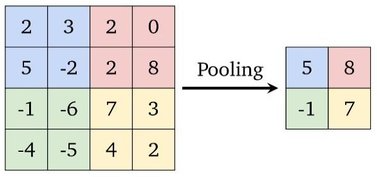
\includegraphics[width=0.4\linewidth]{images/pool_max.png}}
\hfill
\subfigure[Average Pooling]{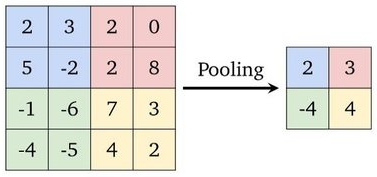
\includegraphics[width=0.4\linewidth]{images/pool_avg.png}}    
\caption{Example of Max Pooling and Average Pooling operations performed over a feature map of $4 \times 4$ with $pool\_size=2 \times 2$, $stride=2$, and no padding. Adapted from \citep{guissousallaeddine2019}.}
\label{fig:poolings}
\end{figure*}

The pooling layer has three input parameters: the filter size (also called pool size), the stride, and whether to apply padding to the input image. Commonly, the filter size is $2 \times 2$, the stride is 2, and no padding is applied. Using this configuration, the feature map is reduced by half at each dimension, and 75\% of the original activations are discarded. The number of channels of the feature map (depth) remains unchanged.

There is a special kind of pooling known as \textbf{global pooling}, introduced by \cite{lin2013network}. In addition to the traditional method, the global version extends the pooling across the entire feature map. Therefore, if a given feature map has $H \times W \times C$ dimensions, it will be reduced to $1 \times 1 \times C$. Again, the most common functions used in global pooling are maximum and average. As stated by \cite{zhou2016learning}, such difference makes global pooling layers perform better in practice than the conventional approach. Moreover, it can substitute the flattened layers in the transition between convolutional layers and the fully connected network responsible for outputting a prediction.

Since pooling computes a fixed function of the input, no learning parameters are required by the pooling layers in Convolutional Networks. This is valid for all pooling approaches described above (max, average, and global pooling).

\paragraph{Batch Normalization Layers}

The task of training deep neural networks can be challenging due to many factors. For example, we can cite the random weights initialization, the optimization algorithm, and the chosen hyperparameters configuration. Furthermore, during the learning phase, each parameter is updated by the gradient under the assumption that the other layers do not change \citep{goodfellow2016deep}. However, in practice, all layers are updated simultaneously.

Another significant factor is related to the expectations around layer distributions. During training, the distribution of each layer's input changes as previous layers' parameters also change. This is referred to as Internal Covariate Shift \citep{ioffe2015batch}. It may cause unintended effects in the training of deep networks since small changes in shallower layers will be amplified during a forward pass to deeper hidden layers.

Batch Normalization is a regularization technique proposed by \cite{ioffe2015batch} to mitigate the effect of Internal Covariate Shift. It normalizes the inputs of hidden layers using the first (mean) and second (variance) statistical moments of the current batch. This normalization step is usually applied before the activation function but can also be employed after the non-linear function. The batch normalization makes the training of deep neural networks faster, more stable, and less likely to overfit. Also, the batch normalization may substitute the use of Dropout as a regularization technique.

Given a mini-batch $B$ of size $m$, the mean and variance of $B$ are denoted by Equations \ref{eq:bn_mean} and \ref{eq:bn_stddev}, respectively:

\begin{equation}
\label{eq:bn_mean}
\mu_B = \frac{1}{m} \sum_{i}^{m} x_i
\end{equation}

\begin{equation}
\label{eq:bn_stddev}
\sigma_B^2 = \frac{1}{m} \sum_{i=1}^{m} (x_i - \mu_B)^{2}
\end{equation}

Then, the input $x_i$ is normalized by \autoref{eq:bn_norm}:

\begin{equation}
\label{eq:bn_norm}
\hat{x}_i = \frac{x_i - \mu_B}{\sqrt{\sigma_B^{2} + \epsilon}}
\end{equation}

\noindent
where $x_i$ can be either the input or output of the activation function from the current layer, and $\epsilon$ is a arbitrarily small constant added for numerical stability. The final output $y_i$ of the current layers is given by \autoref{eq:bn_output}:

\begin{equation}
\label{eq:bn_output}
y_i = \gamma\hat{x}_i + \beta
\end{equation}

\noindent
where $\gamma$ and $\beta$ are new learnable parameters introduced by batch normalization. 

One important aspect to notice is the fact that the batch normalization operation can be automatically avoided by the network. I.e., if the network during training realizes that the input $x_i$ does not need to be normalized, it can set $\gamma=1$ and $\beta=0$, so the input $x_i$ remains unchanged.

During the training phase, the normalization steps are computed based on mini-batches to ensure reliable and efficient training. On the other hand, during inference, the network is generally asked to perform prediction given a single sample. For this reason, the normalization step is performed with the population statistics estimated. The population mean and variance are estimated during training and are defined by Equations \ref{eq:bn_pop_mean} and \ref{eq:bn_pop_var}, respectively: 

\begin{equation}
\label{eq:bn_pop_mean}
E[x] = E_B[\mu_B]
\end{equation}

\begin{equation}
\label{eq:bn_pop_var}
Var[x] = \frac{m}{m-1} E_B[\sigma_B^{2}]
\end{equation}

Therefore, during inference, the input $x$ will be normalized by \autoref{eq:bn_inf_xi}:

\begin{equation}
\label{eq:bn_inf_xi}
\hat{x} = \frac{x - E[x]}{\sqrt{Var[x] + \epsilon}}
\end{equation}

And the output $y$ will be given by \autoref{eq:bn_inf_yi}:

\begin{equation}
\label{eq:bn_inf_yi}
y = \frac{\gamma}{\sqrt{Var[x] + \epsilon}} \cdot \hat{x} + \left( \beta - \frac{\gamma E[x]}{\sqrt{Var[x] + e}} \right)
\end{equation}

The implementation of batch normalization for \aclp{cnn} is slightly different in comparison to the fully connected networks. Since the output of \acs{cnn} layers can have multiple channels, batch normalization is carried out for each of these channels. In other words, each channel will have a single mean and standard deviation as well as scale ($\gamma$) and shift ($\beta$) parameters. Again, they are scalar values learned during the optimization process. Similarly, the batch normalization procedure can be applied before or after the non-linear activation function of the correspondent convolutional layer.

Besides reducing the internal covariate shift, batch normalization also has some other valuable advantages. Firstly, it can speed up training since we can use higher learning rates without vanishing or exploding the gradients. Secondly, it can make the network more robust to different initialization schemes and learning rates. Finally, since batch normalization is a regularization technique, it helps the network improve in terms of generalization and diminish overfitting. As pointed out earlier, batch normalization can replace other regularization methods like Dropout.

Although the effect of batch normalization is evident, the explanation of why it works is still an open question. For example, some authors have suggested that the batch normalization does not reduce the internal covariance shift but actually smooths the objective function \citep{santurkar2018does}. Notwithstanding, batch normalization leads to harsh gradient explosion in deep networks at initialization, but such effect is mitigated by skip connections like the ones in residual networks \citep{yang2019mean}. Other authors suggest that the training of neural networks is faster with batch normalization due to the length-direction decoupling achieved by this technique \citep{kohler2019exponential}.

\subsubsection{Autoencoders}

Autoencoders represent a specific type of neural network capable of discovering structure within data to create a compressed representation of the input. They are considered an unsupervised (or self-supervised) learning technique to leverage the neural networks for representation learning. In the last years, Autoencoders have been successfully applied to many different tasks like: dimensionality reduction \citep{petscharnig2017dimensionality, wang2015dimensionality}, information retrieval tasks \citep{pfeiffer2018neural}, anomaly detection \citep{sakurada2014anomaly}, and image segmentation \citep{baur2018deep, karimpouli2019segmentation}.

The architecture of Autoencoders (\autoref{fig:autoencoder}) is usually composed of two parts:

\begin{figure}[h]
\centering
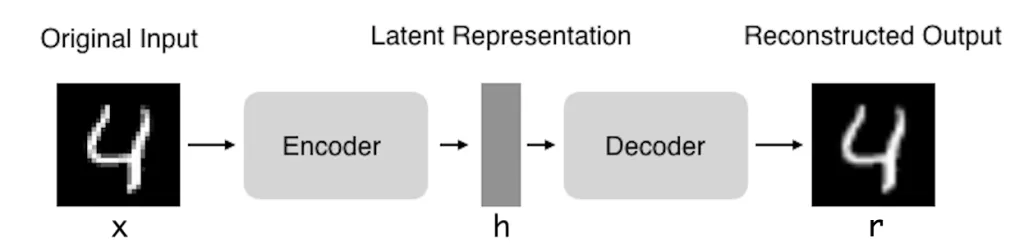
\includegraphics[width=\linewidth]{images/autoencoder.png}
\caption{Architecture of an Autoencoder. Source: \citep{autoencoder_architecture}}
\label{fig:autoencoder}
\end{figure}

\begin{enumerate}
\item \textbf{Encoder}: responsible to learn an useful representation of the input, also called \textbf{embeddings} or \textbf{latent representation} or even \textbf{code}. It can be formulated as an encoder function $h = f(x)$, where $x$ is the input and $h$ corresponds to the codification of the input in the latent space ($h: \mathbb{R}^D \rightarrow \mathbb{R}^K$, where $D$ and $K$ represent the dimensionality of the input and the latent space, respectively).

\item \textbf{Decoder}: maps the learned latent representation $h$ back to the original input space ($\mathbb{R}^K \rightarrow \mathbb{R}^D$). It can be described as a reconstruction function $r = g(h)$, where $r$ is the reconstructed input.
\end{enumerate}

Since the exact copy of the input, $g(f(x)) = x$, is not especially useful, Autoencoders are intentionally designed to be unable to learn a perfect copy. Usually, Autoencoders are regularized in ways that allow them to learn an approximation of the identity function. By forcing the model to prioritize which input elements are relevant for reconstruction,  it often learns valuable properties of the data.

One typical Autoencoder architecture restricts the embedding dimensions ($h$) to be smaller than the input $x$. Such Autoencoder is called \textbf{undercomplete}. By constraining $h$, the Autoencoder is forced to learn an undercomplete representation and must prioritize the most salient features of the input data during training. Moreover, the reconstructed input $r$ will not be a perfect copy of the input, and the undercomplete Autoencoders can be considered lossy compressors.

The learning process of Autoencoders involves the minimization of a loss function like \autoref{eq:loss-basic}:

\begin{equation}
\label{eq:loss-basic}
L(x, g(f(x)))
\end{equation}

\noindent
where $L$ is a loss function that computes the similarity between the reconstructed input $g(f(x))$ and the original input $x$. For instance, $L$ can be the \acf{mse} or \acf{mae}

If the decoder is linear and $L$ is the \acs{mse}, the undercomplete Autoencoder will generate a subspace similar to PCA, described later in Section \ref{sec:pca} \citep{lecun2015deep}. On the other hand, Autoencoders with both non-linear encoder and decoder can learn a more powerful representation than PCA. However, if the encoder and decoder are too powerful, the Autoencoder can learn the identity function without extracting useful information about the data distribution. For instance, each training sample $x^{(i)}$ can be expressed as the code $i$, and the decoder can learn to map these integer indices back to the specific training examples. Nonetheless, it is rare to occur in practice \citep{lecun2015deep}.

Although the training of Autoencoders is similar to regular Neural Networks, some hyperparameters require special attention, like:

\begin{itemize}
\item \textbf{Embedding size}: the size of the latent representation represents a trade-off between compression and accurate reconstruction. Smaller size results in more compression, but the Autoencoder may be forced to drop relevant features for reconstruction. On the other hand, the higher the embedding size, the more likely is the Autoencoder to simply memorize or overfit the training data. Usually, this effect can be diminished by adding a term to the loss function that discourages memorization/overfitting (for instance, a regularizer).

\item \textbf{Number of Layers}: Vanilla Autoencoders are trained with a single hidden layer. However, training multilayer Autoencoders offers many advantages. First, depth can exponentially reduce the computation cost associated with representing some function. Furthermore, depth can also decrease the amount of training data needed to train a useful Autoencoder \citep{lecun2015deep}. Finally, experiments have shown that deep Autoencoders yield much better compression than equivalent shallow or linear Autoencoders \citep{hinton2006reducing}.

\item \textbf{Number of nodes per layer}: usually, Autoencoders have symmetric architecture. The number of nodes per layer in the encoder is the same as the decoder part but inverse. In the case of undercomplete Autoencoders, described earlier, the number of neurons per layer decreases at each layer and increases back in the decoder. In fact, symmetric architecture is not a mandatory rule but is commonly adopted in practice.

\item \textbf{Loss Function}: as discussed before, generally the \acs{mse} and \acs{mae} are used to measure the differences between the original input and the consequent reconstruction. Similarly, for the cases where the input is in the range [0-1], binary cross-entropy may also be used. However, other types of Autoencoders can apply different loss functions. For example, the Sparse Autoencoders adds a sparsity constraint (e.g., L1 regularization) as a penalty term such that only a fraction of the nodes will become active (i.e., nonzero values).
\end{itemize}

As pointed by \cite{lecun2015deep}, the lower-dimensional representations of Autoencoders have some benefits, like (i) it can improve the performance of tasks such as classification; (ii) fewer parameters require less memory and runtime; and (iii) the hints provided by the lower-dimensional space aid generalization.

\subsubsection{Multitask Learning}

\acf{mtl} is a recent machine learning technique in which multiple tasks are solved simultaneously, exploring common aspects and differences between them. This technique is inspired by the human learning process, where the knowledge obtained in previous problems is applied to learn the pattern of a new problem \citep{zhang2017survey}. Through \acs{mtl}, the network can use relevant information in related tasks to improve generalization in all tasks. Besides, this technique is best suited when there are limited training samples in multiple related tasks.

From the \acl{ml} point of view, \acl{mtl} can be seen as a form of inductive transfer. The goal of inductive transfer is to take advantage of additional information sources to increase the performance of the current task learning. It helps a model by introducing an inductive bias. Therefore, a model can prefer some hypotheses over others. A typical example of inductive bias is L1 regularization, which leads a model to prefer sparse solutions. In the context of \acs{mtl}, the inductive bias is supplied by the auxiliary tasks. In this case, the model will give preference to the hypothesis that explains more than one task. According to \cite{Caruana1997}, the inductive transfer can decrease the time of the learning process and increase the generalization and intelligibility of the model. 

Historically, \acs{mtl} methods were classified into hard or soft parameter sharing techniques \citep{vandenhende2021multi}. In the hard parameter sharing, initially proposed by \cite{Caruana1997}, the network parameters are divided into shared and task-specific parameters. Typically, \acs{mtl} models using hard parameter sharing contain a shared encoder with task-specific branches \citep{kendall2018multi, chen2018gradnorm, sener2018multi}. As proved by \cite{baxter1997bayesian}, the risk of overfitting in hard parameter sharing is order $N$ smaller than overfitting the task-specific branches, where $N$ is the number of tasks. Intuitively, since it is harder for a model to find a shared representation for all tasks, the less likely is the chance of overfitting. On the other hand, in soft parameter sharing, the parameters of each task are handled by a feature sharing mechanism \citep{ruder2019latent, gao2019nddr, liu2019end}. In this case, each task has a specific model, and the parameters of each model are regularized to be similar. \autoref{fig:mtl_sharing} visually explains the differences between hard and soft parameters sharing.

\begin{figure*}[ht]
\centering
\subfigure[Hard Parameter Sharing]{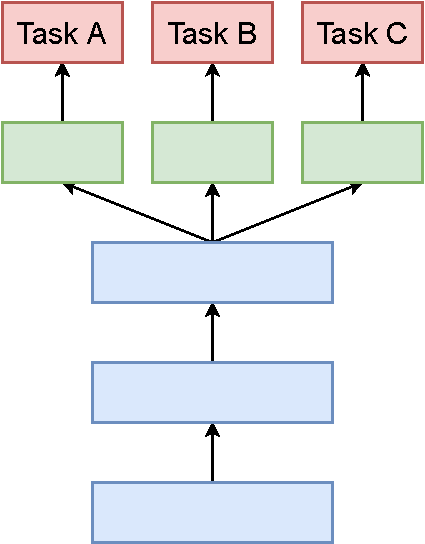
\includegraphics[height=0.35\linewidth]{images/mtl_hard.pdf}}
\hfill
\subfigure[Soft Parameter Sharing]{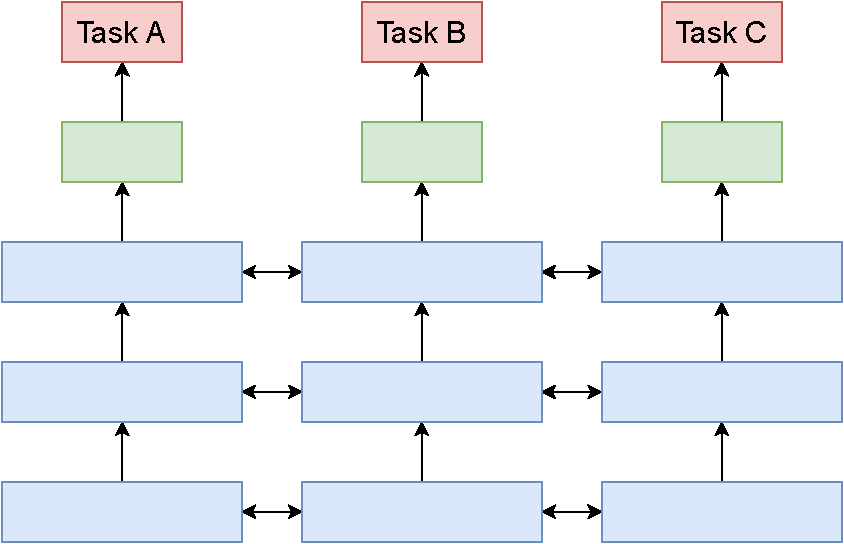
\includegraphics[height=0.35\linewidth]{images/mtl_soft.pdf}}    
\caption{Types of parameter sharing in \acl{mtl}. Source: own elaboration.}
\label{fig:mtl_sharing}
\end{figure*}

Compared to the case where each task of a multitask problem is solved individually by a specific network, the multitask networks present several advantages. First, the amount of parameters and memory used by the model is considerably reduced due to the inherent layer sharing. Secondly, the inference speed increases since such networks avoid the recomputation of features in the shared layers. Finally, such networks can improve performance if the related tasks share complementary information or act as a regularizer for one another \citep{vandenhende2021multi}. 

% In the context of the \icao standard, the MTL can be used to solve all requirements in parallel, reducing the processing time and increasing the success rates.

% \textbf{Multitask Optimization}. The optimization in MTL is still a significant challenge mainly because multiple learning procedures are being accomplished simultaneously. Therefore, one or more tasks can dominate the network weights or influence the gradients in opposite directions. To handle these problems, many approaches have been proposed in the literature over the years and will be discussed below.

% We can formulate the optimization of multitask problems without loss of generality as a function of task-specific weights $w_i$ and task-specific loss functions $\mathcal{L}$:

% \begin{equation}
% \label{eq:multitask-loss}
% \mathcal{L}_{MTL} = \sum_i {w_i \cdot \mathcal{L}_i}
% \end{equation}

% By using stochastic gradient descent to minimize the Eq. \ref{eq:multitask-loss}, the networks weights of a shared layer $W_sh$ are updated by the following rule:

% \begin{equation}
% \label{eq:multitask-sgd}
% W_{sh} = W_{sh} - \gamma \sum_i {w_i \frac{\partial \mathcal{L}_i}{\partial W_{sh}}}
% \end{equation}

\subsubsection{Network Explainability and Visualization}

For some time, Deep Learning methods were considered black boxes since the interpretation of its outputs was hard to explain. To overcome this problem, some methods to visualize and explain predictions of Neural Networks have been proposed in the specialized literature. Some of the most well-known methods includes GradCam \citep{gradcam}, LIME \citep{lime}, DeepLIFT \citep{deeplift_old, deeplift_new}, and \acs{shap} \citep{shap2018}. In this section, we focus on detailing \acs{shap} since it is used to analyze the predictions of the proposed method. Furthermore, we cite other variations of \acs{shap} and highlight its advantages.

\paragraph{SHAP}

The \acf{shap} is a method to explain the output of any machine learning model using a solid theoretical foundation of game theory. The classic Shapley values \citep{shapley1953value} from game theory and their related extensions are combined to optimal credit allocation with local explanations. Nowadays, the method is considered the state-of-art method for \acs{ml} explainability.

The basic idea of \acs{shap} comes from the game theory. In summary, the Shapley values try to quantify the contribution that each player brings to a game. In the context of \acl{ml}, the ``game'' is considered as the outcome of the model, while the ``players'' are represented by one or more features included in the model. In the case of images, specifically, pixels can be grouped (superpixels) to explain predictions distributed among them. Therefore, the goal of SHAP is to measure the contribution of each feature concerning the model's prediction.

Given the original prediction model $f$ to be explained and the explanation model $g$, the Shapley value explanation is represented as an additive feature attribution method (\autoref{eq:shap_add}), which is a linear function of binary values:

\begin{equation}
\label{eq:shap_add}
g(z')=\phi_0+\sum_{j=1}^M\phi_jz_j'
\end{equation}

\noindent
where $z' \in \{0,1\}^M$ is the coalition (subset) vector, $M$ is the number of simplified input features (coalition size) and $\phi \in \mathbb{R}$ is the feature attribution for a feature $j$ (Shapley values). Many methods has explanation models that matches the \autoref{eq:shap_add}, including \acs{lime} \citep{lime} and \textit{DeepLIFT} \citep{deeplift_old, deeplift_new}.

To compute the contribution of each feature ($\phi_i$), the \acs{shap} method requires retraining the model on all subset of features $S \subseteq F$, being $F$ the full set of features. A corresponding importance value will be assigned to each feature to represent the effect on the model prediction when such feature is included. To compute this effect, a model is trained with the presence of that feature ($f_{S \cup \{i\}}$), and another model is trained without that feature ($f_S$). Then, the predictions of the two models are compared for the current input $f_{S \cup \{i\}}(x_{S \cup \{i\}}) - f_S(x_S)$. In this case, $x_S$ denotes the values of the input features in the set $S$. The preceding differences are computed for all possible subsets since the effect of withholding a feature also depends of other features in the model. The Shapley values are the weighted average of all possible differences (\autoref{eq:shapley-values}):

\begin{equation}
\label{eq:shapley-values}
\phi_i = \sum_{S \subseteq F \setminus \{i\}} \frac{\left|S\right|!(\left|F\right| - \left|S\right| - 1)!}{\left|F\right|!}\left[f_{S \cup \{i\}}\right (x_{S \cup \{i\}}) - f_S(x_S)]
\end{equation}

Since a model is trained for every subset of $S$, the exact computation of Shapley values is computationally expensive. For $\left|F\right|$ features, there is a total of $2^{\left|F\right|}$ subsets of S. However, in the paper of \acs{shap} \citep{shap2018}, the authors propose a model-agnostic approach to approximate them, called Kernel SHAP, and other four model-type-specific approximation methods: Linear SHAP, Low-Order SHAP, Max SHAP, and Deep SHAP. The Deep SHAP is a specific version of \acs{shap} especially designed for Deep Networks. The method is based on DeepLift \citep{deeplift_old, deeplift_new}, which approximates SHAP values by considering the input features as independent of each other and the deep model as linear. In Deep SHAP, the SHAP values of the whole network are a combination of SHAP values computed for smaller components of the network. It generates an effective linearization from the SHAP values computed for each component. Please, refer to the original paper for further explanations on the other methods.

The SHAP method has the four properties of classical Shapley values:

\begin{enumerate}
\item \textbf{Efficiency:} the sum of the Shapley values for all players is equal to the value of the total coalition. 
\item \textbf{Symmetry}: all players have a fair chance to join the game.
\item \textbf{Dummy}: if a player $i$ has no contribution to a coalition $S$ (i.e., for each $S$, $f_{S \cup \{i\}} = f_S$), then its contributions is zero ($\phi_i = 0$).
\item \textbf{Additivity}: for any pair of games $a$ and $b$, $\phi(a + b) = \phi(a) + \phi(b)$. Such property enables simple arithmetic summations.
\end{enumerate}

Some of the main advantages of \acs{shap} are discussed next. First, it is model agnostic, i.e., \acs{shap} makes no prior assumption of the model and can work with any \acs{ml} algorithm. Secondly, the method ensures consistency. It means that even if features are removed from data, the others keep contributing with the same importance (Shapley values). Lastly, \acs{shap} can explain not only how each feature contributes regarding each sample (\textit{local interpretability}), but also at a global level (\textit{global interpretability}) by aggregating the local results.

\subsection{Dimensionality Reduction}

There are many applications for algorithms of dimensionality reduction. Usually, these methods are used when the cardinality of features is significantly larger than the number of samples (also called the ``\textit{curse of dimensionality}''). However, they may also be applied to project data into a lower-dimensional space (usually 2D/3D), aiming to simplify visualization and the search for patterns in data. In this subsection, two methods of dimensionality reductions used in this work are described.

\subsubsection{Principal Component Analysis}
\label{sec:pca}

The \acf{pca} \citep{pca} is an unsupervised \acl{ml} algorithm for dimensionality reduction with minimal information loss. In PCA, the information is based on the data variance. The idea is that features with high variance contain more information because their data are more distributed than features with low variance. Accordingly, the PCA projects the data into a subspace where the axis with the highest variances, also called \textit{principal components}, are preserved. More details of PCA are described below.

The main step of PCA is to compute the \textbf{eigenvectors} (principal components) of the input data. The eigenvectors explain the variance of data along the new axes and determine the direction in the new feature space. In PCA, they are organized into a projection matrix, and each eigenvector is associated with an \textbf{eigenvalue}. The eigenvalue can be interpreted as the magnitude of the corresponding eigenvector. If the eigenvalues have a similar magnitude, it can be considered a valuable indicator that the original data is already in a suitable subspace. Otherwise, if the magnitude of some eigenvalues is much higher than others, the corresponding eigenvectors may be chosen since they contain more information about our data distribution. Likewise, the eigenvalues near zero are less informative and may be discarded in the construction of the new subspace. 

The classical approach of PCA \citep{pca} computes the covariance matrix, where each element represents the covariance between two features, computed by \autoref{eq:covariance}:

\begin{equation}
\label{eq:covariance}
\sigma_{jk} = \frac{1}{n-1}\sum_{i=1}^{n}(x_{ij} - \bar{x_j})(x_{ik} - \bar{x}_k)
\end{equation}

\noindent
which can be rewritten in matrix form as \autoref{eq:covariance2}:

\begin{equation}
\label{eq:covariance2}
S = \frac{1}{n-1}((x - \bar{x})^T(x - \bar{x}))
\end{equation}

\noindent
where $\bar{x}$ is a D-dimensional vector in which each value corresponds to the average of each feature, and $n$ is the number of features per sample. Also, $x$ is the data matrix, where a row represents each sample, and the features are columns. In practice, if we have a dataset with four features, for instance, the covariance matrix will have the following structure:

$$
\begin{bmatrix}var(1) & cov(1,2) & cov(1,3) & cov(1,4) 
\\ cov(1,2) & var(2) & cov(2,3) & cov(2,4)
\\ cov(1,3) & cov(2,3) & var(3) & cov(3,4)
\\ cov(1,4) & cov(2,4) & cov(3,4) & var(4)
\end{bmatrix}
$$

\noindent
where the main diagonal corresponds to the variance of each dimension, and the remaining elements are the covariance between each dimension pair. An interesting property of the covariance matrix is that the sum of the main diagonal is always equal to the sum of eigenvalues.

The eigenvectors and eigenvalues of PCA can also be computed using the correlation matrix. Although the resulting matrices are different, they will result in the same eigenvectors and eigenvalues since the correlation matrix is given by the standardization of the covariance matrix (\autoref{eq:correlation}):

\begin{equation}
\label{eq:correlation}
corr(x,y) = \frac{cov(x,y)}{\sigma_x \sigma_y}
\end{equation}

Given the projection matrix $W$ computed by PCA, we can project our original data $x$ into the new subspace $S$ by applying the \autoref{eq:pca_transform}:

\begin{equation}
\label{eq:pca_transform}
S = (x-\bar{x}) \times W
\end{equation}

Note that we can rollback to our original space $x$ by application of \autoref{eq:pca_inverse}:

\begin{equation}
\label{eq:pca_inverse}
x = (S \times W^{-1}) + \bar{x}
\end{equation}

Finally, the \acf{lda} \citep{izenman2013linear} is a similar dimensionality reduction technique. In contrast to \acs{pca}, the \acs{lda} is a supervised method that maximizes the component axes for class-separation. Although it looks like \acs{lda} performs better than \acs{pca} in reducing dimensionality for classification problems, this is not always true. Performance comparison in terms of accuracy for image recognition problems has shown that \acs{pca} has performed better than \acs{lda} if the number of samples per class is relatively low \citep{martinez2001pca}.

\subsubsection{t-SNE}

The \acf{tsne}, developed by \cite{tsne}, is a non-linear method of dimensionality reduction that is particularly well suited for visualization of high-dimensional datasets. It is based on Stochastic Neighbor Embedding \citep{sne}, but the main difference is the utilization of the \textit{t}-Student distribution to represent the data in low dimensions.

The \acs{tsne} algorithm has two main stages. First, the symmetric probability of points in the original high-dimensional space is computed. Higher probabilities are assigned to similar points, while dissimilar points are assigned a lower probability. Such probabilities are computed using a \textit{t}-Student kernel with a given degree of freedom. Secondly, a similar probability distribution is defined over the points mapped into the low-dimensional space. The Kullback-Leibler divergence (also called relative entropy) between these two distributions is minimized through a gradient descent technique. A simplified version of \acs{tsne} is shown in Algorithm \ref{alg:tsne} and the details are explained below.

\begin{algorithm}[t]
\caption{Simple version of t-Distributed Stochastic Neighbor Embedding}
\label{alg:tsne}
\begin{algorithmic}
    \State \textbf{Data:} data set $X = \{x_1, x_2, ..., x_n\}$,
    \State cost function parameter: perplexity $\rho$,
    \State optimization parameters: number of iteration $T$, learning rate $\eta$, momentum $\alpha(t)$.
    \State \textbf{Result:} low-dimensional data representation $\gamma^{(T)} = \{y_1, y_2, ..., y_n\}$.
    \Begin 
        \State compute pairwise affinities $p_{j|i}$ with perplexity $\rho$ (using \autoref{eq:tsne_pij})
        \State set $p_{ij} = \frac{p_{j|i} + p_{i|j}}{2n}$
        \State sample initial solution $\gamma^{(0)} = \{y_1, y_2, ..., y_n\}$ from $\mathcal{N}(0, 10^{-4}I)$
        \For{i=1}{T}
        \Begin
            \State compute low-dimensional affinities $q_{ij}$ (using \autoref{eq:tsne_qij})
            \State compute gradient $\frac{\partial C}{\partial \gamma}$ (using \autoref{eq:tsne_grad})
            \State set $\gamma^{(t)} = \gamma^{(t-1)} + \eta \frac{\partial C}{\partial \gamma} + \alpha(t)(\gamma^{(t-1)} - \gamma^{(t-2)})$
        \End
    \End
\end{algorithmic}
\end{algorithm}

Given an object $i$, and each potential neighbor $j$ in the high-dimensional space, the joint probability $p_{ij}$ that computes the pairwise similarity between $i$ and $j$ is defined as in \autoref{eq:tsne_pij}:

\begin{equation}
\label{eq:tsne_pij}
p_{ij} = \frac{exp(-d_{ij}^2)}{\sum_{k \neq i}exp(-d_{ik}^2)}
\end{equation}

In the original SNE, a conditional probability $p_{i|j}$ is used instead. Also, the t-SNE employs the scaled Euclidean Distance as the dissimilarity metric $d_{ij}^2$ between two high-dimensional points $x_i$ and $x_j$ (\autoref{eq:tsne_dij}). However, other distance metrics can be used when appropriate. One important detail to notice is the fact that he pairwise similarity $p_{ij}$ is not robust to outliers since $\left\| x_i - x_j\right\|^2$ will be large. In theses cases, the values of $p_{ij}$ will be extremely small and the location of its low-dimensional map point will have very little effect over the cost function. In practice, such problem is prevented by computing $p_{ij} = \frac{p_{j|i} + p_{i|j}}{2n}$ instead. This ensures that $\sum_j p_{ij} > \frac{1}{2n}$ for all datapoints $x_i$. As a result, each datapoint $x_i$ has a significant higher contribution to the cost function.

\begin{equation}
\label{eq:tsne_dij}
d_{ij}^2 = \frac{\left\| x_i - x_j \right\|^2}{2\sigma_i^2}
\end{equation}

\noindent
where $\sigma_i$ can be either defined by experimentation or via a binary search that makes the entropy of the distribution over neighbors equal to $log\ \rho$. In this case, $\rho$ is an input parameter of the cost function called ``perplexity.'' The perplexity may be interpreted as a measure of the effective number of neighbors and is defined by \autoref{eq:tsne_perp}:

\begin{equation}
\label{eq:tsne_perp}
\rho(P_i) = 2^{H(P_i)}
\end{equation}

\noindent
where $H(P_i)$ is the Shannon entropy of probability $P_i$ measured in bits by \autoref{eq:tsne_entropy}:

\begin{equation}
\label{eq:tsne_entropy}
H(P_i) = -\sum_j p_{j|i}\ log_2\ p_{j|i}
\end{equation}

In general, the performance of t-SNE is reasonably robust to changes in perplexity, and typical values are between 5 and 50.

The similarity in the low-dimensional space is given by \autoref{eq:tsne_qij}:

\begin{equation}
\label{eq:tsne_qij}
q_{ij} = \frac{exp(-\left\| y_i - y_j \right\|^2)}{\sum_{k \neq i} exp(-\left\| y_i - y_k \right\|^2)}
\end{equation}

\noindent
where $y_i$ and $y_j$ represent the low-dimensional counterparts of the
high-dimensional data points $x_i$ and $x_j$. Usually, for tasks in which the dimensionality of the data is reduced to 2D or 3D, the \textit{t}-Student distribution is applied with one degree of freedom and the \autoref{eq:tsne_qij} can be rewritten as \autoref{eq:tsne_qij_1}:

\begin{equation}
\label{eq:tsne_qij_1}
q_{ij} = \frac{(1 +\left\| y_i - y_j \right\|^2)^{-1}}{\sum_{k \neq l} (1 +\left\| y_k - y_l \right\|^2)^{-1}}
\end{equation}

Finally, the \acs{tsne} tries to minimize a single Kullback-Leible divergence (\autoref{eq:tsne_cost}) between a joint probability distribution $P$ in the high-dimensional space and a joint probability distribution $Q$ in the low-dimensional space:

\begin{equation}
\label{eq:tsne_cost}
C = KL(P||Q) = \sum_i\sum_j p_{ij} log \frac{p_{ij}}{q_{ij}}
\end{equation}

In contrast to the SNE implementation, the \acs{tsne} is symmetric since $p_{ij} = p_{ji}$ and $q_{ij} = q_{ji}$ $\forall i,j$. The main advantage of such symmetry is the simpler gradient expression, being faster to compute. The gradient of the cost function $C$ with respect to the point $y_i$ is given by \autoref{eq:tsne_grad}:

\begin{equation}
\label{eq:tsne_grad}
\frac{\partial C}{\partial y_i} = 4 \sum_j (p_{ij} - q_{ij})(y_i - y_j)
\end{equation}

And the set $\gamma^{(t)} = \{y_1, y_2, ..., y_N\}$ will be updated by a momentum term given by \autoref{eq:tsne_update}:

\begin{equation}
\label{eq:tsne_update}
\gamma^{(t)} = \gamma^{(t-1)} + \eta\frac{\partial C}{\partial \gamma} + \alpha(t)(\gamma^{(t-1)} - \gamma^{(t-2)})
\end{equation}

\noindent
where $\gamma^{(t)}$ indicates the solution at iteration $t$, $\eta$ is the learning rate, and $\alpha(t)$ represents the momentum at iteration $t$. For derivation of \acs{tsne} gradient, please refer to Appendix A of \citep{tsne}. 

In comparison to \acs{pca}, the \acs{tsne} does not conserve the distances or the densities of the original space. Only the neighborhood is preserved, but up to a certain degree. Furthermore, there is no convergence guarantee to the global optimum of the cost function, and the performance of \acs{tsne} is not clearly defined for general dimensionality reduction tasks. 


\subsection{Performance Measures} \label{sec:measures}

There is a variety of performance measures to evaluate algorithms in binary classification problems. In common, most of these metrics takes into account some of/all the four possible results presents in the binary confusion matrix: \acfp{tp}, \acfp{tn}, \acfp{fp}, and \acfp{fn}. In this subsection, we describe the evaluation metrics used in this work. Comments about the advantages and disadvantages of each one are also made when appropriate. 

\subsubsection{Accuracy}

Accuracy is one of the most used metrics to evaluate binary classifiers. In simple terms, it measures how many predictions were correct among all samples in a given dataset. The output of this metric is a score $\in [0, 1]$ which is interpreted as the proportion of correct predictions (i.e., true positives and true negatives) among the total number of samples analyzed. The Accuracy is described by the \autoref{eq:accuracy}:

\begin{equation}
\label{eq:accuracy}
Accuracy = \frac{TP + TN}{TP + TN + FP + FN}
\end{equation}

Although Accuracy is one of the most used metrics to evaluate binary classifiers, it is not well suited for unbalanced datasets. Suppose we have a dataset where 80\% of samples are from the positive class, and the remaining samples are from the negative class. If some classifier outputs only the positive class, the overall Accuracy will be 80\%. Therefore, Accuracy must only be considered a valid metric when the class distributions are considerably uniform.

\subsubsection{Precision \& Recall} \label{precision-recall}

Precision and Recall are two metrics highly adopted in the evaluation of binary classifiers. While Precision measures how much we can trust a model when it predicts the positive class, the Recall measures how accurate a model is regarding the positive class. In other words, the Precision metric answers the question ``\textit{given the positive predictions, how many were correct?}'', while Recall answers ``\textit{given the positive samples, how many predictions were correct?}''. Precision and Recall are also known as \acf{ppv} and Sensitivity, respectively, and they are defined by Equations \ref{eq:precision} and \ref{eq:recall}: 

\begin{equation}
\label{eq:precision}
Precision = \frac{TP}{TP + FP}
\end{equation}

\begin{equation}
\label{eq:recall}
Recall = \frac{TP}{TP + FN}
\end{equation}

Even though the Precision and Recall metrics are considered more robust than Accuracy to evaluate binary classifiers, both metrics present some drawbacks. First, they are purpose-specific. For example, Precision is a better choice when we want to trust the prediction of the positive class. However, if a model is optimized to maximize Precision only, it can bias the classifier to avoid uncertain positive samples, increasing the false negatives. On the other hand, Recall is more pertinent when we need a classifier that may correctly identify the positive samples, although it can generate more false positives. Hence, in case of a problem where Precision and Recall are equally important, the f-measure may be computed to generate a balanced score between these two metrics. The f-measure is better described in the following subsection.

Secondly, by taking a closer looker at the Equations \ref{eq:precision} and \ref{eq:recall}, we can notice that they do not take into account the True Negatives. Therefore, both metrics are more appropriate when the positive class is more important than the negative class. It is the case of detection problems, for example, where identifying the negative class (usually background) is less important than the positive class (object of interest). Nevertheless, for some classification problems, this is not always true. For instance, we can cite the fraud detection problems, where the correct prediction of the True Negatives has a higher priority over the True Positives. For these cases, we can compute the negative predictive value and specificity metrics, which are described later.

\subsubsection{F-measure}

The f-measure, also called f-score or f1-score, is a metric to balance the values of Precision and Recall. The importance of f-measure is better understood by an example. Suppose there is a face detection problem, where two different models are applied in an image with ten faces, named $A$ and $B$. Model A returned five detections, where 3 were real faces (TP), and 2 were incorrect. In this case, model A has 30\% of Recall (3 out of 10 detected faces) and 60\% of Precision (3 out of 5 correct predictions). Otherwise, model B returned two detections, and they are all real faces. In this case, the Recall is 20\% (2 out of 10 detected faces), and the Precision is 100\% (all detections are real faces). Therefore, if Precision and Recall are equally important for this problem, which model is better: model $A$ with 30\% of Recall and 60\% of Precision, or model $B$ with 20\% of Recall and 100\% of Precision? To answer this problem, we can compute the f-measure, described by \autoref{eq:f-measure}: 

\begin{equation}
\label{eq:f-measure}
F1 = 2\frac{Precision \cdot Recall}{Precision + Recall}
\end{equation}

In the example cited above, the f-measure of model $A$ is 40\%, while the model $B$ is 33.3\%. Therefore, the model $A$ can be considered a better model for this case since it has a higher f-measure and consequently a better equilibrium between Precision and Recall.

By definition, the f-measure is considered the harmonic mean between Precision and Recall. It is harmonic because, in contrast to the arithmetic mean, the metric cannot be made arbitrarily large by changing only Precision or Recall to a bigger value (while keeping the other metric unchanged). Therefore, to increase f-measure considerably, both Precision and Recall must be higher at the same time.

\subsubsection{F-Beta}

The F-Beta is a generalization of the F-measure. It adds a $\beta$ term to weight how much Recall is more important than Precision. The F-Beta is defined by \autoref{eq:f-beta}:

\begin{equation}
\label{eq:f-beta}
F_\beta = \frac{(1 + \beta^2) \cdot P \cdot R}{\beta^2 \cdot P + R}
\end{equation}

As can be noticed, when $\beta=1$, we have the original formula of f1-score. Another typical value is $\beta=2$, generating the f2-score. In this case, we are considering that Recall has a higher weight than precision. In other words, achieving a better Recall is more important for the classifier than Precision. It is useful when we want to make sure that the classifier is better at identifying the positive class, even though it might generate more false positives. In the detection example cited before, the detector would try to detect as many real faces as possible but probably returning more false positives (detections that are not real faces).

\subsubsection{Negative Predictive Value \& Specificity}

The metrics specificity and \acf{npv} are equivalent to Recall and Precision, respectively, but for the negative class. In analogy to Precision and Recall, the specificity answers the question ``\textit{given the negative samples, how many predictions were correct?}'', while the \acs{npv} answers ``\textit{given the negative predictions, how many were correct?}''. The metrics are defined by Equations \ref{eq:specificity} and \ref{eq:npv}:

\begin{equation}
\label{eq:specificity}
Specificity = \frac{TN}{TN + FP}
\end{equation}

\begin{equation}
\label{eq:npv}
NPV = \frac{TN}{TN + FN}
\end{equation}

Since both \acs{npv} and specificity are similar to Precision and Recall, they share the same problems of these metrics described in Section \ref{precision-recall}. Hence, \acs{npv} and specificity are purpose-specific (but, for the negative class) and, analogously, do not take into consideration the positive class.

\subsubsection{\acl{mcc}} \label{sec:mcc}

The \acf{mcc}, also known as phi coefficient, is a binary classification metric that takes into account all four categories: true positives, true negatives, false positives, and false negatives. It was introduced by biochemist Brian W. Matthews in 1975 \citep{matthews1975comparison} and is defined by the \autoref{eq:mcc}

\begin{equation}
\label{eq:mcc}
MCC = \frac{TP \times TN - FP \times FN}{\sqrt{(TP + FP)(TP + FN)(TN + FP)(TN + FN)}}
\end{equation}

The \acs{mcc} is considered a balanced metric and can be used even in highly unbalanced datasets. The output of \acs{mcc} is a normalized coefficient between $-1$ and $+1$. A coefficient of $+1$ means a perfect prediction, while $-1$ represents a total disagreement between prediction and ground truth. Also, a coefficient of $0$ represents that the predictions are no better than random guesses. 

Since the \acs{mcc} takes into account the four possible results of binary classification problems, it presents some advantages in comparison to other classification metrics. For example, given a trained classifier with a confusion matrix of TP = 90, \acs{fp} = 5, TN = 1, and FN = 4, in this case the Accuracy is 91\% and the f-measure is 95.24\%. On the other hand, the \acs{mcc} gives a score of 0.14, which means the algorithm is basically predicting the most frequent class and performing similarly to random guessing. As suggested by \cite{chicco2017ten}, the use of \acs{mcc} is highly encouraged to evaluate the performance in the test set of any binary classification problem.

\subsubsection{Equal Error Rate}

The performance of biometric systems is usually measured by metrics as \acf{far}, \acf{frr}, and \acf{eer}. The \acl{far}, also known as \acf{fmr}, is the probability of an incorrect match between a given input pattern to a non-matching template. In other words, it computes the proportion of invalid inputs that are incorrectly accepted. On the other hand, the False Rejection Rate, also known as \acf{fnmr}, represents the likelihood of a system to falsely reject a match between the input pattern and a genuine matching template. Alternatively, it computes the proportion of valid matches that are incorrectly rejected. According to \cite{ross2006handbook}, the \acs{far} and \acs{frr} can be defined by the Equations \ref{eq:far} and \ref{eq:frr}, respectively:

\begin{equation}
\label{eq:far}
FAR(\tau) = \int_{\tau}^{\infty} p(s|impostor)\ ds
\end{equation}

\begin{equation}
\label{eq:frr}
FRR(\tau) = \int_{\tau}^{\infty} p(s|genuine)\ ds
\end{equation}

\noindent
where $p(s|impostor)$ and $p(s|genuine)$ correspond to the probability distributions of a score $s$ under genuine and impostor conditions, appropriately, and $\tau$ is a threshold to define if a given individual is genuine or an impostor.

Finally, the \acs{eer} is designated by the point where the \acs{far} and \acs{frr} curves intercept each other (see \autoref{fig:eer}). Therefore, the \acs{eer} represents the rate at which both acceptance and rejections errors are equal, i.e., $FAR = FRR$ or $p(s|impostor) = p(s|genuine)$. All the mentioned metrics (\acs{far}, \acs{frr}, and \acs{eer}) are inversely proportional to the performance of the biometric system (the lower, the better).

\begin{figure}[hb]
\centering
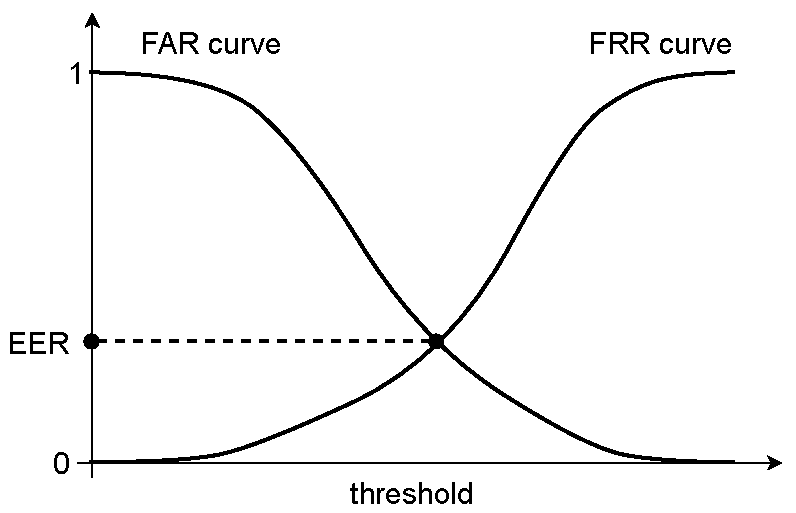
\includegraphics[height=2.1in]{images/EER.pdf}
\caption{The typical curves of the \acs{far} and \acs{frr} error rates, plotted side by side, in relation to the threshold $\tau$ configured for the system. The \acs{eer} is represented by the intersection point of the curves. Source: own elaboration.}
\label{fig:eer}
\end{figure}

Since \acs{far} and \acs{frr} are computed for a given threshold $\tau$, the biometric systems can be calibrated by manually choosing the threshold that best fit the desired needs. However, it represents a trade-off between convenience and security. For example, when security issues are critical (e.g., banking systems), the threshold $\tau$ may be adjusted in a way that the \acs{far} is minimal. However, genuine users may have their access blocked until the system is entirely sure about their profile. On the other side, if $\tau$ is fine-tuned to improve users' convenience, the system can allow access of non-legitimate users.

\subsection{The \icao Standard}

In 1980, the \acf{icao} began a project focused on the standardization of automatic biometric identification of people using machines \citep{icao2003report}. A specific working group was established to determine the most suitable way of ``uniquely encoding a particular physical characteristic of a person into a biometric-identifier that can be machine-verified to confirm the presenter's identity'' \citep{icao2003report}. Initially, three physical attributes were chosen for possible applications: face, fingerprint, and iris. Later, in the ``Berlin resolution'' (2002), the ICAO has chosen the face as the primary globally inter-operable biometric trait for machine-assisted identity confirmation in machine-readable travel documents (MRTDs) \citep{ferrara2012face}. However, the decision also states the possibility of identity confirmation through fingerprint or iris to support the machine-assisted decision.

Following the ICAO guidelines, the \acf{iso}, together with the \acf{iec}, proposed a standard for facial photography to be used in electronic passports. The \icao \citep{iso-iec} standard specifies rules and a record format for encoding, recording, and transmitting facial image information. It also defines a set of environmental conditions, photographic properties, shooting features, and digital image attributes of facial images. For example, a face image may have a uniform background with the absence of shadows in any region of the image to be included in an electronic passport. The complete list of requirements can be seen in Table \ref{tab:icao} and examples of non-compliant images for each requirement are given in Figure \ref{fig:icao}. The \icao standard is also referenced in the ANSI/NIST-ITL 1–2011 standard \citep{nist2011} as one of the standard profiles for face acquisition. In 2019, a new version of the \icao standard was released. The \icaonew provides more detailed information about each requirement evaluation.

\begin{table}[tb]
% \scriptsize
\footnotesize
% \small
\centering
\caption{Description of facial image quality tests performed by \biolab, according to \icao standard.}
\label{tab:icao}
\begin{tabular}{|c|c|}
\hline
\rowcolor[HTML]{9B9B9B} 
\textbf{Req. \#} & \textbf{Test description} \\ \hline
\rowcolor[HTML]{C0C0C0} 
\multicolumn{2}{|c|}{\cellcolor[HTML]{C0C0C0}\textbf{Facial feature extraction tests}} \\ \hline
1 & Eye center location accuracy \\ \hline
2 & Face location accuracy \\ \hline
\rowcolor[HTML]{C0C0C0} 
\multicolumn{2}{|c|}{\cellcolor[HTML]{C0C0C0}\textbf{Geometric tests}} \\ \hline
3 & Eyes distance (min. 90 pixels) \\ \hline
4 & Relative vertical position \\ \hline
5 & Relative horizontal position \\ \hline
6 & Ratio of head width \\ \hline
7 & Ratio of head height \\ \hline
\rowcolor[HTML]{C0C0C0} 
\multicolumn{2}{|c|}{\cellcolor[HTML]{C0C0C0}\textbf{Photographic and pose-specific tests}} \\ \hline
8 & Blurred \\ \hline
9 & Looking away \\ \hline
10 & Ink marked/creased \\ \hline
11 & Unnatural skin tone \\ \hline
12 & Too dark/light \\ \hline
13 & Washed out \\ \hline
14 & Pixelation \\ \hline
15 & Hair across eyes \\ \hline
16 & Eyes closed \\ \hline
17 & Varied Background \\ \hline
18 & Roll/pitch/yaw rotations greater than a predefined thresholds \\ \hline
19 & Flash reflection on skin \\ \hline
20 & Red eyes \\ \hline
21 & Shadows behind head \\ \hline
22 & Shadows across face \\ \hline
23 & Dark tinted lenses \\ \hline
24 & Flash reflection on lenses \\ \hline
25 & Frames too heavy \\ \hline
26 & Frame covering eyes \\ \hline
27 & Hat/cap \\ \hline
28 & Veil over face \\ \hline
29 & Mouth open \\ \hline
30 & Presence of other faces or toys too close to face \\ \hline
\end{tabular}
\end{table}

\begin{figure}[ht]
\centering
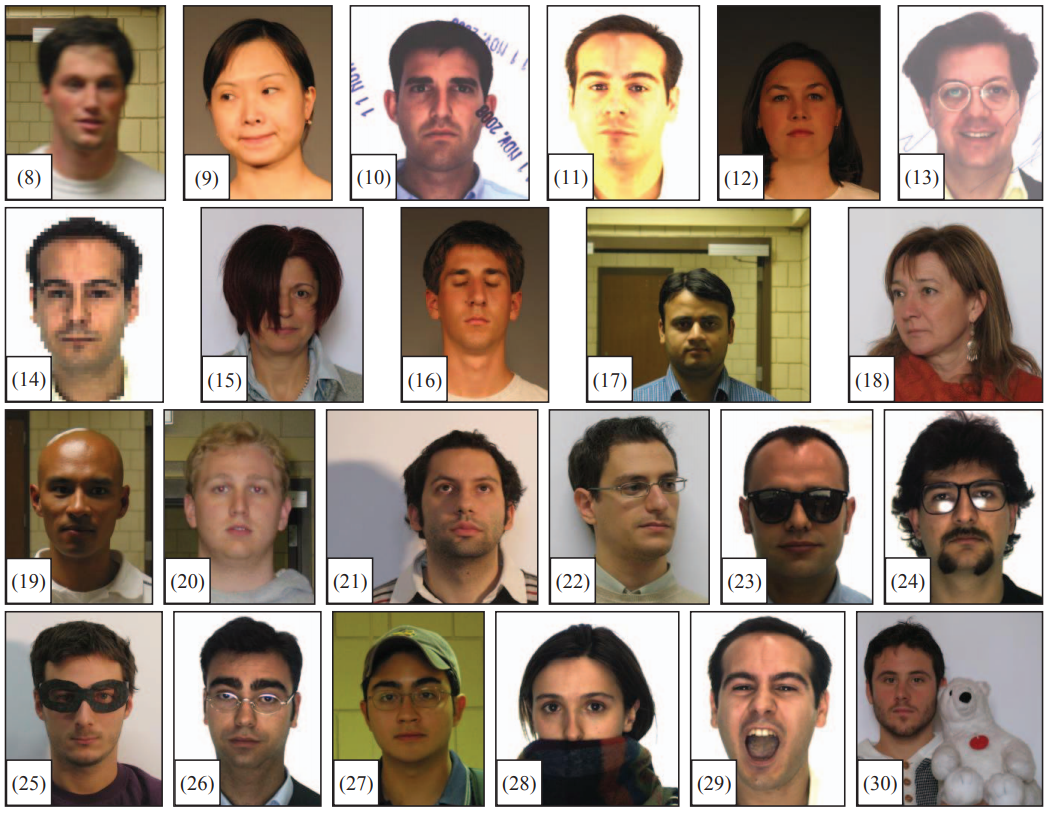
\includegraphics[width=\linewidth]{images/icao.png}
\caption{Examples of non-compliant images for the requirements 8-30 listed in Table \ref{tab:icao}. Source: \cite{maltoni2009biolab}.}
\label{fig:icao}
\end{figure}

\subsection{\fvcongoing} \label{sec:fvcongoing}

The \acf{fvc} is an event organized by four main institutions: \textit{Biometric System Laboratory} (University of Bologna), \textit{Pattern Recognition and Image Processing Laboratory} (Michigan State University), \textit{Biometric Test Center} (San Jose State University), and \textit{Biometric Recognition Group - ATVS} (Universidad Autonoma de Madrid). The main goal of the \acs{fvc} was to benchmark systems that evaluate fingerprint images. Initially, the competitions used to happen biannually (2000, 2002, 2004, and 2006), and such events draw attention from the academic community and the industry related to biometric. Over the years, the \acs{fvc} became a reference in the evaluation of fingerprint systems, allowing research groups, private companies, and even individual developers to compare their methods and follow the state-of-art in fingerprint research.

After 2006, the organizers of \acs{fvc} decided to create the \fvcongoing. It turned the original biannual \acs{fvc} into an ongoing competition, i.e., every participant could register and submit new algorithms in a continuous fashion. Moreover, new competitions regarding fingerprints were added to \fvcongoing, like fingerprint orientation extraction, fingerprint indexing, and minutiae matching.

In 2012, a new benchmark category related to the \icao standard was added to \fvcongoing \citep{ferrara2012face}, called \textit{\acl{ficv}} (\acs{ficv}). The main goal of this benchmark is to evaluate algorithms that assess the compliance of face images to ISO standard. In total, 24 out of 30 requirements are evaluated by the \acs{ficv}: the \citeReq{\eyecenterlocation} and all the photographic and pose-specific tests (8--30) - see \autoref{tab:icao}. Moreover, the \acs{ficv} also evaluates if the image can be converted to a Token Format (see Section 9.2.3 in \citep{iso-iec}) based on the eye positions predicted by a submitted algorithm. In short, an image is considered \textit{tokenizable} (without padding) if:

\begin{itemize}
\item the distance ($E_{Dist}$) between eyes is at least 60 pixels;
\item the rectangular region of size $W \times H$ (with $W=4\cdot E_{Dist}$ and $H=W \cdot 4/3$), determined so that the eyes are horizontally aligned and their center is in position $C_E=(W\cdot1/2,W\cdot3/5)$, is totally enclosed in the original image (see \autoref{fig:icao_token}).
\end{itemize}

\begin{figure}[ht]
    \centering
    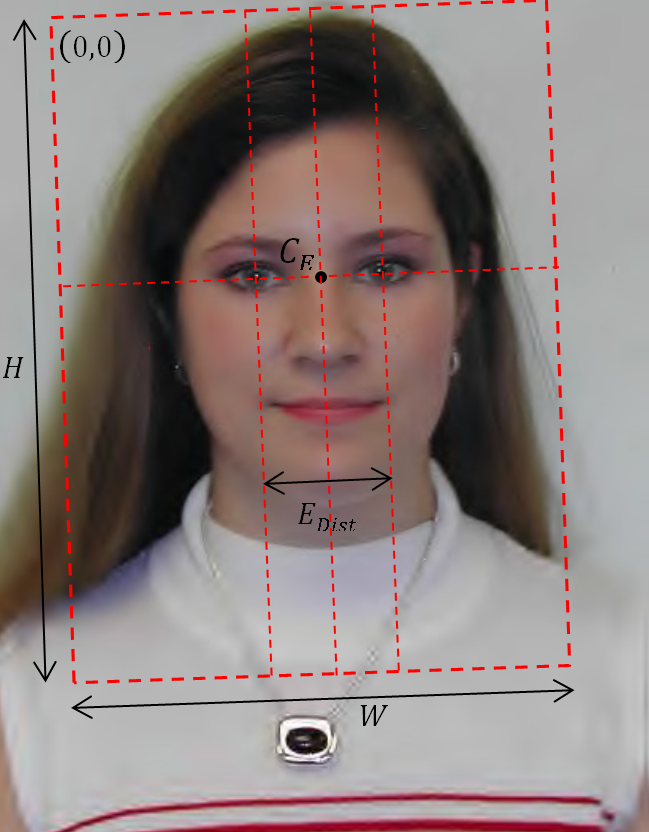
\includegraphics[height=3.0in]{images/icao_tokenizable.png}
    \caption{Geometric characteristics of the token image format. Source: \citep{fvcongoing}.}
    \label{fig:icao_token}
\end{figure}

There are two datasets used to benchmark the algorithms submitted to \acs{ficv} competition: \ficvtest and \ficvofficial. The \ficvtest is a small, but representative dataset (720 images) only used to test the submitted algorithm compliance with the testing protocol (described below). The results computed on this dataset are only visible to the participant and are not considered as official results of the competition. On the other hand, the \ficvofficial contains 4868 images and is private to all participants. Such dataset is detailed in \cite{ferrara2012face}. All the results presented in the literature and in this thesis proposal were computed in the \ficvofficial dataset.

All participants that want to submit an algorithm for evaluation in the \acs{ficv} competition must follow a well-defined protocol. The algorithm must be submitted as a Windows 32 bits (Win32) console application in the format of an executable file. Such executable receives a face image as input and must output the coordinates $(x, y)$ of left-and-right eyes center and a score in the range of $[0, 100]$ to indicate the compliance degree of the input image for each photographic requirement of \autoref{tab:icao}.

Additionally to the submission protocol, the algorithm must still comply with some constraints. For example, the maximum time allowed for the processing of each image is 10 seconds. In case of time violations, the current image evaluation is considered a failure. Also, there is a minimum break of 12 hours between two consecutive submissions by the same participant to the \ficvtest dataset. For the \ficvofficial, this interval is 15 days. However, there are no constraints about memory allocation limit.

Finally, since the requirements \#1 and \#8--30 (see \autoref{tab:icao}) represents different kinds of problems, they are evaluated differently. The \citeReq{\eyecenterlocation} performance is measured by the relative error according to the distances between the expected and the estimated eye positions ($d_{eye}$). This is the same metric introduced by \cite{jesorsky2001robust} and is calculated as follows (\autoref{eq:icao-eyes}):

\begin{equation}
\label{eq:icao-eyes}
d_{eye} = \frac{max(\left\| C_l - \hat{C_l} \right\|, \left\| C_r -\hat{C_r}|\right\|)}{\left\| C_l - C_r \right\|}
\end{equation}

\noindent
where $C_{l/r}$ and $\hat{C_{l/r}}$ represent the ground truth and the positions returned by the algorithm regarding the left and right eyes, respectively. This measure is scale-independent and allows to compare datasets with different image resolutions.

Furthermore, to evaluate the performance of the photographic and pose-specific requirements, the benchmark datasets are divided into 23 different subsets, each related to a specific requirement. Also, each subset contains the same amount of compliant and non-compliant images. Then, for each requirement, the following performance metrics are computed and reported:

\begin{itemize}
\item $EER$: the Equal Error Rate;
\item $FAR_{100}$: the lowest FRR for FAR $\leq$ 1\%;
\item $Zero_{FAR}$: the lowest FRR for FAR=0\%;
\item $Zero_{FRR}$: the lowest FAR for FRR=0\%;
\item $Rejection$: percentage of images where the algorithm did not evaluate the requirement;
\item $Impostor$ and $Genuine$ score distributions;
\item $FAR(\tau) / FRR(\tau)$ curves, where $\tau$ represents the acceptance threshold; and
\item $DET(\tau)$ curve: the Detection Error Tradeoff, which plot the \acl{frr} vs. the \acl{far}.
\end{itemize}

According to \acs{ficv}, the rejections are implicitly included in the computation of metrics in order to discourage the algorithm from rejecting the most uncertain cases and, consequently, improving the performance over the processed images. In these cases, the compliance score is set to 0 in the corresponding requirement of the given image. It follows the best practices of evaluation systems and is also performed in other benchmarks of the \fvcongoing.

In the next chapter, we present a literature analysis related to the current thesis. It focuses on the most relevant published methods for Multitask Learning and the \icao standard, which are the core concepts of the proposed method.

\section{Literature Review} \label{sec:literature}

In this chapter, we start by reviewing deep \acl{mtl} techniques applied in computer vision problems. We focus on different types of deep Multitask architectures and the most famous works published for each category. Additionally, we provide a complete historical review of the methods that addressed the \icao standard, including the methods published in the \fvcongoing website. Finally, we conclude this chapter by discussing relevant findings of the literature review of both topics.

\subsection{Multitask Learning}

A variety of techniques and architectures for \acs{mtl} has been proposed in the literature of Deep Learning. Usually, Deep Multitask Architectures may be divided into encoder-focused and decoded-focused architectures \citep{vandenhende2021multi}. The main characteristic of the encoder-focused architectures \citep{kendall2018multi, chen2018gradnorm, sener2018multi} is the presence of an off-the-shelf backbone network, usually called an encoder. The goal of the encoder is to learn a generic representation that will be shared by a set of independent task-specific heads. Differently, the decoder-focused architectures also exchange information during the decoding stage \citep{xu2018pad, zhang2018joint, vandenhende2020mti}. In the following subsections, we discuss the most relevant Deep \acl{mtl} architectures.

\subsubsection{Encoder-focused Architectures}

The \textbf{Cross-stitch networks} \citep{misra2016cross} combines two given activation maps $x_A$ and $x_B$ - that belongs to tasks $A$ and $B$ respectively -, in a learnable linear way. The transformation can be expressed by learnable weights $\alpha$, as shown in the \autoref{eq:cross-stitch}:

\begin{equation}
\label{eq:cross-stitch}
\begin{bmatrix}
\bar{x}_A\\ 
\bar{x}_B
\end{bmatrix} = 
\begin{bmatrix}
\alpha_{AA} & \alpha_{AB} \\ 
\alpha_{BA} & \alpha_{BB}
\end{bmatrix}
\begin{bmatrix}
x_A \\ 
x_B
\end{bmatrix}
\end{equation}

By using this equation, the Cross-stitch networks can decide the degree to which the features are shared between different tasks. However, to maximize performance, such networks must be pre-trained before stitching them together. Additionally, the size of the cross-stitch network linearly increases with the number of tasks. 

\textbf{Neural Discriminative Dimensionality Reduction CNNs} (NDDR-CNNs) \citep{gao2019nddr} presents a similar architecture with cross-stitch networks. Nonetheless, a dimensionality reduction component is employed instead of the linear combination to merge all single-task networks' activations. However, besides the NDDR-CNNs being susceptible to the same problems, they also require additional design choices (e.g., where to include the NDDR layers). Nevertheless, both networks are limited to local information when the activations from different single-task networks are fused.

The \textbf{Multitask Attention Networks} (MTAN) \citep{liu2019end} are a encoder-focused design that combine the encoder with task-specific attention modules in the backbone network. While the encoder is responsible for computing a general pool of features, the task-specific attention module chooses features from the general pool by applying a soft attention mask. Regular convolutional layers with sigmoids are used to implement the attention mechanism. Compared to cross-stitch networks and NDDR-CNNs, the MTAN model is also limited to local information to produce the attention mask but is less prone to scalability issues.

\subsubsection{Decoder-focused architectures}

One of the first decoder-focused architectures published in the literature was \textbf{PAD-Net} \citep{xu2018pad}. Although the input image is still handled by an off-the-shelf backbone network, the backbone features are further processed by task-specific heads that produce initial predictions for each task. The task-specific heads contain a per-task feature representation of the input image and are recombined by a multi-modal distillation. The main goal of the distillation unit is to extract cross-task information by using a spatial attention mechanism. The output features $F_k^o$ for a given task $k$ are computed by the \autoref{eq:padnet}:

\begin{equation}
\label{eq:padnet}
F_k^o = F_k^i + \sum {\sigma (W_{k,l}F_l^i) \odot F_l^i}
\end{equation}

\noindent where $\sigma (W_{k,l}F_l^i)$ represents the spatial attention mask applied to the initial task features $F_l^i$ from task $l$. However, \autoref{eq:padnet} presumes that task interactions are location independent. Therefore, there must be no relationship between tasks across the entire image.

Similar to PAD-Net, the \textbf{Pattern-Affinitive Propagation Networks} (PAP-Net) \citep{zhang2019pattern}, improved the multi-model distillation. By a statistical observation that pixel affinities contribute to a better alignment with common local structures on the task label space, they proposed to leverage pixel affinities to perform multi-modal distillation. A pixel affinity matrix $M_{T_j}$ is computed by estimating pixel-wise correlations upon the task features coming from each task-specific head. Then, a cross-task information matrix $\hat{M}_{T_j}$ for each task $T_j$ is learned by an adaptive combination of the affinity matrices $M_{T_j}$ for tasks $T_i$ with learnable weights $\alpha_i^{T_j}$, as defined in \autoref{eq:papnet}:

\begin{equation}
\label{eq:papnet}
\hat{M}_{T_j} = \sum_{T_i} {\alpha_i^{T_j} \cdot M_{T_i}}
\end{equation}

The task features of a task $j$ are refined by the cross-task information matrix $M_{T_j}$, which is dissipated across the task features space to spread the pixel correlation for task $T_j$ based on the pixel similarities from the other tasks $T_i$. Unlike the other decoder-focused architectures mentioned, the PAP-Net also models the non-local relationships through pixel similarities computed across the whole image.

The \textbf{Joint Task-Recursive Learning} (JTRL), proposed by \cite{zhang2018joint}, recursively predicts two tasks by increasing higher scales to refine the results of past states gradually. Compared to PAD-Net and PAP-Net, there is also a multi-modal mechanism that combines information from earlier task predictions, which are used to refine the later ones. However, the JTRL model is only able to predict two tasks sequentially and in an intertwined approach. Moreover, the main drawback of the JTRL model is that it is not simple, or even possible, to extend the architecture to more than two tasks because of the intertwined approach to refine predictions.

\subsection{Methods for the \icao standard}

One of the first studies to address the ICAO requirements was proposed by \citet{sang2009face}. It presents methods to evaluate requirements related to illumination conditions and facial pose based on Gabor wavelet features. Furthermore, a method to evaluate the image blur is proposed through the Discrete Cosine Transform (DCT). The authors assess their methods using images from CMU-PIE and FERET datasets. However, only analytical results are presented.

The popularization of methods for \icao standard can be credited to the Biolab group from the University of Bologna. In 2009, they presented the Biolab-ICAO framework \citep{maltoni2009biolab}, a benchmark tool for systems assessing face image compliance to ICAO requirements. In 2012, the benchmark was refined, and the official ground truth face database (4868 images) and testing protocol were presented \citep{ferrara2012face}. Moreover, the authors proposed the BioLabSDK, the first known method published in the literature able to evaluate all the 23 face-and-pose requirements (8--30 in Table \ref{tab:icao}). The BiolabSDK uses different color spaces, face detection, and points that define the face and its elements to generate a score for each requirement. The paper also compares the BioLabSDK against two anonymous SDKs using the Equal Error Rate (EER). The results can be seen in the first three columns of Table \ref{tab:comp}.

% Please add the following required packages to your document preamble:
% \usepackage{graphicx}
% \usepackage[table,xcdraw]{xcolor}
% If you use beamer only pass "xcolor=table" option, i.e. \documentclass[xcolor=table]{beamer}
% \usepackage{lscape}
\begin{landscape}
\begin{table*}[tb]
\centering
\caption{Comparison of methods for the pose and photography requirements (8--30) of the \icao standard. The EER and Rejection Rate are presented for each method and were evaluated by the BioLab-ICAO framework in the FICV competition. The "-" indicates the method does not evaluate that requirement or that results were not informed by the authors.}
\label{tab:comp}
\resizebox{\linewidth}{!}{%
\begin{tabular}{rrrrrrrrrrrrrrrrrrrrrrrrr}
\cline{2-25}
 & \multicolumn{2}{c}{\textbf{SDK1}} & \multicolumn{2}{c}{\textbf{SDK2}} & \multicolumn{2}{c}{\textbf{BioLab}} & \multicolumn{2}{c}{\textbf{BioTest}} & \multicolumn{2}{c}{\textbf{BioPass Face}} & \multicolumn{2}{c}{\textbf{id3}} & \multicolumn{2}{c}{\textbf{ICAO SDK}} & \multicolumn{2}{c}{\textbf{FerraraSeg}} & \multicolumn{2}{c}{\textbf{Borges et al.}} & \multicolumn{2}{c}{\textbf{Andrezza et al.}} & \multicolumn{2}{c}{\textbf{Parente et al.}} & \multicolumn{2}{c}{\textbf{HMAX}} \\ \cline{2-25} 
\textbf{Req. \#} & \multicolumn{1}{c}{EER} & \multicolumn{1}{c|}{{\color[HTML]{9B9B9B} Rej.}} & \multicolumn{1}{c}{EER} & \multicolumn{1}{c|}{{\color[HTML]{9B9B9B} Rej.}} & \multicolumn{1}{c}{EER} & \multicolumn{1}{c|}{{\color[HTML]{9B9B9B} Rej.}} & \multicolumn{1}{c}{EER} & \multicolumn{1}{c|}{{\color[HTML]{9B9B9B} Rej.}} & \multicolumn{1}{c}{EER} & \multicolumn{1}{c|}{{\color[HTML]{9B9B9B} Rej.}} & \multicolumn{1}{c}{EER} & \multicolumn{1}{c|}{{\color[HTML]{9B9B9B} Rej.}} & \multicolumn{1}{c}{EER} & \multicolumn{1}{c|}{{\color[HTML]{9B9B9B} Rej.}} & \multicolumn{1}{c}{EER} & \multicolumn{1}{c|}{{\color[HTML]{9B9B9B} Rej.}} & \multicolumn{1}{c}{EER} & \multicolumn{1}{c|}{{\color[HTML]{9B9B9B} Rej.}} & \multicolumn{1}{c}{EER} & \multicolumn{1}{c|}{{\color[HTML]{9B9B9B} Rej.}} & \multicolumn{1}{c}{EER} & \multicolumn{1}{c|}{{\color[HTML]{9B9B9B} Rej.}} & \multicolumn{1}{c}{EER} & \multicolumn{1}{c}{{\color[HTML]{9B9B9B} Rej.}} \\ \cline{2-25} 
\textbf{8} & 26.00 & {\color[HTML]{9B9B9B} 8.90} & 48.10 & {\color[HTML]{9B9B9B} 0.60} & 5.20 & {\color[HTML]{9B9B9B} 0.00} & 30.50 & {\color[HTML]{9B9B9B} 36.00} & 1.60 & {\color[HTML]{9B9B9B} 3.30} & 1.70 & {\color[HTML]{9B9B9B} 0.20} & 48.80 & {\color[HTML]{9B9B9B} 0.00} & \textbf{-} & {\color[HTML]{9B9B9B} \textbf{-}} & \textbf{-} & {\color[HTML]{9B9B9B} \textbf{-}} & \textbf{-} & {\color[HTML]{9B9B9B} \textbf{-}} & \textbf{-} & {\color[HTML]{9B9B9B} \textbf{-}} & \textbf{-} & {\color[HTML]{9B9B9B} \textbf{-}} \\
\textbf{9} & 27.50 & {\color[HTML]{9B9B9B} 7.10} & \textbf{-} & {\color[HTML]{9B9B9B} \textbf{-}} & 20.60 & {\color[HTML]{9B9B9B} 0.00} & 24.20 & {\color[HTML]{9B9B9B} 3.10} & 13.30 & {\color[HTML]{9B9B9B} 3.30} & 15.30 & {\color[HTML]{9B9B9B} 15.80} & 47.50 & {\color[HTML]{9B9B9B} 2.50} & \textbf{-} & {\color[HTML]{9B9B9B} \textbf{-}} & 16.90 & {\color[HTML]{9B9B9B} 1.20} & \textbf{-} & {\color[HTML]{9B9B9B} \textbf{-}} & \textbf{-} & {\color[HTML]{9B9B9B} \textbf{-}} & 10.00 & {\color[HTML]{9B9B9B} 0.16} \\
\textbf{10} & \textbf{-} & {\color[HTML]{9B9B9B} \textbf{-}} & \textbf{-} & {\color[HTML]{9B9B9B} \textbf{-}} & 3.40 & {\color[HTML]{9B9B9B} 1.20} & 3.60 & {\color[HTML]{9B9B9B} 1.40} & 4.80 & {\color[HTML]{9B9B9B} 0.50} & \textbf{-} & {\color[HTML]{9B9B9B} \textbf{-}} & \textbf{-} & {\color[HTML]{9B9B9B} \textbf{-}} & \textbf{-} & {\color[HTML]{9B9B9B} \textbf{-}} & \textbf{-} & {\color[HTML]{9B9B9B} \textbf{-}} & \textbf{-} & {\color[HTML]{9B9B9B} \textbf{-}} & \textbf{-} & {\color[HTML]{9B9B9B} \textbf{-}} & \textbf{-} & {\color[HTML]{9B9B9B} \textbf{-}} \\
\textbf{11} & 18.70 & {\color[HTML]{9B9B9B} 4.80} & 50.00 & {\color[HTML]{9B9B9B} 0.80} & 4.00 & {\color[HTML]{9B9B9B} 0.20} & 5.10 & {\color[HTML]{9B9B9B} 1.70} & 1.90 & {\color[HTML]{9B9B9B} 0.00} & 2.10 & {\color[HTML]{9B9B9B} 0.20} & 50.00 & {\color[HTML]{9B9B9B} 88.8} & \textbf{-} & {\color[HTML]{9B9B9B} \textbf{-}} & \textbf{-} & {\color[HTML]{9B9B9B} \textbf{-}} & 3.70 & {\color[HTML]{9B9B9B} 0.00} & \textbf{-} & {\color[HTML]{9B9B9B} \textbf{-}} & 14.29 & {\color[HTML]{9B9B9B} 0.30} \\
\textbf{12} & \textbf{-} & {\color[HTML]{9B9B9B} \textbf{-}} & 3.10 & {\color[HTML]{9B9B9B} 0.00} & 4.20 & {\color[HTML]{9B9B9B} 0.00} & 4.60 & {\color[HTML]{9B9B9B} 0.20} & 3.10 & {\color[HTML]{9B9B9B} 0.20} & 2.90 & {\color[HTML]{9B9B9B} 0.00} & 27.70 & {\color[HTML]{9B9B9B} 0.00} & \textbf{-} & {\color[HTML]{9B9B9B} \textbf{-}} & \textbf{-} & {\color[HTML]{9B9B9B} \textbf{-}} & \textbf{-} & {\color[HTML]{9B9B9B} \textbf{-}} & \textbf{-} & {\color[HTML]{9B9B9B} \textbf{-}} & \textbf{-} & {\color[HTML]{9B9B9B} \textbf{-}} \\
\textbf{13} & \textbf{-} & {\color[HTML]{9B9B9B} \textbf{-}} & 40.80 & {\color[HTML]{9B9B9B} 0.20} & 9.60 & {\color[HTML]{9B9B9B} 0.00} & 9.20 & {\color[HTML]{9B9B9B} 0.00} & 0.00 & {\color[HTML]{9B9B9B} 0.00} & 0.20 & {\color[HTML]{9B9B9B} 0.00} & \textbf{-} & {\color[HTML]{9B9B9B} \textbf{-}} & \textbf{-} & {\color[HTML]{9B9B9B} \textbf{-}} & \textbf{-} & {\color[HTML]{9B9B9B} \textbf{-}} & \textbf{-} & {\color[HTML]{9B9B9B} \textbf{-}} & \textbf{-} & {\color[HTML]{9B9B9B} \textbf{-}} & \textbf{-} & {\color[HTML]{9B9B9B} \textbf{-}} \\
\textbf{14} & \textbf{-} & {\color[HTML]{9B9B9B} \textbf{-}} & 0.00 & {\color[HTML]{9B9B9B} 0.00} & 1.30 & {\color[HTML]{9B9B9B} 0.00} & 32.40 & {\color[HTML]{9B9B9B} 0.60} & 1.30 & {\color[HTML]{9B9B9B} 0.00} & 0.20 & {\color[HTML]{9B9B9B} 0.40} & \textbf{-} & {\color[HTML]{9B9B9B} \textbf{-}} & \textbf{-} & {\color[HTML]{9B9B9B} \textbf{-}} & \textbf{-} & {\color[HTML]{9B9B9B} \textbf{-}} & \textbf{-} & {\color[HTML]{9B9B9B} \textbf{-}} & 1.70 & {\color[HTML]{9B9B9B} 0.00} & \textbf{-} & {\color[HTML]{9B9B9B} \textbf{-}} \\
\textbf{15} & 50.00 & {\color[HTML]{9B9B9B} 81.90} & \textbf{-} & {\color[HTML]{9B9B9B} \textbf{-}} & 12.80 & {\color[HTML]{9B9B9B} 0.00} & 12.40 & {\color[HTML]{9B9B9B} 4.60} & 13.00 & {\color[HTML]{9B9B9B} 6.30} & \textbf{-} & {\color[HTML]{9B9B9B} \textbf{-}} & \textbf{-} & {\color[HTML]{9B9B9B} \textbf{-}} & 13.87 & {\color[HTML]{9B9B9B} 0.00} & \textbf{-} & {\color[HTML]{9B9B9B} \textbf{-}} & \textbf{-} & {\color[HTML]{9B9B9B} \textbf{-}} & 11.90 & {\color[HTML]{9B9B9B} 3.40} & 25.00 & {\color[HTML]{9B9B9B} 0.00} \\
\textbf{16} & 2.90 & {\color[HTML]{9B9B9B} 3.10} & \textbf{-} & {\color[HTML]{9B9B9B} \textbf{-}} & 4.60 & {\color[HTML]{9B9B9B} 0.00} & 6.70 & {\color[HTML]{9B9B9B} 7.10} & 4.60 & {\color[HTML]{9B9B9B} 4.00} & 0.20 & {\color[HTML]{9B9B9B} 1.00} & \textbf{-} & {\color[HTML]{9B9B9B} \textbf{-}} & \textbf{-} & {\color[HTML]{9B9B9B} \textbf{-}} & 3.80 & {\color[HTML]{9B9B9B} 5.00} & \textbf{-} & {\color[HTML]{9B9B9B} \textbf{-}} & \textbf{-} & {\color[HTML]{9B9B9B} \textbf{-}} & \textbf{-} & {\color[HTML]{9B9B9B} \textbf{-}} \\
\textbf{17} & 7.50 & {\color[HTML]{9B9B9B} 3.30} & 17.90 & {\color[HTML]{9B9B9B} 1.40} & 5.20 & {\color[HTML]{9B9B9B} 0.00} & 3.70 & {\color[HTML]{9B9B9B} 7.90} & 5.20 & {\color[HTML]{9B9B9B} 0.40} & \textbf{-} & {\color[HTML]{9B9B9B} \textbf{-}} & 18.70 & {\color[HTML]{9B9B9B} 1.70} & 6.35 & {\color[HTML]{9B9B9B} 0.40} & \textbf{-} & {\color[HTML]{9B9B9B} \textbf{-}} & \textbf{-} & {\color[HTML]{9B9B9B} \textbf{-}} & \textbf{-} & {\color[HTML]{9B9B9B} \textbf{-}} & \textbf{-} & {\color[HTML]{9B9B9B} \textbf{-}} \\
\textbf{18} & \textbf{-} & {\color[HTML]{9B9B9B} \textbf{-}} & 26.00 & {\color[HTML]{9B9B9B} 2.90} & 12.70 & {\color[HTML]{9B9B9B} 0.20} & 12.60 & {\color[HTML]{9B9B9B} 3.80} & 10.70 & {\color[HTML]{9B9B9B} 1.20} & 9.10 & {\color[HTML]{9B9B9B} 6.90} & \textbf{-} & {\color[HTML]{9B9B9B} \textbf{-}} & \textbf{-} & {\color[HTML]{9B9B9B} \textbf{-}} & \textbf{-} & {\color[HTML]{9B9B9B} \textbf{-}} & \textbf{-} & {\color[HTML]{9B9B9B} \textbf{-}} & \textbf{-} & {\color[HTML]{9B9B9B} \textbf{-}} & 40.82 & {\color[HTML]{9B9B9B} 0.00} \\
\textbf{19} & 5.00 & {\color[HTML]{9B9B9B} 2.70} & 50.00 & {\color[HTML]{9B9B9B} 7.50} & 0.60 & {\color[HTML]{9B9B9B} 0.00} & 1.20 & {\color[HTML]{9B9B9B} 0.40} & 1.40 & {\color[HTML]{9B9B9B} 2.50} & 1.70 & {\color[HTML]{9B9B9B} 0.60} & \textbf{-} & {\color[HTML]{9B9B9B} \textbf{-}} & 0.77 & {\color[HTML]{9B9B9B} 0.00} & \textbf{-} & {\color[HTML]{9B9B9B} \textbf{-}} & 1.30 & {\color[HTML]{9B9B9B} 0.00} & \textbf{-} & {\color[HTML]{9B9B9B} \textbf{-}} & \textbf{-} & {\color[HTML]{9B9B9B} \textbf{-}} \\
\textbf{20} & 5.20 & {\color[HTML]{9B9B9B} 4.50} & 34.20 & {\color[HTML]{9B9B9B} 0.00} & 7.40 & {\color[HTML]{9B9B9B} 0.00} & 10.30 & {\color[HTML]{9B9B9B} 8.40} & 1.70 & {\color[HTML]{9B9B9B} 0.00} & 1.00 & {\color[HTML]{9B9B9B} 2.00} & 48.30 & {\color[HTML]{9B9B9B} 1.70} & \textbf{-} & {\color[HTML]{9B9B9B} \textbf{-}} & 4.00 & {\color[HTML]{9B9B9B} 3.70} & \textbf{-} & {\color[HTML]{9B9B9B} \textbf{-}} & \textbf{-} & {\color[HTML]{9B9B9B} \textbf{-}} & 12.50 & {\color[HTML]{9B9B9B} 0.20} \\
\textbf{21} & \textbf{-} & {\color[HTML]{9B9B9B} \textbf{-}} & \textbf{-} & {\color[HTML]{9B9B9B} \textbf{-}} & 2.30 & {\color[HTML]{9B9B9B} 0.20} & 2.40 & {\color[HTML]{9B9B9B} 7.90} & 5.40 & {\color[HTML]{9B9B9B} 8.40} & \textbf{-} & {\color[HTML]{9B9B9B} \textbf{-}} & 30.00 & {\color[HTML]{9B9B9B} 0.00} & \textbf{-} & {\color[HTML]{9B9B9B} \textbf{-}} & \textbf{-} & {\color[HTML]{9B9B9B} \textbf{-}} & \textbf{-} & {\color[HTML]{9B9B9B} \textbf{-}} & \textbf{-} & {\color[HTML]{9B9B9B} \textbf{-}} & \textbf{-} & {\color[HTML]{9B9B9B} \textbf{-}} \\
\textbf{22} & 36.40 & {\color[HTML]{9B9B9B} 8.10} & \textbf{-} & {\color[HTML]{9B9B9B} \textbf{-}} & 13.10 & {\color[HTML]{9B9B9B} 0.40} & 15.90 & {\color[HTML]{9B9B9B} 19.80} & 9.90 & {\color[HTML]{9B9B9B} 0.60} & 10.50 & {\color[HTML]{9B9B9B} 1.20} & \textbf{-} & {\color[HTML]{9B9B9B} \textbf{-}} & \textbf{-} & {\color[HTML]{9B9B9B} \textbf{-}} & \textbf{-} & {\color[HTML]{9B9B9B} \textbf{-}} & 7.70 & {\color[HTML]{9B9B9B} 2.50} & - & {\color[HTML]{9B9B9B} -} & 13.64 & {\color[HTML]{9B9B9B} 0.40} \\
\textbf{23} & \textbf{-} & {\color[HTML]{9B9B9B} \textbf{-}} & \textbf{-} & {\color[HTML]{9B9B9B} \textbf{-}} & 1.90 & {\color[HTML]{9B9B9B} 0.20} & 2.10 & {\color[HTML]{9B9B9B} 1.20} & 1.80 & {\color[HTML]{9B9B9B} 1.20} & 2.70 & {\color[HTML]{9B9B9B} 20.40} & 50.00 & {\color[HTML]{9B9B9B} 0.00} & \textbf{-} & {\color[HTML]{9B9B9B} \textbf{-}} & \textbf{-} & {\color[HTML]{9B9B9B} \textbf{-}} & \textbf{-} & {\color[HTML]{9B9B9B} \textbf{-}} & \textbf{-} & {\color[HTML]{9B9B9B} \textbf{-}} & \textbf{-} & {\color[HTML]{9B9B9B} \textbf{-}} \\
\textbf{24} & \textbf{-} & {\color[HTML]{9B9B9B} \textbf{-}} & \textbf{-} & {\color[HTML]{9B9B9B} \textbf{-}} & 2.10 & {\color[HTML]{9B9B9B} 0.00} & 2.30 & {\color[HTML]{9B9B9B} 0.00} & 2.70 & {\color[HTML]{9B9B9B} 0.80} & \textbf{-} & {\color[HTML]{9B9B9B} \textbf{-}} & \textbf{-} & {\color[HTML]{9B9B9B} \textbf{-}} & \textbf{-} & {\color[HTML]{9B9B9B} \textbf{-}} & \textbf{-} & {\color[HTML]{9B9B9B} \textbf{-}} & \textbf{-} & {\color[HTML]{9B9B9B} \textbf{-}} & \textbf{-} & {\color[HTML]{9B9B9B} \textbf{-}} & \textbf{-} & {\color[HTML]{9B9B9B} \textbf{-}} \\
\textbf{25} & \textbf{-} & {\color[HTML]{9B9B9B} \textbf{-}} & \textbf{-} & {\color[HTML]{9B9B9B} \textbf{-}} & 5.80 & {\color[HTML]{9B9B9B} 0.00} & 3.30 & {\color[HTML]{9B9B9B} 8.40} & 2.10 & {\color[HTML]{9B9B9B} 12.60} & 1.40 & {\color[HTML]{9B9B9B} 15.80} & \textbf{-} & {\color[HTML]{9B9B9B} \textbf{-}} & \textbf{-} & {\color[HTML]{9B9B9B} \textbf{-}} & \textbf{-} & {\color[HTML]{9B9B9B} \textbf{-}} & \textbf{-} & {\color[HTML]{9B9B9B} \textbf{-}} & \textbf{-} & {\color[HTML]{9B9B9B} \textbf{-}} & 0.00 & {\color[HTML]{9B9B9B} 0.00} \\
\textbf{26} & 50.00 & {\color[HTML]{9B9B9B} 62.30} & \textbf{-} & {\color[HTML]{9B9B9B} \textbf{-}} & 6.30 & {\color[HTML]{9B9B9B} 0.00} & 4.00 & {\color[HTML]{9B9B9B} 31.90} & 10.70 & {\color[HTML]{9B9B9B} 13.80} & 6.60 & {\color[HTML]{9B9B9B} 2.30} & \textbf{-} & {\color[HTML]{9B9B9B} \textbf{-}} & \textbf{-} & {\color[HTML]{9B9B9B} \textbf{-}} & \textbf{-} & {\color[HTML]{9B9B9B} \textbf{-}} & \textbf{-} & {\color[HTML]{9B9B9B} \textbf{-}} & \textbf{-} & {\color[HTML]{9B9B9B} \textbf{-}} & 0.00 & {\color[HTML]{9B9B9B} 0.10} \\
\textbf{27} & \textbf{-} & {\color[HTML]{9B9B9B} \textbf{-}} & \textbf{-} & {\color[HTML]{9B9B9B} \textbf{-}} & 14.00 & {\color[HTML]{9B9B9B} 0.00} & 16.50 & {\color[HTML]{9B9B9B} 21.60} & 9.80 & {\color[HTML]{9B9B9B} 0.40} & 6.80 & {\color[HTML]{9B9B9B} 0.80} & \textbf{-} & {\color[HTML]{9B9B9B} \textbf{-}} & \textbf{-} & {\color[HTML]{9B9B9B} \textbf{-}} & \textbf{-} & {\color[HTML]{9B9B9B} \textbf{-}} & \textbf{-} & {\color[HTML]{9B9B9B} \textbf{-}} & \textbf{-} & {\color[HTML]{9B9B9B} \textbf{-}} & \textbf{-} & {\color[HTML]{9B9B9B} \textbf{-}} \\
\textbf{28} & \textbf{-} & {\color[HTML]{9B9B9B} \textbf{-}} & \textbf{-} & {\color[HTML]{9B9B9B} \textbf{-}} & 2.50 & {\color[HTML]{9B9B9B} 0.00} & 3.70 & {\color[HTML]{9B9B9B} 0.00} & 1.40 & {\color[HTML]{9B9B9B} 4.80} & - & {\color[HTML]{9B9B9B} -} & 50.00 & {\color[HTML]{9B9B9B} 0.00} & \textbf{-} & {\color[HTML]{9B9B9B} \textbf{-}} & \textbf{-} & {\color[HTML]{9B9B9B} \textbf{-}} & \textbf{-} & {\color[HTML]{9B9B9B} \textbf{-}} & 1.20 & {\color[HTML]{9B9B9B} 0.50} & \textbf{-} & {\color[HTML]{9B9B9B} \textbf{-}} \\
\textbf{29} & 3.30 & {\color[HTML]{9B9B9B} 52.10} & \textbf{-} & {\color[HTML]{9B9B9B} \textbf{-}} & 6.20 & {\color[HTML]{9B9B9B} 0.00} & 5.00 & {\color[HTML]{9B9B9B} 2.70} & 3.80 & {\color[HTML]{9B9B9B} 0.00} & 0.60 & {\color[HTML]{9B9B9B} 0.40} & \textbf{-} & {\color[HTML]{9B9B9B} \textbf{-}} & \textbf{-} & {\color[HTML]{9B9B9B} \textbf{-}} & \textbf{-} & {\color[HTML]{9B9B9B} \textbf{-}} & \textbf{-} & {\color[HTML]{9B9B9B} \textbf{-}} & 4.20 & {\color[HTML]{9B9B9B} 0.20} & 10.71 & {\color[HTML]{9B9B9B} 0.40} \\
\textbf{30} & \textbf{-} & {\color[HTML]{9B9B9B} \textbf{-}} & \textbf{-} & {\color[HTML]{9B9B9B} \textbf{-}} & 21.60 & {\color[HTML]{9B9B9B} 0.00} & 15.40 & {\color[HTML]{9B9B9B} 14.20} & 1.20 & {\color[HTML]{9B9B9B} 2.70} & - & {\color[HTML]{9B9B9B} -} & \textbf{-} & {\color[HTML]{9B9B9B} \textbf{-}} & \textbf{-} & {\color[HTML]{9B9B9B} \textbf{-}} & \textbf{-} & {\color[HTML]{9B9B9B} \textbf{-}} & \textbf{-} & {\color[HTML]{9B9B9B} \textbf{-}} & \textbf{-} & {\color[HTML]{9B9B9B} \textbf{-}} & \textbf{-} & {\color[HTML]{9B9B9B} \textbf{-}} \\ \hline
\textbf{mean (\%)} & 21.10 & 21.70 & 30.00 & 8.10 & 7.30 & 0.10 & 9.90 & 8.00 & 4.80 & 2.90 & 3.90 & 4.30 & 41.20 & 10.50 & 7.00 & 0.10 & 8.20 & 3.30 & 4.20 & 0.80 & 4.80 & 1.00 & 14.10 & 0.20 \\
\textbf{median (\%)} & 18.70 & 7.10 & 34.20 & 0.80 & 5.20 & 0.00 & 5.10 & 3.80 & 3.10 & 1.20 & 1.90 & 0.90 & 48.30 & 0.00 & 6.40 & 0.00 & 4.00 & 3.70 & 3.70 & 0.00 & 3.00 & 0.40 & 12.50 & 0.20 \\
\textbf{avg. time (s)} & \textbf{-} & \textbf{-} & \textbf{-} & \textbf{-} & \textbf{-} & \textbf{-} & \multicolumn{2}{c}{8.2} & \multicolumn{2}{c}{2.2} & \multicolumn{2}{c}{1.2} & \multicolumn{2}{c}{4.0} & \textbf{-} & \textbf{-} & \textbf{-} & \textbf{-} & \textbf{-} & \textbf{-} & \textbf{-} & \textbf{-} & \textbf{-} & \textbf{-} \\
\textbf{max. time (s)} & \textbf{-} & \textbf{-} & \textbf{-} & \textbf{-} & \textbf{-} & \textbf{-} & \multicolumn{2}{c}{10.0} & \multicolumn{2}{c}{3.3} & \multicolumn{2}{c}{5.1} & \multicolumn{2}{c}{6.5} & \textbf{-} & \textbf{-} & \textbf{-} & \textbf{-} & \textbf{-} & \textbf{-} & \textbf{-} & \textbf{-} & \textbf{-} & \textbf{-} \\
\textbf{memory (MB)} & \textbf{-} & \textbf{-} & \textbf{-} & \textbf{-} & \textbf{-} & \textbf{-} & \multicolumn{2}{c}{268} & \multicolumn{2}{c}{126} & \multicolumn{2}{c}{334} & \multicolumn{2}{c}{373} & \textbf{-} & \textbf{-} & \textbf{-} & \textbf{-} & \textbf{-} & \textbf{-} & \textbf{-} & \textbf{-} & \textbf{-} & \textbf{-}
\end{tabular}%
}
\end{table*}
\end{landscape}

Today, the Biolab-ICAO framework is used to evaluate algorithms via an online public competition called Face Image ISO Compliance Verification (FICV), hosted at the \fvcongoing website \citep{fvcongoing}. The FICV is considered the official evaluation tool for \icao standard and is used by all relevant works presented in the literature or commercial products. All the results presented in Table \ref{tab:comp} and the rest of this paper were evaluated by the FICV.

To date, there are four published algorithms in the \fvcongoing platform: BioTest \citep{fvcBioTest}, BioPass Face \citep{fvcVsoft}, id3 \citep{fvcICAOCompliance}, and ICAO SDK \citep{fvcSeamfix} (see Table \ref{tab:comp}). In comparison with the BioLabSDK, some algorithms achieve comparable or even better performance rates in some requirements. However, all of these algorithms are commercial. Thus, there is no detailed explanation of their methodology in the scientific literature.

The method proposed in \cite{ferrara2012multi} presents a segmentation method for passport images based on a multi-classifier approach. Using position, color, texture, and histogram classifiers, the algorithm proposed by the authors classifies and post-processes regions in the face image to segment them into four distinct classes: face, hair, clothes, and background. However, the authors apply the segmentation result to analyze only 3 ICAO requirements, obtaining EERs of 13.87\%, 6.35\%, and 0.77\%. We denominated this method as ``FerraraSeg'' in Table \ref{tab:comp}. There are two other face segmentation works for passport images in the literature: \cite{hirzer2009automatic} and \cite{subasic2009expert}. Nonetheless, they do not analyze their results regarding the \icao standard.

The work of \citet{nguyen2013automated} proposes a set of normalized metrics for quantitative conformance testing of the ICAO requirements. Their method has three main steps: foreground/background segmentation, face detection, and facial feature extraction. Each step takes advantage of color, intensity, and edge information to compute scores for a subset of requirements. The metrics are evaluated over a subset of FERET \citep{phillips1998feret}, GTAV \citep{tarres2012gtav}, and FIePI databases. However, results about EER are not presented, which is a common practice of algorithms that assess the \icao requirements in the literature.

In \cite{parente2016assessing}, methods for individual evaluation of four requirements were proposed. For the \citeReq{\pixelation} requirement, the Canny edge detection method is applied in the eye region, and the Hough Transform is used to detect both horizontal and vertical lines. In the case of \citeReq{\hairacrosseyes}, both eye regions are preprocessed with classic techniques and compared via an XOR operator. For \citeReq{\veiloverface}, the authors compute a score based on the proportion of skin pixels presented in the lower region of the face using the YCrCb color space. Finally, to assess the \citeReq{\mouthopen} requirement, the method analyzes teeth and lips based on a color search approach inside the detected mouth. The results for each requirement can be seen in Table \ref{tab:comp}.

The requirements \citeReq{\unnaturalskintone}, \citeReq{\shadowsacrossface}, and \citeReq{\flashskin} are evaluated in the work of \citet{andrezza2016facial}. Since these requirements are directly related to skin, the authors developed a custom segmentation method. Each pixel in the face image that falls into predefined ranges of YCrCb color space is marked as skin. To evaluate the \citeReq{\unnaturalskintone}, a score is computed based on the proportion of pixels with natural tone according to histogram analysis. For \citeReq{\flashskin}, a metric is defined based on the binarized image of the Y channel of the YCrCB. Similarly, the Z channel of XYZ color space is analyzed to evaluate shadows in the face. In Table \ref{tab:comp}, the results are shown in the column named ``Andrezza et al.''.

The work of \citet{borges2016analysis} analyses some of the requirements related to eyes: \citeReq{\eyesclosed}, \citeReq{\redeyes}, and \citeReq{\lookingaway}. First, an appearance-based method is applied to find the eye corners and estimate the iris center based on the Canny edge detector and Hough Circles Transform. Such information is used by the remaining methods. To detect if the eyes are closed or opened, the authors compute a metric based on the eye dimensions and the presence of the sclera. For the evaluation of \citeReq{\redeyes}, custom computations are performed on RGB, HSV, and YCrCB to find the ``red'' pixels, and three corresponding binarized images are generated. A score is then computed based on logical operations performed in the combination of these images. Finally, to assess the \citeReq{\lookingaway} requirement, the authors assume the eyes are symmetric and inspect both left and right sides of each eye. An OR operation is applied between both sides, and a score is computed based on the proportion of the minimum and maximum sums of white pixels. This method is identified by ``Borges et al.'' in Table \ref{tab:comp}.

One of the first works that employ a \acl{dl}-based method for \icao was presented by \cite{ahmadvand2018estimating}. The authors apply the fine-tuning technique in the VGGFace model \citep{simonyan2014very} to train a new model that assesses the \citeReq{\rollpitchyaw} requirement. Six different datasets are employed with a total of 320,000 images, where only 12,000 are compliant with the ICAO standard. The cross-entropy is used to optimize the model, and the accuracy was chosen to evaluate the final results. The authors reports 95.5\% and 97.8\% of accuracy in the PIE \citep{sim2002cmu} and CSIE Robotic \citep{csie2006database} databases, respectively. Evaluation results according to the FICV competition are not mentioned in the paper.

The \biolabicao framework is used by \cite{hernandez2019faceqnet} to train a method based on \aclp{cnn}, called FaceQnet. In this case, the framework is applied for labeling the VGGFace2 dataset \citep{cao2018vggface2}. The ResNet-50 \citep{he2016deep} is fine-tuned to return a score that represents a numerical quality measure for each input image. The authors analyze if the score can determine whether an image can be suitable for face recognition. However, the authors do not provide results regarding the FICV competition.

Finally, the most recent method to evaluate ICAO requirements was published in 2020 \citep{nourbakhshfacial}. The authors propose a method based on the Hierarchical Max-pooling (HMAX) model, which consists of a CNN with multi-resolution spatial pooling. First, face components are extracted from image patches using the Viola-Jones algorithm \citep{viola2001rapid}. Then, the HMAX model is applied to acquire discriminative signatures. The AR \citep{martinez1998ar} and PUT \citep{kasinski2008put} databases are used to train and test the model in 9 requirements. In Table \ref{tab:comp}, their results are represented by ``HMAX'' column.

\subsection{Conclusions}

By analyzing the literature of \acl{mtl}, we can highlight some points. First, the \acs{mtl} by itself is a relatively new study field. Thus, most of the research about this topic is still beginning, and some gaps can be filled. Secondly, the encoder/decoder-focused architectures present their advantages and drawbacks. For example, in encoder-focused architectures, the generic representation learned by the encoder might be valuable when shared with the task-specific heads. However, they may fail to capture familiar and different aspects among tasks. On the other hand, decoder-focused architectures also share or exchange information during the decoding stage. It can help improve the performance, but usually, such networks assume independent tasks or are limited to the number of tasks they can solve. 

In this work, an encoder-focused architecture is applied since there are requirements in the \icao standard that shares similar characteristics (e.g., requirements related to the eyes or background). Therefore, the features learned by the encoder for some requirements can be leveraged to the task-specific heads. Compared to the encoder-focused architectures cited in this chapter, the proposed method does not require pre-training like the Cross-stitch networks or advanced design choices as in NDDR-CNNs. In addition, the \methodname is easy to scale like MTAN networks. More details will be discussed in chapter \ref{sec:method}.

Concerning the literature over the \icao standard, we can conclude that, although many works have been addressing this problem for more than a decade, it is still an open challenge. For instance, there are still requirements with EERs greater than 10\% as the best result among all published works (e.g., \citeReq{\lookingaway} and \citeReq{\hairacrosseyes}). Another point is the fact that the majority of best results for each requirement presented in \autoref{tab:comp} are dominated by private companies. Therefore, there is no detailed explanation about their methods, and it shows the lack of state-of-art methods published as open research. In fact, 12 out of the best results for all the 23 requirements are owned by private companies. Another gap is the low amount of single methods that evaluate all requirements. Only three methods (\biolab, \biotest, \biopass) can evaluate all of them. We believe it is due to the absence of public datasets specialized for the ICAO problem. Finally, we can also conclude that \acl{dl} can be a helpful approach to improve the current results of methods that address the ICAO requirements. One example is the HMAX work, which was able to achieve 0.0\% of EER in two requirements - \citeReq{\framestooheavy} and \citeReq{\framecoveringeyes} - with very low rejection rates.

\section{Materials and Methods} \label{sec:method}

This chapter details the materials used in this work and the proposed method, called \methodname. We start by describing how we gathered the datasets to train our network and present some analysis of the final database. Later, we thoroughly explain our method, including the main idea behind the architecture design, its components, and the implementation details. Results and other analyses regarding the proposed work are reserved to the chapter \ref{sec:results}.

\subsection{Datasets}

In this section, we describe the databases used by this work. First, we describe the official databases used by the FICV to benchmark algorithms that assess the \icao standard. Later, we present an expansion of this database that was used to train the proposed method. Finally, statistics about the database are detailed and discussed.

\subsubsection{FICV Dataset}

As mentioned in the literature review (see chapter \ref{sec:literature}), one of the challenges behind the \icao standard is the lack of datasets fully labeled for all the 23 requirements. According to our previous investigation, the only dataset publicly available for research purposes is the one provided by the FICV competition for its participants. The full dataset is composed of 5588 images of 601 subjects gathered from different sources. It was built ad hoc using images from public databases, and additional images were manually acquired to cover some missing requirements. The image distribution of the FICV dataset can be seen below:

\begin{itemize}
\item 1741 images from the AR database \citep{martinez1998ar} of size 768$\times$576 pixels;
\item 1935 images from the FRGC database \citep{databaseFRGC} of size 1704$\times$2272 or 1200$\times$1600 pixels;
\item 291 images from the PUT database \citep{kasinski2008put} of size 2048$\times$1536 pixels;
\item 804 images artificially generated by applying ink-marked/creased, pixelation and washed out effects to compliant images from the AR database; and
\item 817 newly acquired images of size 1600$\times$1200 pixels
\end{itemize}

Moreover, the following information is given for each image:

\begin{itemize}
\item the \textbf{coordinates of the eye corners} expressed by four pairs of $(x, y)$ coordinates (two for each eye).
\item the \textbf{compliance to the photographic and pose requirements} expressed as one of three possible values:     
    \begin{enumerate}[i]
    \item \textbf{compliant}: when a specific requirement is declared compliant for an image, it means that such image is ``OK'' for that characteristic. In theory, only fully compliant images should be considered for a later face recognition process. In the ground truth, the compliant is represented by integer 1.
    \item \textbf{non-compliant}: represented by the label 0 in the ground-truth, means the opposite of compliant. I.e., for a given image, the specific requirement is ``not-OK''.
    \item \textbf{dummy}: used for uncertainty cases. For example, when the person wears glasses with dark tinted lenses, it is hard to evaluate whether the eyes are open even for human experts. It is represented by the integer $-1$ in the ground-truth.
    \end{enumerate}
\end{itemize}

In total, 310 images are fully compliant (i.e., compliant to all the requirements), and 5278 images have one or more requirements that are non-compliant. A representative subset of 720 images, called \ficvtest, is publicly available to the participants of the FICV competition and can be used for parameter setup and training. It contains 50 fully compliant images and 670 images not compliant to one or more characteristics. The remaining images are used as the private image set used for the benchmark of submitted algorithms. The private database is referred to as \ficvofficial by the FICV. In this thesis, we also call it the official dataset of the FICV or \fvcongoing. 

Since some of the images of \ficvtest belong to public datasets and cannot be directly distributed to third parties, only the ground-truth data of each image is provided for the participants. Nevertheless, the \fvcongoing provides a utility tool with instructions to generate the training set. Therefore, the participants must first download the images of the public datasets (i.e., AR, FRGC, and PUT) from their respective websites and then use the utility tool to produce the training set. By using this tool, however, we were able to get only 571 annotated images out of the supposed 720 images in total. We contacted the person responsible for the FICV competition, but it was informed that the remaining images belong to the set of images internally acquired, and these could not be shared.

\autoref{tab:req-dist-ficv-test} shows the distribution of images for each requirement in the \ficvtest database. It is possible to see that some requirements do not have non-compliant or dummy images (e.g., \citeReq{\inkmarked} or \citeReq{\framestooheavy}). Therefore, we decided to increase the \ficvtest dataset using an ad hoc approach. More details are given in the next subsection.

\begin{table}[t]
\centering
\caption{Distribution of compliant (C), non-compliant (NC), and dummy (D) images for each requirement in the \ficvtest dataset.}
\label{tab:req-dist}
\begin{tabular}{clrrr}
\hline
\textbf{Req. \#} & \multicolumn{1}{c}{\textbf{Requirement description}} & \multicolumn{1}{c}{\textbf{C}} & \multicolumn{1}{c}{\textbf{NC}} & \multicolumn{1}{c}{\textbf{D}} \\ \hline
\textbf{08} & Blurred & 515 & 31 & 25 \\
\textbf{09} & Looking away & 433 & 32 & 106 \\
\textbf{10} & Ink marked/creased & 571 & 0 & 0 \\
\textbf{11} & Unnatural skin tone & 407 & 37 & 127 \\
\textbf{12} & Too dark/light & 503 & 38 & 30 \\
\textbf{13} & Washed out & 537 & 33 & 1 \\
\textbf{14} & Pixelation & 541 & 30 & 0 \\
\textbf{15} & Hair across eyes & 523 & 12 & 36 \\
\textbf{16} & Eyes closed & 474 & 31 & 66 \\
\textbf{17} & Varied Background & 335 & 155 & 81 \\
\textbf{18} & Roll/pitch/yaw & 476 & 4 & 91 \\
\textbf{19} & Flash reflection on skin & 435 & 49 & 87 \\
\textbf{20} & Red eyes & 405 & 26 & 140 \\
\textbf{21} & Shadows behind head & 452 & 2 & 117 \\
\textbf{22} & Shadows across face & 341 & 102 & 128 \\
\textbf{23} & Dark tinted lenses & 538 & 31 & 2 \\
\textbf{24} & Flash reflection on lenses & 478 & 84 & 9 \\
\textbf{25} & Frames too heavy & 571 & 0 & 0 \\
\textbf{26} & Frame covering eyes & 477 & 29 & 65 \\
\textbf{27} & Hat/cap & 538 & 32 & 1 \\
\textbf{28} & Veil over face & 498 & 73 & 0 \\
\textbf{29} & Mouth open & 340 & 115 & 116 \\
\textbf{30} & Presence of other faces & 561 & 0 & 10 \\ \hline
\end{tabular}
\end{table}

As indicated in the FICV competition webpage, there are dependencies between some requirements. For instance, when a person is wearing veil (i.e., \citeReq{\veiloverface} is non-compliant), the evaluation of requirement \citeReq{\mouthopen} may be impossible. In that case, this requirement would be considered as a dummy. Therefore, we analyzed the \ficvtest dataset to figure out the dependencies between non-compliant and dummy requirements. The diagram with these dependencies can be seen in \autoref{fig:icao_dependencies}.

\begin{figure}
\centering
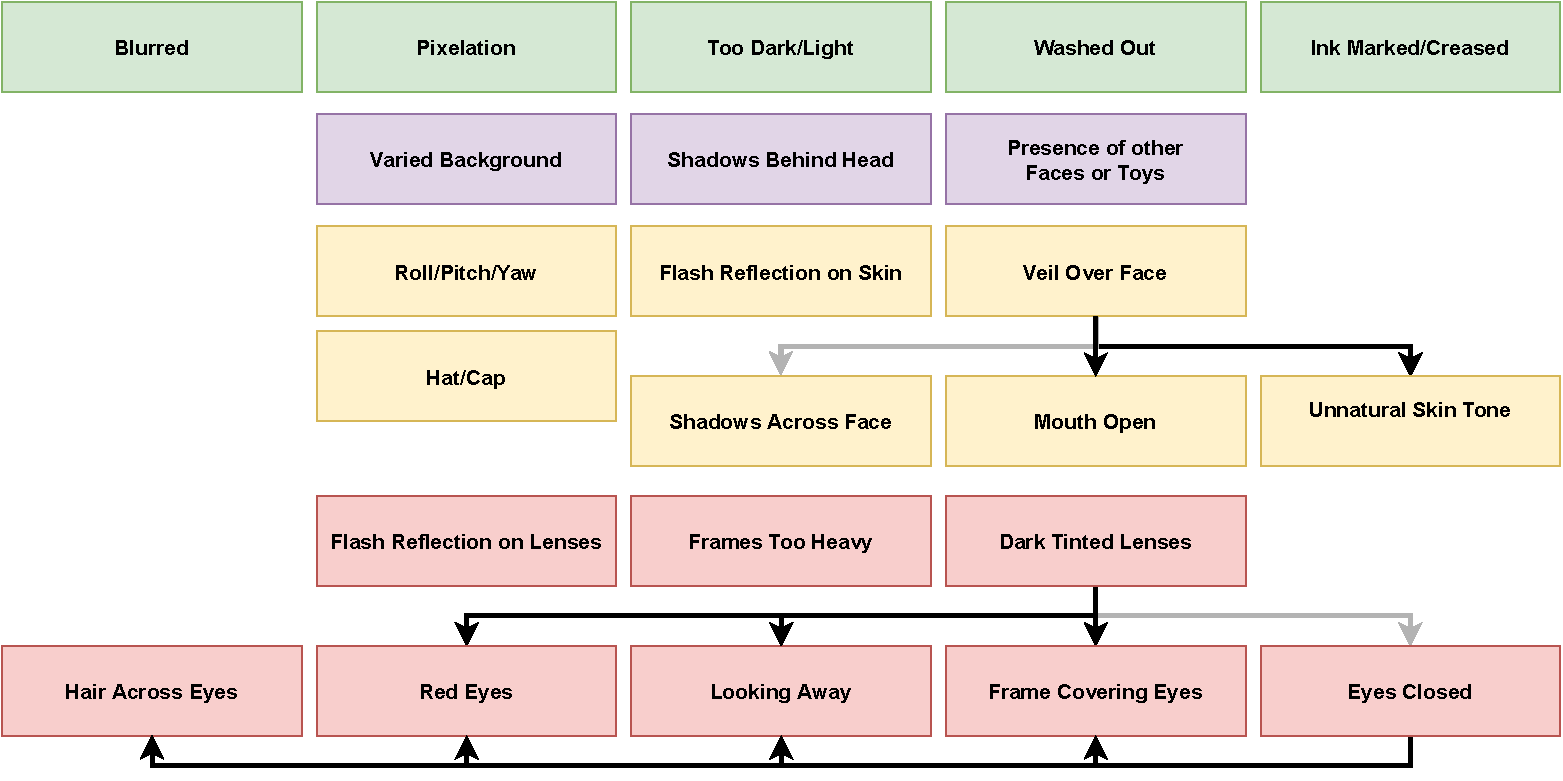
\includegraphics[width=\linewidth]{images/icao_dependencies.pdf}
\caption{Diagram of dependencies between non-compliant and dummy requirements. An arrow indicates that when the parent requirement is labeled as non-compliant, the children requirements are considered as dummy. A light gray arrow indicates that such relationship is not always true. Source: own elaboration.}
\label{fig:icao_dependencies}
\end{figure}

\subsubsection{Ad hoc Dataset}

 Usually, \acl{dl}-based methods require a large dataset for the learning process, primarily if the training is performed from scratch. Techniques like Transfer Learning or Data Augmentation can be employed in the case of low-size datasets. However, they presume some assumptions. For example, Transfer Learning works well when the original network was trained in a similar domain compared to the new problem. Likewise, to improve results with Data augmentation, we need to have significant intraclass variance in samples. Moreover, traditional Data Augmentation does not change the distributions of labels in a dataset since the random transformations are applied uniformly. 
 
 All these problems are presented in the \ficvtest dataset. First, the \icao standard represents a unique kind of problem and, thus, Transfer Learning may not be a valid option. Although some face datasets are available for research, Neural Networks are usually trained for face recognition in these datasets. Hence, while some features learned by these networks might be helpful for ICAO, some requirements are not popular in these databases (e.g., \citeReq{\inkmarked}) or are may be ignored by the network (like \citeReq{\variedbackground}). Finally, Data Augmentation might not help with the \ficvtest database due to the high level of unbalancing in some requirements. Also, some transformations applied by Data Augmentation procedures could affect part of the requirements. For example, random brightness may affect the  \citeReq{\toodarklight} requirement, and random rotations can change the angles of a face and disturb the \citeReq{\rollpitchyaw}.
 
 With only 571 images available of the \ficvtest database for all the 23 requirements, we resolved to increase the dataset by following a similar procedure adopted by the FICV. Therefore, we gathered more images from the AR, FRGC, and PUT databases. We also included images from the AFW database \citep{databaseAFW} and acquired new images regarding the \icao requirements. The images were annotated by three people specially trained for this task and double-checked by two experts. In total, we ended up with a training set with 5763 images. The image distribution per dataset is defined as follows:

\begin{itemize}
\item 22 images from AFW database of size from 362$\times$362 to 1984$\times$1984 pixels;
\item 1368 images from AR database;
\item 50 images from PUT database;
\item 1772 images from FRGC database; and
\item 2551 newly acquired images of size from 976$\times$1301 to 4608$\times$3456 pixels
\end{itemize}

Our dataset has 177 fully compliant images and 5568 images with one or more non-compliant requirements. One important detail to notice is that, although the ad hoc dataset has the label dummy in the ground truth, we decided to merge dummy and non-compliant labels. We did it for two reasons. First, according to the FICV protocol, only compliant and non-compliant images are considered for benchmark of each requirement (see section \ref{sec:fvcongoing} of Chapter \ref{sec:background}). Furthermore, the dataset imbalance is diminished by combining these two labels, and the intra-class variance of non-compliant images is increased. Therefore, it can help the network define a better decision boundary between compliant and non-compliant requirements and improve performance. Our tests corroborated such an effect. Finally, the distribution of labels per requirement can be seen in Table \ref{tab:req-dist}. 

% essa decisão foi uma consequencia da competicao. Em outro contexto, o dummy pode ser importante.

To better understand the ad hoc dataset, we performed some analysis of the images and labels. Such analyses are better described in the following subsection.

% Please add the following required packages to your document preamble:
% \usepackage{graphicx}
\begin{table}[tb]
\centering
\caption{Distribution of compliant (C) and non-compliant (NC) images for each requirement in the dataset. The last column indicates the proportion of NC images for the corresponding requirement.}
\label{tab:req-dist}
\begin{tabular}{clrrr}
\hline
\textbf{Req. \#} & \multicolumn{1}{c}{\textbf{Requirement description}} & \multicolumn{1}{c}{\textbf{C}} & \multicolumn{1}{c}{\textbf{NC}} & \multicolumn{1}{c}{\textbf{NC (\%)}} \\ \hline
\textbf{08} & Blurred & 4858 & 905 & 15.7\% \\
\textbf{09} & Looking away & 3946 & 1817 & 31.5\% \\
\textbf{10} & Ink marked/creased & 5742 & 21 & 0.3\% \\
\textbf{11} & Unnatural skin tone & 2540 & 3223 & 55.9\% \\
\textbf{12} & Too dark/light & 5307 & 456 & 7.9\% \\
\textbf{13} & Washed out & 5690 & 73 & 1.3\% \\
\textbf{14} & Pixelation & 5366 & 397 & 6.9\% \\
\textbf{15} & Hair across eyes & 4252 & 1511 & 26.2\% \\
\textbf{16} & Eyes closed & 4440 & 1323 & 22.9\% \\
\textbf{17} & Varied Background & 3248 & 2515 & 43.6\% \\
\textbf{18} & Roll/pitch/yaw & 4347 & 1416 & 24.6\% \\
\textbf{19} & Flash reflection on skin & 3143 & 2620 & 45.5\% \\
\textbf{20} & Red eyes & 4531 & 1232 & 21.4\% \\
\textbf{21} & Shadows behind head & 3866 & 1897 & 32.9\% \\
\textbf{22} & Shadows across face & 4621 & 1142 & 19.8\% \\
\textbf{23} & Dark tinted lenses & 5121 & 642 & 11.1\% \\
\textbf{24} & Flash reflection on lenses & 4584 & 1179 & 20.5\% \\
\textbf{25} & Frames too heavy & 5746 & 17 & 0.3\% \\
\textbf{26} & Frame covering eyes & 4084 & 1679 & 29.1\% \\
\textbf{27} & Hat/cap & 4914 & 849 & 14.7\% \\
\textbf{28} & Veil over face & 5399 & 364 & 6.3\% \\
\textbf{29} & Mouth open & 4231 & 1532 & 26.6\% \\
\textbf{30} & Presence of other faces & 5693 & 70 & 1.2\% \\ \hline
\end{tabular}%
\end{table}

\subsubsection{Ad Hoc Dataset Analysis}

The \autoref{fig:labels_by_sample} shows the number of images with 0 or more compliant/non-compliant labels in the ad hoc dataset. As pointed out earlier, there are 177 fully compliant images (i.e., the number of non-compliant labels equals zero). Also, we can notice that most images have 2 to 6 non-compliant requirements, but there are images with up to 14 non-compliant requirements.

\begin{figure*}
\centering
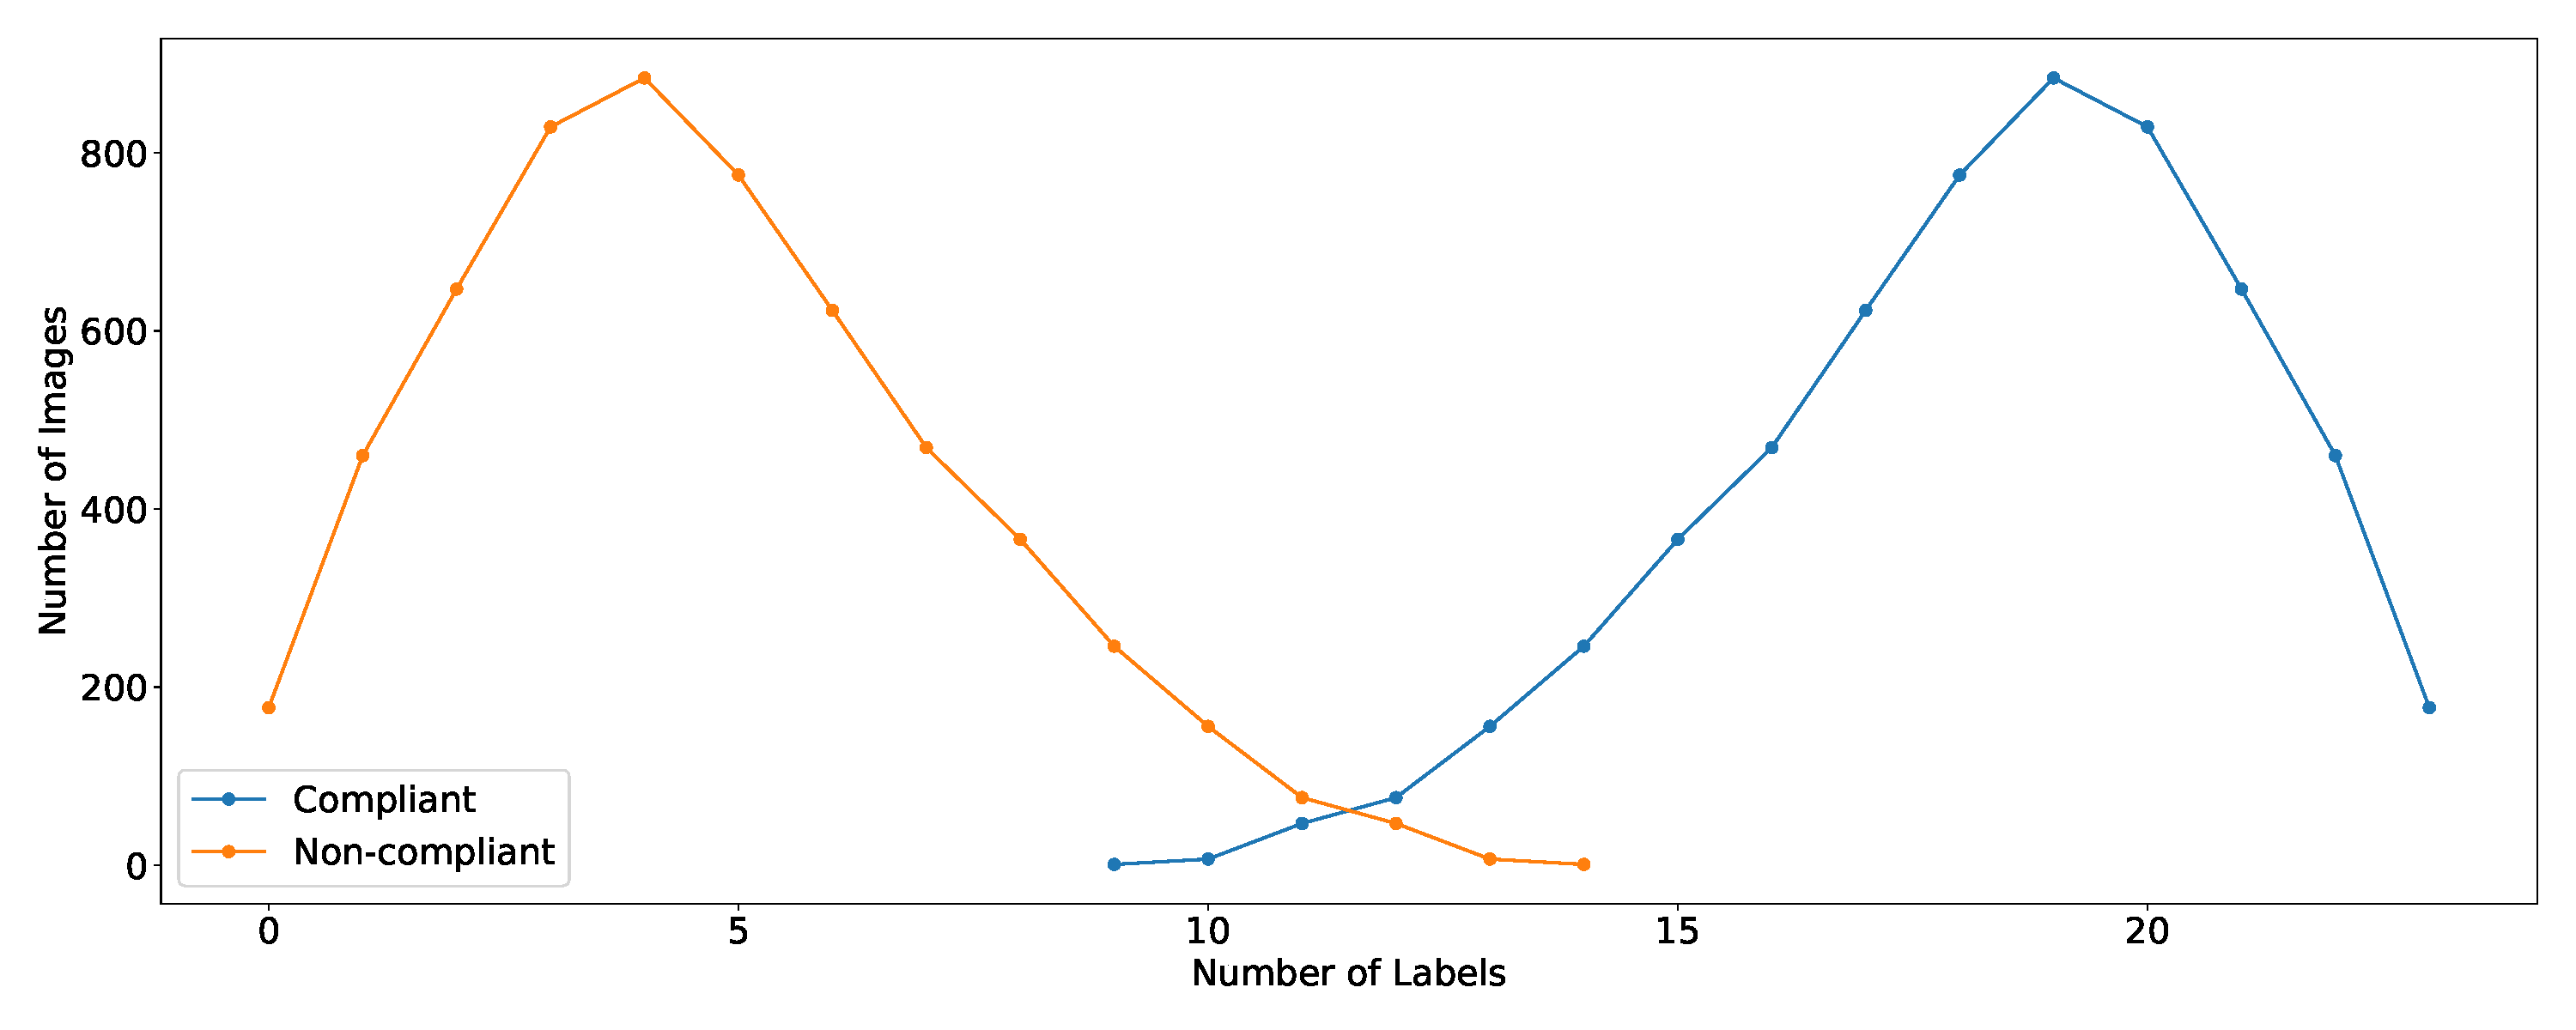
\includegraphics[width=\linewidth]{images/labels_by_sample.pdf}
\caption{Number of images according to the count of compliant/non-compliant labels. Source: own elaboration.}
\label{fig:labels_by_sample}
\end{figure*}

In \autoref{fig:reqs_distribution}, we can easily visualize the labels distribution by requirement presented earlier in \autoref{tab:req-dist}. As can be seen, the requirements \citeReq{\inkmarked}, \citeReq{\washedout}, \citeReq{\framestooheavy}, and \citeReq{\otherfacesortoys} are the most unbalanced ones. Also, the \citeReq{\unnaturalskintone} is the only requirement where the number of non-compliant samples is greater than the compliant.

\begin{figure*}
\centering
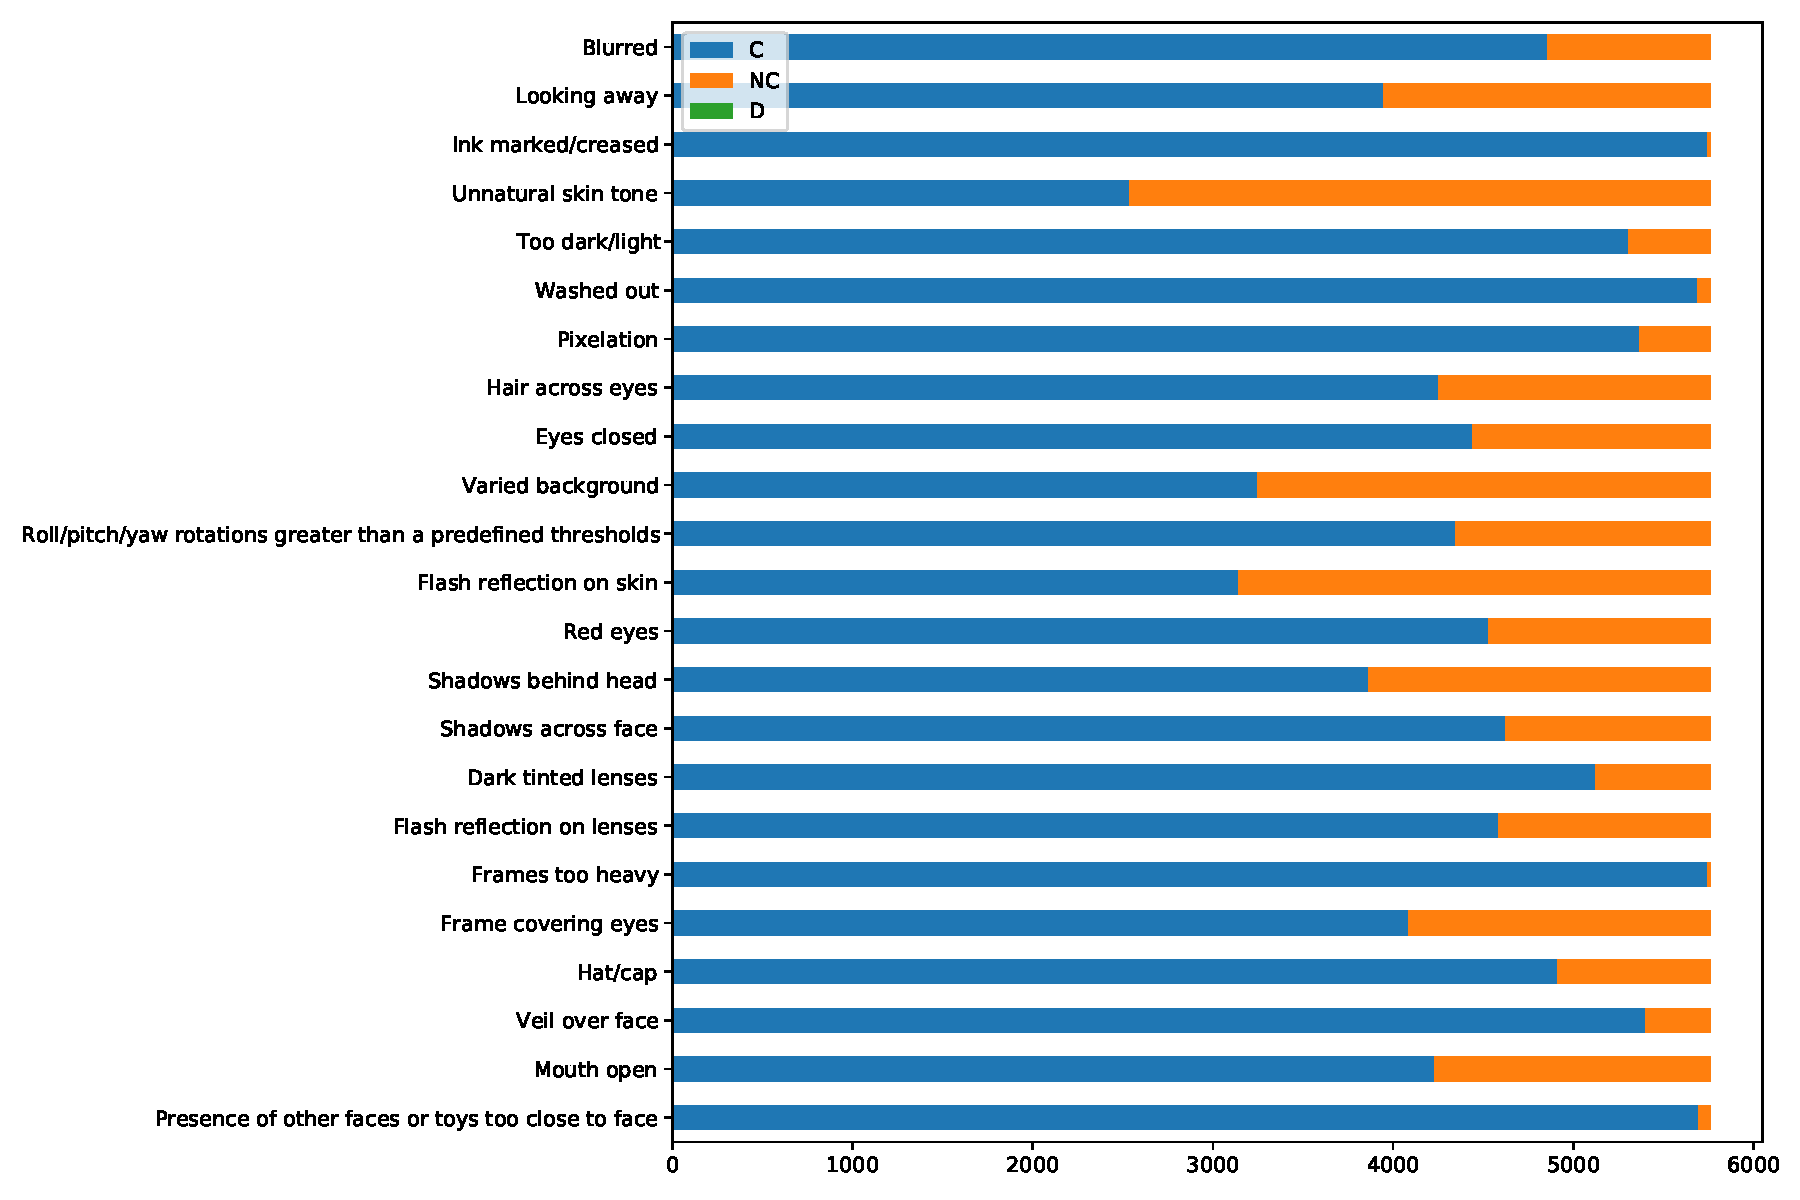
\includegraphics[width=\linewidth]{images/reqs_distribution.pdf}
\caption{Labels distribution per requirement. Source: own elaboration. Source: own elaboration.}
\label{fig:reqs_distribution}
\end{figure*}

The \autoref{fig:reqs_correlation} shows the correlation between non-compliant requirements. In other words, it measures how many images has two different non-compliant requirements occurring together. As expected, we can notice a strong correlation between eyes-related characteristics, e.g., \citeReq{\lookingaway}, \citeReq{\hairacrosseyes}, \citeReq{\eyesclosed}, \citeReq{\redeyes}, \citeReq{\darktintedlenses}, and \citeReq{\framecoveringeyes}. These are mainly caused by the dummy requirements that were converted to non-compliant. Moreover, considerable correlations can be observed between requirements associated to skin, for instance \citeReq{\unnaturalskintone} and \citeReq{\flashskin}. 

\begin{figure*}
\centering
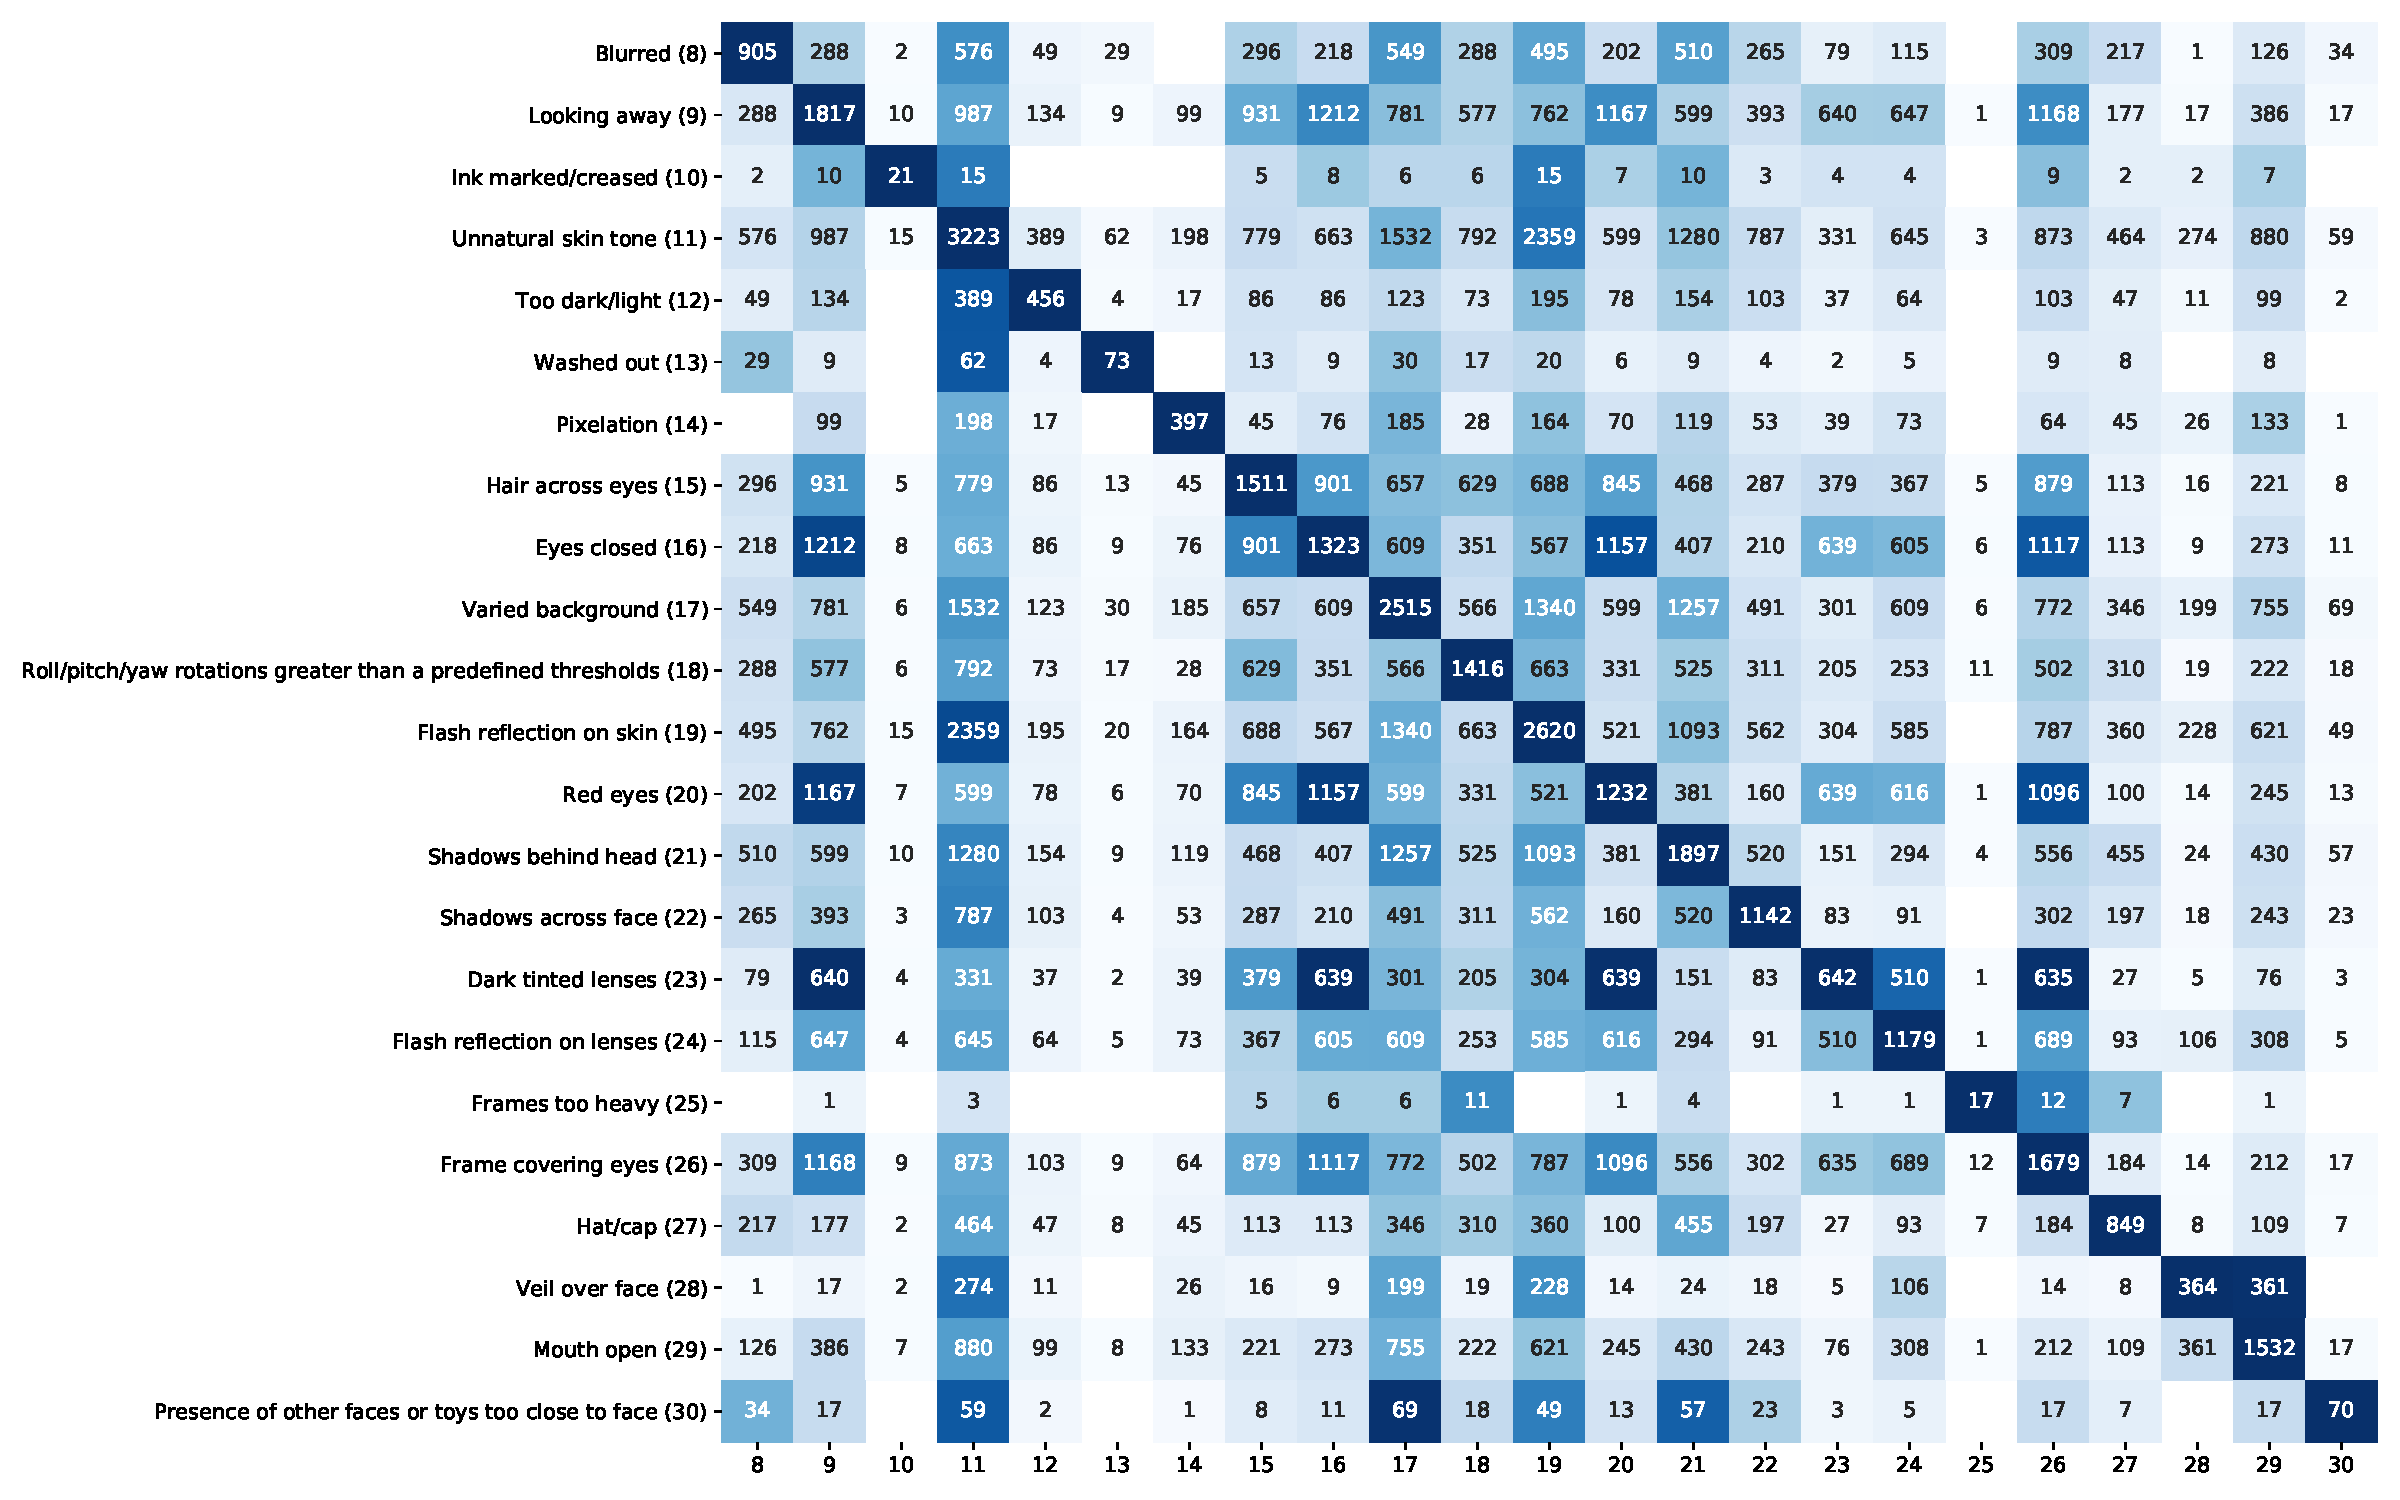
\includegraphics[width=\linewidth]{images/reqs_correlation.pdf}
\caption{Correlation between non-compliant requirements. Source: own elaboration.}
\label{fig:reqs_correlation}
\end{figure*}

According to our analysis, we came up with some conclusions. Firstly, since the dimensions of the images are different across the dataset, an approach to normalize images is required. It must avoid undesired normalization effects (like blur and pixelation) when possible and consider the trade-off between the input image quality and processing speed by the network. Regarding labels, the proposed method must consider the dataset unbalancing, and the most unbalance requirements might need special attention. Furthermore, the correlation between some requirements can be leveraged by a mechanism that shares features, like Autoencoders.

In the next section, we describe in detail the proposed method, called \methodname. It includes the architecture, the training process, as well the implementation details.

\subsection{\methodname}

\methodname is a \acl{dnn} developed to address the \icao standard. The architecture of \methodname is mainly based on Autoencoders. However, it is extended to apply a multi and collaborative learning approach. More details about the proposed method are described in the rest of this section. 

\subsubsection{Preprocessing} \label{sec:preprocessing}

Since the ad hoc dataset images have an extensive range of size dimensions (from 362$\times$362 to 4608$\times$3456), a preprocessing step was required to standardize the input image to \methodname. \autoref{fig:preprocessing} summarizes the preprocessing method applied in this work. A detailed explanation is provided as follows.

\begin{figure}
\centering
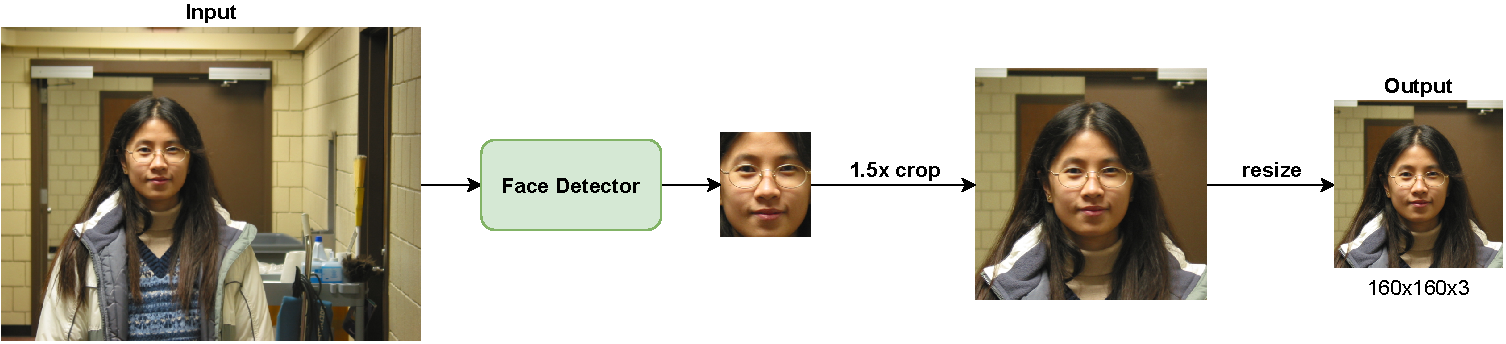
\includegraphics[width=\linewidth]{images/preprocessing.pdf}
\caption{Preprocessing step of \methodname. Source: own elaboration.}
\label{fig:preprocessing}
\end{figure}

The first step of our preprocessing method is face detection. We use a single shot multi-box detector based on MobileNet \citep{yeephycho} and trained on the WIDER FACE dataset \citep{yang2016wider}. This face detector has been chosen because it has a fair balance between speed and accurate results. According to our benchmarks, it was able to detect 98.99\% of all faces with an average of 1.6s per image in CPU. Moreover, this detector is compatible with TensorFlow 1.X versions used by the proposed method. 

Since the bounding box of the detected face is limited to the face region (from forehead to chin), we crop a squared region 1.5$\times$ larger than the detected face to include background and other relevant information to assess the requirements. Padded regions are filled with zeros because it generates less undesired artifacts than methods like border reflection, replication, or wrap. We do not apply any image normalization like illumination correction or rotation as it can affect requirements evaluation. 

Finally, the cropped image is resized to 160$\times$160 using the \texttt{INTER\_AREA} method of OpenCV\footnote{\url{https://docs.opencv.org/3.4/da/d54/group__imgproc__transform.html}}, since it is the recommended method for image decimation. Then, all pixels intensities are normalized to the $[0...1]$ range before feeding to \methodname. Again, the size of 160$\times$160 was chosen considering the trade-off between speed and results. More details are provided in Chapter \ref{sec:results}. 

\subsubsection{Architecture}

The overall architecture of \methodname can be seen in Figure \ref{fig:icaonet}. The architecture is composed of an Autoencoder in combination with a dense network branch. While the Autoencoder is employed for unsupervised learning of a highly discriminative embeddings space, the dense layer performs multi-label classification. 

\begin{figure*}
\centering
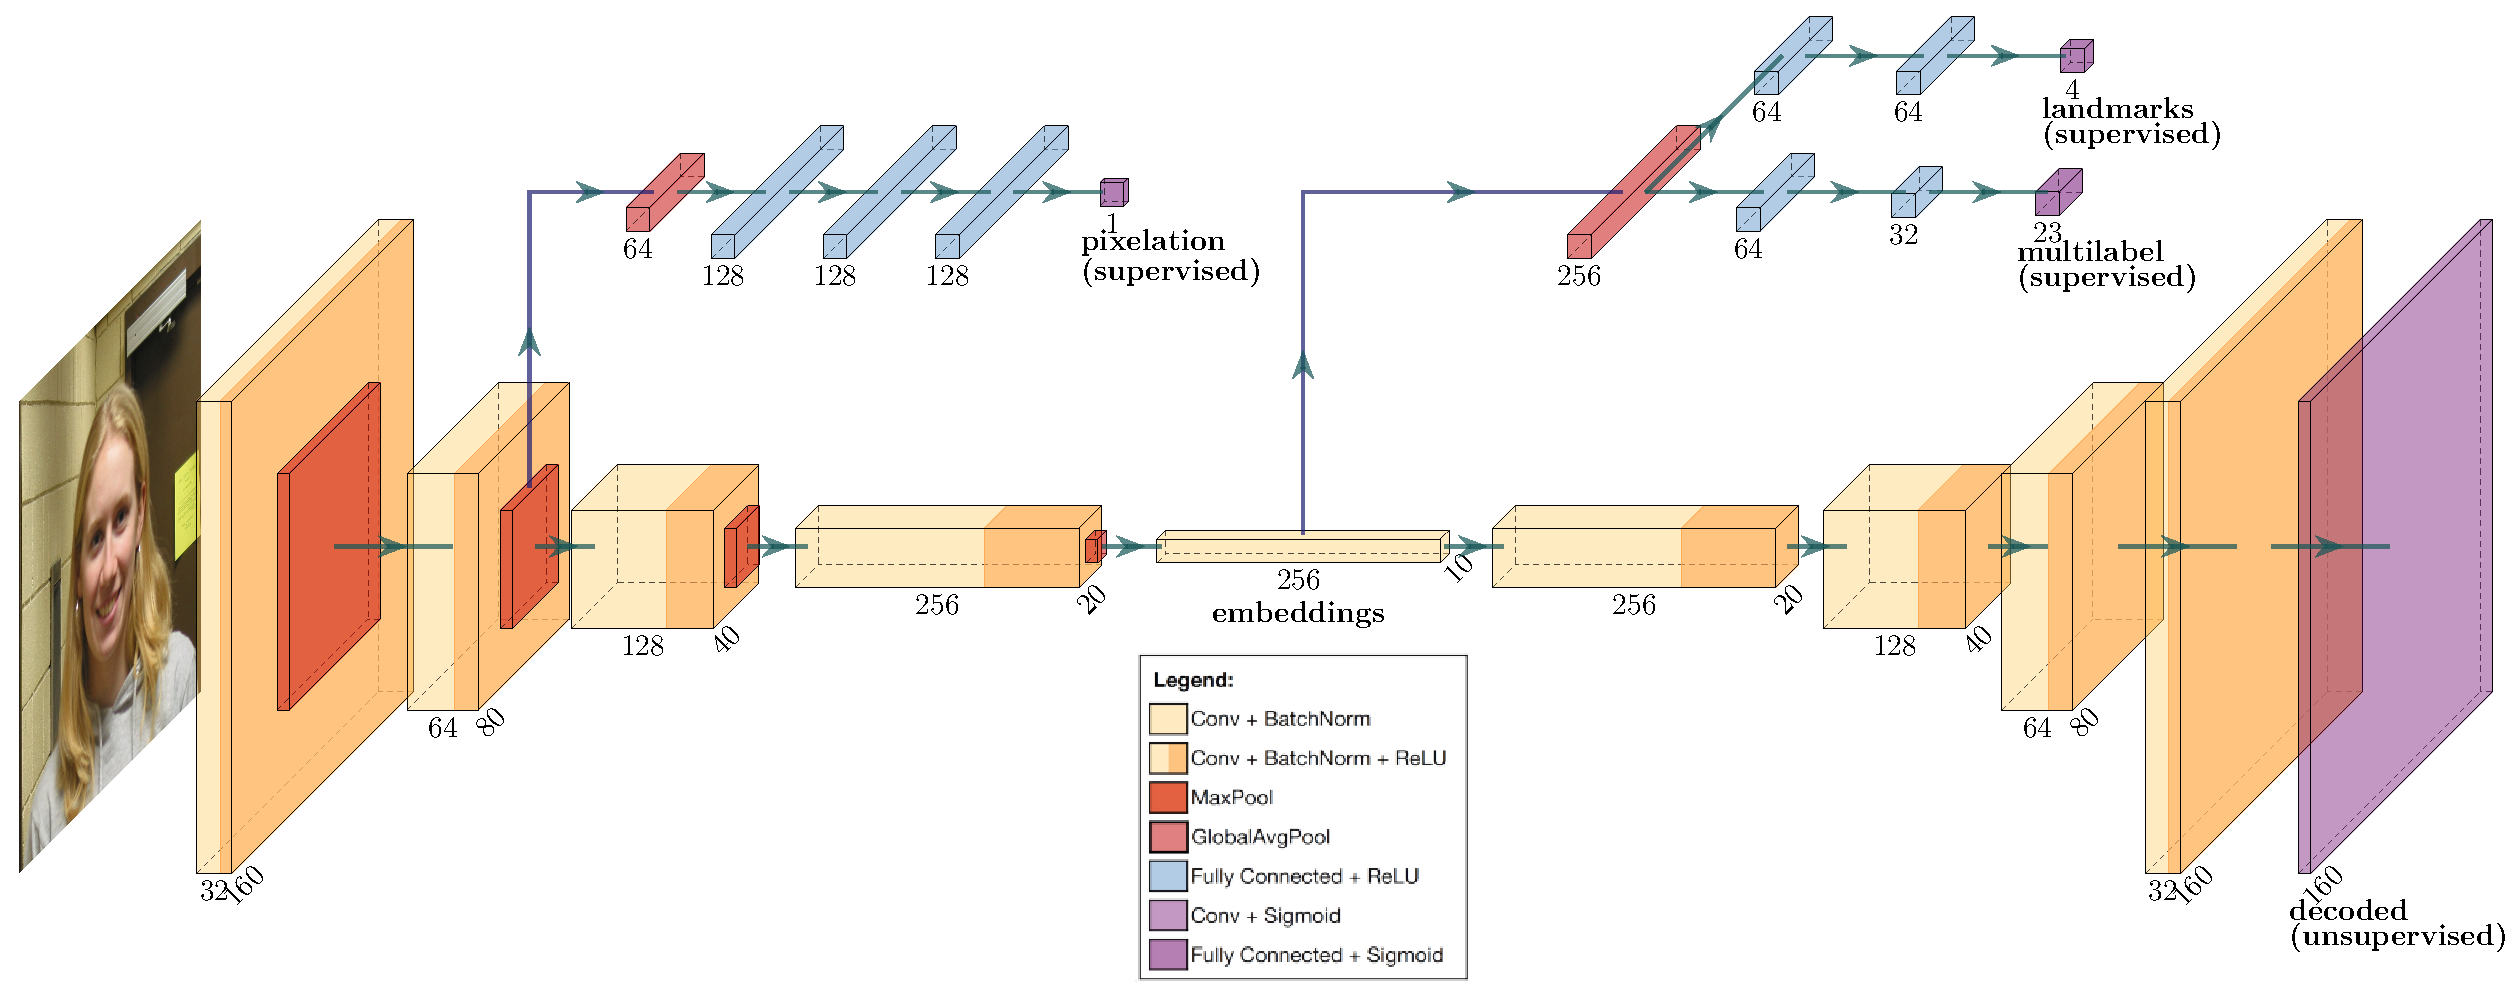
\includegraphics[width=\linewidth]{images/icaonet.pdf}
\caption{Architecture of \methodname. Source: own elaboration.}
\label{fig:icaonet}
\end{figure*}

The main idea behind the proposed architecture is to employ a multi and collaborative learning approach for the \icao requirements. It is multi-learning (also called multitasking) because the network solves both regression (image reconstruction) and multi-label classification (compliance prediction for each requirement) tasks at the same time. In contrast to \acfp{gan}, since both tasks are optimized together in training time, the learning process must also be collaborative. Hence, both branches must collaborate to learn an appropriate representation to solve both tasks. Additionally, we can assign different weights for each task to determine their importance during the optimization step (more details are given later).

The \methodname has three main components: (i) a \textbf{Shared Network} to compute shared embeddings; (ii) an \textbf{Unsupervised Branch} to perform image reconstruction; and (iii) a \textbf{Supervised Branch} for requirements assessment. Such components are detailed as follows.

\paragraph{Shared Network}

The top of the network is responsible for learning the embeddings shared by the unsupervised and supervised branches. These embeddings can be interpreted as a proper representation of the input and can be defined as an encoder function $h = f(x)$. Besides being used for dimensionality reduction, the shared embeddings are also used for feature learning in our network.

The architecture to compute the shared embeddings is based on the encoder component of Undercomplete Convolutional Autoencoder networks \citep{goodfellow2016deep}. The supervised branch receives a preprocessed input image of size 160x160 in the BGR color channel. Details of the preprocessing are given in section \ref{sec:preprocessing}. The first four convolutional layers are composed of 3x3 filters with batch normalization and ReLU activation. A 2D Max-pooling layer is applied for dimensionality reduction after each layer. The fifth layer is also composed of 3x3 convolutions with batch normalization. However, $tanh$ is used as a non-linear activation function instead of ReLU to normalize the embeddings values between -1 and 1. In our experiments, $tanh$ performed slightly better than ReLU for the encoded representations. The output of this layer stores the embeddings shared by the other branches. The embeddings are a 256-dimensional vector.

\paragraph{Unsupervised Branch}

This branch represents the decoder of an Autoencoder network. It is responsible for decoding the shared embeddings back to the original input. In mathematical terms, this branch will be responsible to learn the decoder function $\hat{x} = g(h)$, where $\hat{x}$ represents the reconstructed image. 

The architecture reflects the first four convolutional layers of the shared embeddings network. However, the Max-pooling layers are replaced by 2D Transposed Convolution layers. Furthermore, the last layer activation function is sigmoid since the input image pixels are normalized into the $[0...1]$ range. The shared embeddings network, together with the unsupervised branch, produces a full Convolutional Autoencoder Network \citep{goodfellow2016deep}.

The unsupervised branch uses the Mean Squared Error (MSE) to measure the image reconstruction task ($\mathcal{L}_1$), as defined by \autoref{eq:loss-unsupervised}:

\begin{equation}
\label{eq:loss-unsupervised}
\mathcal{L}_1 = \frac{1}{N} \sum_h^H \sum_w^W ({I_{h,w} - \hat{I}_{h,w}})^2
\end{equation}

\noindent where $N$ represents the number of pixels; $H$ and $W$, the image dimensions; $I$ and $\hat{I}$ are the input image and the reconstructed image, respectively. Since the same input image $I$ is used in the reconstruction task as ground-truth, this task is considered unsupervised (or semi-supervised). During training, the unsupervised branch will minimize the squared difference between the input image $I$ and the reconstructed image $\hat{I}$.

\paragraph{Supervised Branch}

This branch takes the shared embeddings as input and applies a fully connected network to perform multi-label classification. The first layer of this branch performs a GlobalAveragePooling to the shared embeddings. It transforms the 4-D dimensional vector of the embeddings into 2-D dimensions required by dense networks. We chose GlobalAveragePooling layers instead of Max Pooling layers since they are known to perform better in practice, as stated in \cite{zhou2016learning}. Then, there are two consecutive dense layers with 64 and 32 neurons, respectively. Dropout layers are included between each layer to prevent overfitting. Finally, the output layer has 23 neurons with sigmoid activation. Therefore, each neuron of the final layer outputs a normalized score between 0 and 1 for each corresponding requirement. In practice, the supervised branch's output is considered the likelihood of a given input image being compliant to each requirement of \icao standard.

We compute the Multi-label Cross-Entropy as the loss function for the supervised branch, defined by \autoref{eq:loss-supervised}:

\begin{equation}
\label{eq:loss-supervised}
\mathcal{L}_2 = \frac{1}{M} \sum_i^M {y_i \cdot log(\hat{y}_i)}
\end{equation}

\noindent where $M$ represents the number of requirements; $y_i$ is the ground-truth for each requirement (0: non-compliant, 1: compliant); and $\hat{y}_i$ is the predicted score for each requirement.

Since the network has two branches (supervised and unsupervised) and they are optimized using two different loss functions ($\mathcal{L}_1$ and $\mathcal{L}_2$), the final loss function $\mathcal{L}(I, \hat{I}, y, \hat{y})$ is defined by the \autoref{eq:loss-final}:

\begin{equation}
\label{eq:loss-final}
\mathcal{L}(I, \hat{I}, y, \hat{y}) = \lambda\mathcal{L}_1 + \gamma\mathcal{L}_2
\end{equation}

\noindent where $\lambda$ and $\gamma$ are two hyperparameters to control the trade-off between each loss function.

\subsubsection{Training} 

To train \methodname, the \ficvtest dataset is split into training and validation sets only. We consider the private dataset of the FICV competition (\ficvofficial) as the test set, and the benchmark results are reported as our final results. Both training and validation sets are randomly divided using a stratified multi-label approach. Thus, the compliant and non-compliant proportions seen in Table \ref{tab:req-dist} are preserved. Approximately 10\% of the dataset (580 images) is used as the validation set, while the remaining images are selected for network training.

Regarding the architecture, since most of the \methodname structure is based on undercomplete Autoencoders, there was no need to employ many regularization techniques during training. However, we still apply batch normalization before activation functions in the Convolutional layers and Dropouts in some dense layers of the supervised branch. The Early Stopping technique is also employed to prevent overfitting, and the patience hyperparameter is based on the \acl{mcc}, as presented in \autoref{eq:mcc}. The MCC was chosen because it is a robust metric for unbalanced datasets (see section \ref{sec:mcc} of Chapter \ref{sec:background}) and it performed better than \acs{eer} in our experiments. All metrics described in section \ref{sec:measures} of Chapter \ref{sec:background} are evaluated at the end of each epoch and will be reported in the results chapter.

The network is written in Python using Keras\footnote{\url{https://keras.io}} framework (v2.3.1) with TensorFlow (v1.13.1) backend. The Mlflow\footnote{\url{https://www.mlflow.org}} library (v1.7.0) is used for experiments tracking/comparison and logging of hyperparameters, metrics, and artifacts. The source code, along with the trained network, can be found in Github\footnote{\url{https://github.com/arnaldog12/doutorado}}. Furthermore, the experiments are conducted in a Windows 10 machine with Intel\textsuperscript{\tiny\textregistered} Core\textsuperscript{\tiny\texttrademark} i5-8300H of 8\textsuperscript{th} generation, 16 GB of DDR4 2666MHz RAM, SSD of 512 GB, and NVIDIA\textsuperscript{\tiny\textregistered} GeForce\textsuperscript{\tiny\textregistered} GTX 1050 with 4GB of RAM.

One last important detail about \methodname training is that we took special care over the experimentation phase. For example, we set the random seed of Python, its \texttt{random} module\footnote{\url{https://docs.python.org/3/library/random.html}}, and Numpy\footnote{\url{https://numpy.org}} and TensorFlow libraries to be the same for all experiments. It assures reproducibility and ensures that the best results of current experiments are not achieved by chance.

\subsubsection{Parameters and Hyperparameters} \label{sec:hyperparams}

The base architecture of \methodname -- composed of the three components described earlier (shared network, supervised branch, and unsupervised branch) -- contains a total of 1,980,890 parameters. From these parameters, 1,978,458 are trainable, and the remaining 2,432 are non-trainable parameters related to the mean and variance computed by batch norm layers. In terms of size, the \methodname occupies 22.8 MB in the disk when stored as a \texttt{.hdf5} file.

One important detail to mention about the proposed architecture refers to the unsupervised branch, which is used during training only. Once the network is trained, the unsupervised branch is detached from the model as the reconstruction task is not valuable for ICAO assessment and can be ignored. In this case, the number of parameters is reduced to 1,000,727. Furthermore, after model \textit{freezing}\footnote{Freezing is a typical operation in Keras/TensorFlow models. It removes unnecessary data for prediction from the model file, e.g., the optimizer, metrics, metadata, gradients, and many others.}, the model size is reduced to only 3.83 MB in the disk. It helps speed up the running time considerably.

The \methodname was trained by 100 epochs and a batch size of 32. All layers are randomly initialized by Xavier initialization \citep{glorot2010understanding}. To prevent overfitting and improve generalization, we use Early Stopping with 30 epochs of patience. In layers where Dropout is applied, we keep 50\% of neurons. The Adaptive Momentum Estimation (Adam) is applied as optimizer with learning rates $\alpha=10^{-3}$, $\beta_1=0.9$, $\beta_2=0.999$, and $\epsilon=10^{-7}$. For the loss function (\autoref{eq:loss-final}), we use $\lambda=1.0$ and $\gamma=2.0$.

\section{Preliminary Evaluations} \label{sec:results}

This chapter presents and discusses the preliminary results accomplished by the proposed method so far. First, \methodname results in the training stage are presented, including the loss and metrics computed. Secondly, we discuss the performance of the proposed method in the FICV competition. Then, the \methodname is compared against the best results achieved by the methods shown in Chapter \ref{sec:literature}. Finally, we analyze some visualizations performed over the proposed method to understand its predictions.

\subsection{Training Performance}

In this subsection, we discuss the training performance regarding the \icao requirements followed by the results of eye landmarks detection. We focus on analysing  the loss charts and values of metrics described in Chapter \ref{sec:measures}.

\subsubsection{Requirements}

We start by presenting the results of \methodname during the training phase. The \autoref{fig:losses} shows the loss in training and validation sets for unsupervised and supervised branches individually. As can be seen, the loss of unsupervised branch was lower and smoother than the supervised during the whole training. This behaviour was expected since (i) the reconstruction task performed by the unsupervised branch is theoretically more straightforward than the multi-label classification carried out by the supervised branch, and (ii) the unsupervised loss has a higher weight during training (see section \ref{sec:hyperparams} and \autoref{eq:loss-final}). 

A more detailed analysis of our loss curves shows that \methodname presented an appropriate balance between bias and variance. In the unsupervised branch, both train and validation loss are approximately zero and similar to each other. Therefore, the network achieved a notable performance in reconstructing the input image from the shared embeddings. Similarly, even though the losses from the supervised branch are more significant than the unsupervised one, they are still close to zero. However, we can notice a noisier loss curve regarding the validation set. Although such loss curves present a higher variance, they keep near the training curve through the epochs. Furthermore, the overfitting was prevented by the regularization techniques employed during training, i.e., batch normalization, dropout layers, Early Stopping, and the architecture itself (as detailed in Section \ref{sec:hyperparams}).

\begin{figure}[ht]
\centering
\subfigure[unsupervised]{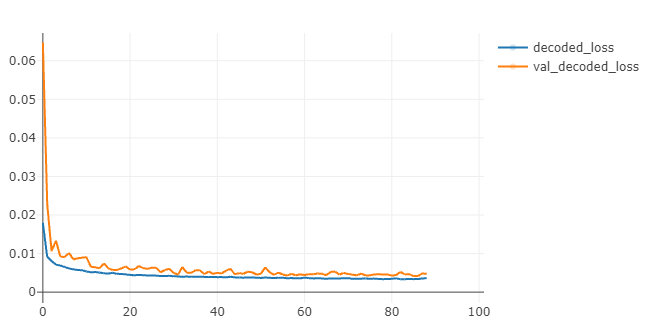
\includegraphics[width=0.8\linewidth]{images/graphs/loss_unsupervised.png}}
\hfill
\ContinuedFloat
\subfigure[supervised]{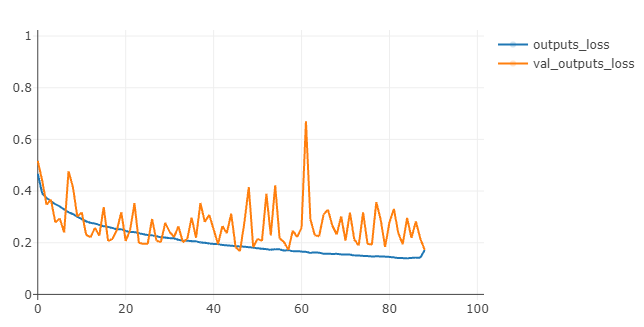
\includegraphics[width=0.8\linewidth]{images/graphs/loss_supervised.png}}
\caption{Loss of training and validation sets for (a) unsupervised and (b) supervised branches. Source: own elaboration.}
\label{fig:losses}
\end{figure}

The final metrics of \methodname are given in \autoref{tab:metrics}, where some meaningful insights about the proposed method can be observed. First, it is better to predict the compliant requirements (positive class) than the non-compliant since the Precision and Recall are higher than the \acs{npv} and Specificity. Probably, this is influenced by the unbalanced dataset. Moreover, the \acl{fp} predictions (type-I error) are a more critical problem of \methodname because both Recall and \acs{npv} are greater than Precision and Specificity, respectively. In particular, the Specificity indicates that a reasonable amount of non-compliant requirements are being assigned as compliant. On the other hand, the proposed method achieved considerably high values of F-measure and F-beta, which shows a fair balance between Precision and Recall. Finally, the notable \acs{mcc} score (82.78) indicates that the \methodname was able to learn valuable patterns for both compliant/non-compliant requirements even with the unbalancing present in the \adhoc database.

\begin{table}[H]
\centering
\caption{Global metrics of \methodname achieved in the best training epoch.}
\label{tab:metrics}
\begin{tabular}{@{}cc@{}}
\toprule
\textbf{Metric} & \textbf{Value (\%)} \\ \midrule
Accuracy & 94.27 \\
Precision & 94.53 \\
Recall & 97.89 \\
F-measure & 96.15 \\
F-beta & 97.14 \\
NPV & 91.67 \\
Specificity & 81.69 \\
MCC & 82.78 \\ \bottomrule
\end{tabular}
\end{table}

\subsubsection{Eye Location Accuracy} \label{sec:eye_location_acc}

In contrast to the intuition, the detection of eye landmarks revealed to be a harder task than the assessment of \icao requirements. The \autoref{fig:eye-training} presents the Wing loss and eye location accuracy ($d_{eye} \in [0;0.1[$) in training and validation sets. In contrast to the supervised branch for requirements, we can notice the presence of bias in the loss graph during training (the loss is far away from zero), indicating the network was not able to learn useful patterns and detect eye landmarks accurately. Such behaviour also happens in the validation set. Nonetheless, these results also reflect in the eye location accuracy metric, which reach the maximum value of $46.18\%$ in the \adhoc dataset. 

\begin{figure}[ht]
\centering
\subfigure[Wing Loss]{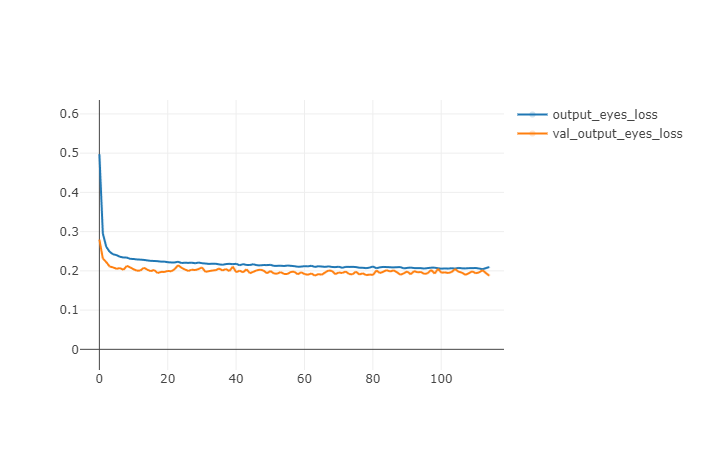
\includegraphics[width=0.8\linewidth]{images/graphs/loss_eyes.png}}
\subfigure[Eye Localization Accuracy]{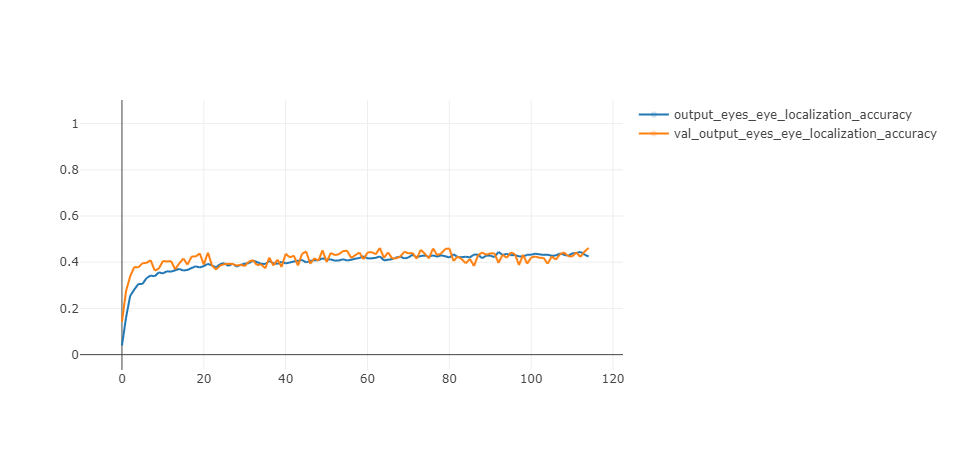
\includegraphics[width=0.8\linewidth]{images/graphs/eyes_location_accuracy.png}}
\caption{Results of eye localization for training and validation sets: (a) wing loss and (b) $d_{eye} \in [0;0.1[$. Source: own elaboration.}
\label{fig:eye-training}
\end{figure}

A sample of images with the landmarks predicted by \methodname is shown in \autoref{fig:eyes_detection}. In the first two rows, there are arbitrary examples of most precise detections (i.e., $d_{eye} \in [0;0.1[$). We can observe that \methodname can perform accurate detections for frontal face images even with the presence of requirements that could potentially harm accurate localization of the landmarks. For example, we can see the presence of images with \framecoveringeyes and \toodarklight. On the other hand, in the last two rows, there are samples of the worst detections, i.e. $d_{eye} \geq 0.3$. In this case, an evident pattern of highly rotated face images (\rollpitchyaw) is perceptible. Furthermore, the presence of other requirements can be noticed (e.g, \blurred and \framestooheavy).

\begin{figure}[h]
\centering
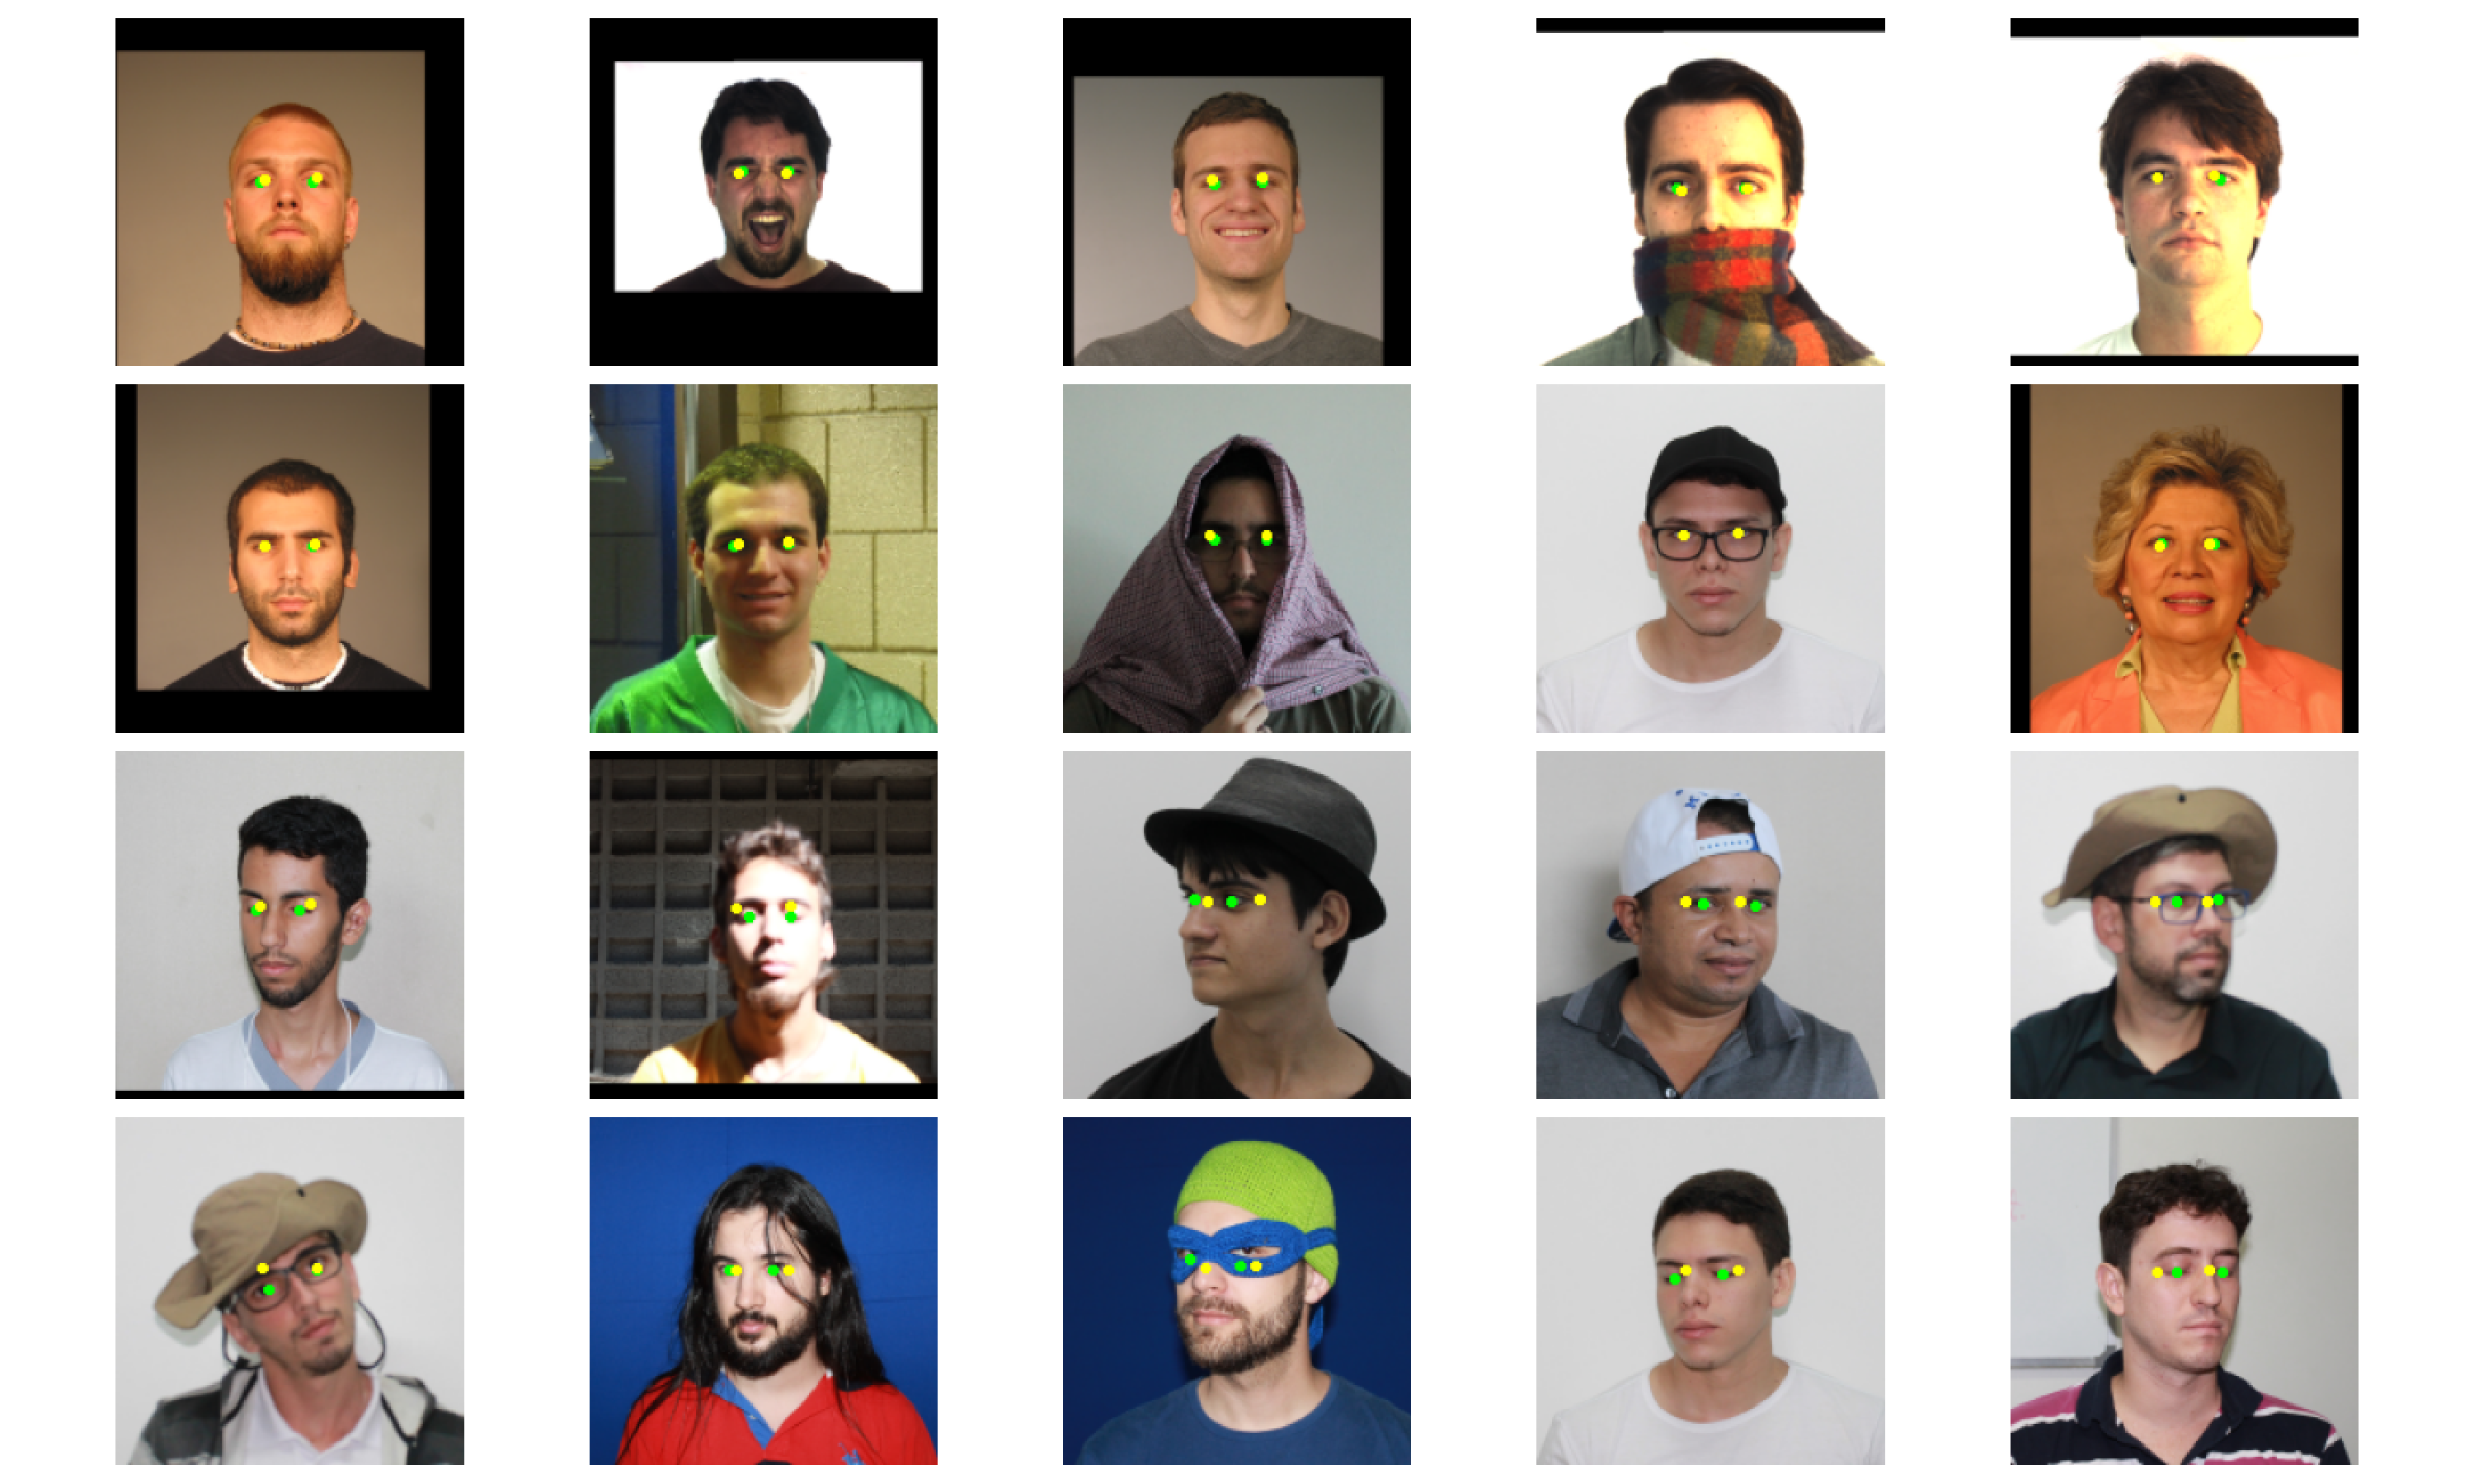
\includegraphics[width=\linewidth]{images/eyes/detections.pdf}
\caption{Results of eyes landmarks detection by \methodname. The first two rows contains images with $d_{eye} \in [0;0.1[$, and the last rows are for $d_{eye} \geq 0.3$. The ground-truth annotations are shown in green, while network predictions are in yellow.}
\label{fig:eyes_detection}
\end{figure}

We analysed the network predictions for eye landmarks to understand the bias observed during training. In \autoref{fig:heatmap_eyes}, we can see a heatmap of landmarks in the validation set. As can be noticed, there are two noticeable clusters for each eye, indicating that the networks is essentially predicting landmarks over the same regions regardless the input image. We suppose this behaviour is caused mainly by the preprocessing step, which centers the face in the input image.

Moreover, we presume the low performance in eye landmark localization can be explained by one or more reasons from below:

\begin{figure}[h]
\centering
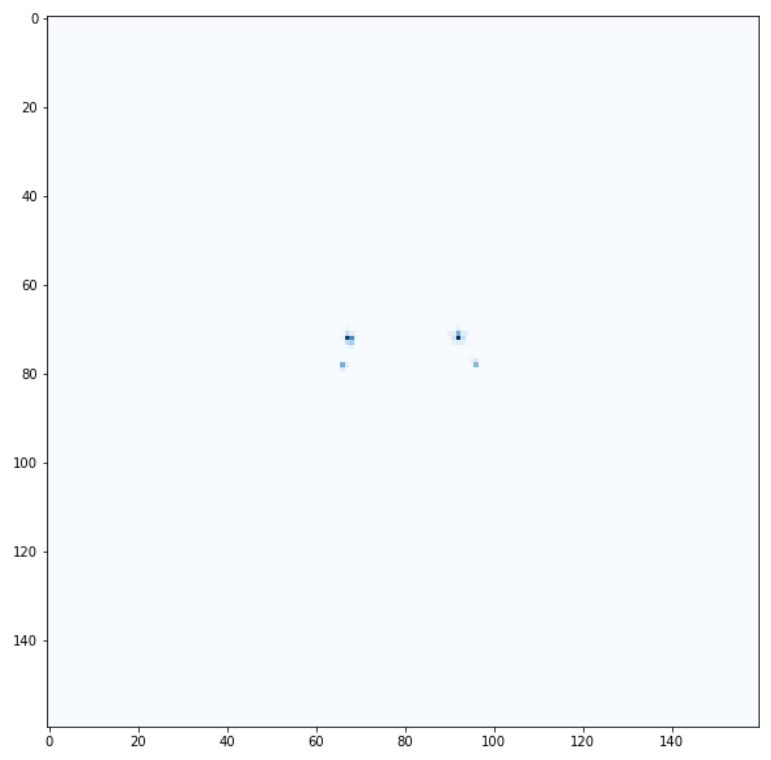
\includegraphics[width=0.6\linewidth]{images/eyes/heatmap_eyes_v0.914.png}
\caption{Heatmap of detected eye landmarks in the \adhoc dataset.}
\label{fig:heatmap_eyes}
\end{figure}

\begin{enumerate}[i]
\item \textbf{Preprocessing}: our preprocessing method centralize the face by creating a region around it (see Section \ref{sec:preprocessing}). Therefore, the network can be inducted to predict the mean of landmark positions to minimize the loss function. However, we tried to apply different levels of image augmentation in other experiments. Although the predictions were more distributed over the image, there was no significant changes in the loss and location accuracy.

\item \textbf{Dataset}: our \adhoc image dataset is mostly composed by images with frontal faces with little variation in face poses and alignment. In addition, the amount of images (approximately five thousand) is noticeably low in comparison with other landmarks datasets. For example, there are more than 200 thousand images with labeled landmarks in the 300-VW \citep{tzimiropoulos2015project} or CelebFaces \citep{yang2015facial} datasets. In fact, we ran some experiments with a subset of CelebFaces dataset as our training set (and left the entire \adhoc dataset as validation). In all of them, overfitting was achieved (i.e., high performance in training, but low performance in validation). We believe it comes from the fact that the patterns found in CelebFaces dataset are even easier than in ours. All faces are centered and with corrected orientation (the last is not carried out by our preprocessing step). Again, as mentioned before, we tried data augmentation, but it did not help to improve overall performance.

\item \textbf{Embeddings}: when training the branch for detection of eye landmarks, the remaining parts of \methodname architecture was frozen, including the encoder and corresponding embeddings. We could argue that (i) the embeddings does not contain helpful representation of the eyes that can be relevant for landmark detection; and (ii) it can be harmful to the landmarks branch since it would not have the chance to update the embeddings. Despite of it, we already had empirical evidence that the embeddings contains useful information of the eyes before training the landmarks branch. Later is this work, we will see the regions closer to eyes are important for requirements assessment (see Section \ref{sec:netviz}).

\item \textbf{Training Components}: we ran tests with \acs{mse}, Wing Loss, and $d_{eye}$ as both loss functions and metrics for early stopping.  After all, \methodname was not able to predict the landmarks accurately. It goes against to other works found in the literature that also applies multitask learning for facial landmarks prediction (e.g., \citep{zhang2014facial, ranjan2017hyperface, zhang2015learning}. On the other hand, we could have leveraged the use of more advanced losses and models. It will be left for future works though.

\end{enumerate}

In conclusion, considering the scope of the possible reasons mentioned above, we suspect the dataset is the main problem for the low performance on eye localization accuracy. Therefore, by improving the data with more variations in face pose, location and orientations, the results may be improved. Nevertheless, further investigation must be conducted to verify this hypothesis.


\subsection{Results in the FICV Competition} \label{sec:ficv_results}

In \autoref{tab:icaonet-ficv}, we can see the \acl{eer} and Rejection Rate for each FICV dataset. In the \ficvtest, the method proposed was able to achieve a perfect \acs{eer} in eight requirements (08, 11, 12, 16, 23, 24, 28, and 29). In the \ficvofficial dataset, it happened only in the \veiloverface, even though most of the other results are considerably low. 

\begin{table}[tb]
\centering
\caption{Results of \methodname according to the benchmark of the FICV competition. The EER and Rejection Rate are shown in percentage.}
\label{tab:icaonet-ficv}
\begin{tabular}{@{}clrrrr@{}}
\toprule
\multirow{2}{*}{\textbf{Req. \#}} & \multicolumn{1}{c}{\multirow{2}{*}{\textbf{Requirement description}}} & \multicolumn{2}{c}{\textbf{FICV-TEST}} & \multicolumn{2}{c}{\textbf{FICV-1.0}} \\ \cmidrule(l){3-6} 
 & \multicolumn{1}{c}{} & \multicolumn{1}{c}{EER} & \multicolumn{1}{c}{Rej.} & \multicolumn{1}{c}{EER} & \multicolumn{1}{c}{Rej.} \\ \midrule
\textbf{08} & Blurred & 0.00 & 0.00 & 2.10 & 0.60 \\
\textbf{09} & Looking away & 5.00 & 0.00 & 5.40 & 0.00 \\
\textbf{10} & Ink marked/creased & 46.70 & 0.00 & 49.00 & 0.00 \\
\textbf{11} & Unnatural skin tone & 0.00 & 0.00 & 1.70 & 0.00 \\
\textbf{12} & Too dark/light & 0.00 & 0.00 & 1.20 & 0.00 \\
\textbf{13} & Washed out & 1.50 & 0.00 & 7.30 & 0.00 \\
\textbf{14} & Pixelation & 26.70 & 0.00 & 29.00 & 0.00 \\
\textbf{15} & Hair across eyes & 4.50 & 0.00 & 13.70 & 0.40 \\
\textbf{16} & Eyes closed & 0.00 & 0.00 & 0.80 & 0.00 \\
\textbf{17} & Varied Background & 1.00 & 1.00 & 8.40 & 1.30 \\
\textbf{18} & Roll/pitch/yaw & 2.00 & 0.00 & 4.60 & 0.20 \\
\textbf{19} & Flash reflection on skin & 2.10 & 2.00 & 1.00 & 0.00 \\
\textbf{20} & Red eyes & 6.90 & 1.70 & 8.20 & 1.50 \\
\textbf{21} & Shadows behind head & 2.90 & 0.00 & 3.30 & 0.00 \\
\textbf{22} & Shadows across face & 2.00 & 0.00 & 3.30 & 0.20 \\
\textbf{23} & Dark tinted lenses & 0.00 & 0.00 & 0.40 & 0.00 \\
\textbf{24} & Flash reflection on lenses & 0.00 & 1.00 & 0.80 & 0.00 \\
\textbf{25} & Frames too heavy & 9.10 & 0.00 & 9.50 & 0.00 \\
\textbf{26} & Frame covering eyes & 1.50 & 0.00 & 2.30 & 0.60 \\
\textbf{27} & Hat/cap & 3.10 & 0.00 & 5.70 & 0.20 \\
\textbf{28} & Veil over face & 0.00 & 1.00 & 0.00 & 0.00 \\
\textbf{29} & Mouth open & 0.00 & 0.00 & 2.30 & 0.00 \\
\textbf{30} & Presence of other faces & 41.00 & 0.00 & 41.40 & 0.00 \\ \bottomrule
\end{tabular}
\end{table}

Three requirements had an \acs{eer} greater than 40\% (10, 14, and 30) in both datasets. In common, they all have a high level of unbalancing (as presented in \autoref{tab:req-dist}). However, other requirements with similar or even worse unbalancing achieved better performance (e.g., 25, 13, or 28). In the case of \pixelation, we credit this bad result to the preprocessing since some high-resolution images are pixelated after the resizing step. Moreover, to easily improve the results of the \otherfacesortoys, we could automatically decrease the score of images with two or more detected faces by our detector. However, the development of post-processing methods is not the primary objective of this work, but it could be considered a future work or be released in the next versions of \methodname.

In terms of Rejection Rates, only four requirements had images rejected during evaluation (08, 15, 17, and 18). According to our implementation, we only reject images for evaluation when a face is not detected. Therefore, such rejections represent the false negatives from the face detector used to preprocess input images (see section \ref{sec:preprocessing} of Chapter \ref{sec:method}). Furthermore, by analyzing these requirements, all of them may hamper face detection in extreme cases. 

We highlight the substantial differences in \acs{eer} between both datasets in \autoref{tab:icaonet-ficv} for requirements 13, 15, and 17. In the case of \washedout, we believe it is caused because all the non-compliant images of this requirement in the \ficvtest belong to the AR database (see \autoref{fig:washedout}). Therefore the pattern learned by the network might not have been generalized to the official database. For the \variedbackground requirement, it may be affected by the cropping applied during preprocessing step of our method (see \autoref{fig:preprocessing}). The cropping can either (i) generate black borders to the input image or (ii) exclude artifacts that introduce variability to the background. According to our analysis to understand our network's output, we could observe that the black borders do not substantially influence the predictions (more details are provided further in section \ref{sec:netviz}). Thus, as can be seen in \autoref{fig:variedbgd}, the artifacts excluded by crop can have a noticeable effect on network learning. Lastly, one possible reason for the \hairacrosseyes requirement can be the resizing operation performed by the preprocessing step (see \autoref{fig:hairacrosseyes}). Since the \adhoc dataset images are mostly of high resolution and they are reduced to 160x160, it can affect the images where thin locks of hair are crossing the eyes region. These cases are not rare to occur in the dataset and, even using the recommended method for image decimation (see section \ref{sec:preprocessing}), the resize may be contributing negatively to the patterns of this requirement. 

\begin{figure}[t]
\centering
\subfigure{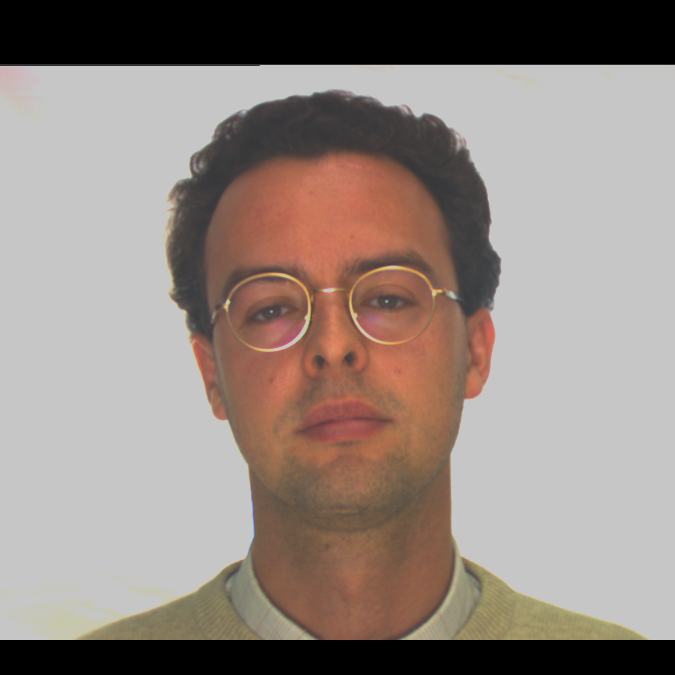
\includegraphics[width=0.23\linewidth]{images/washed_out/AR_m-007-1_C40.png}}
\hfill
\subfigure{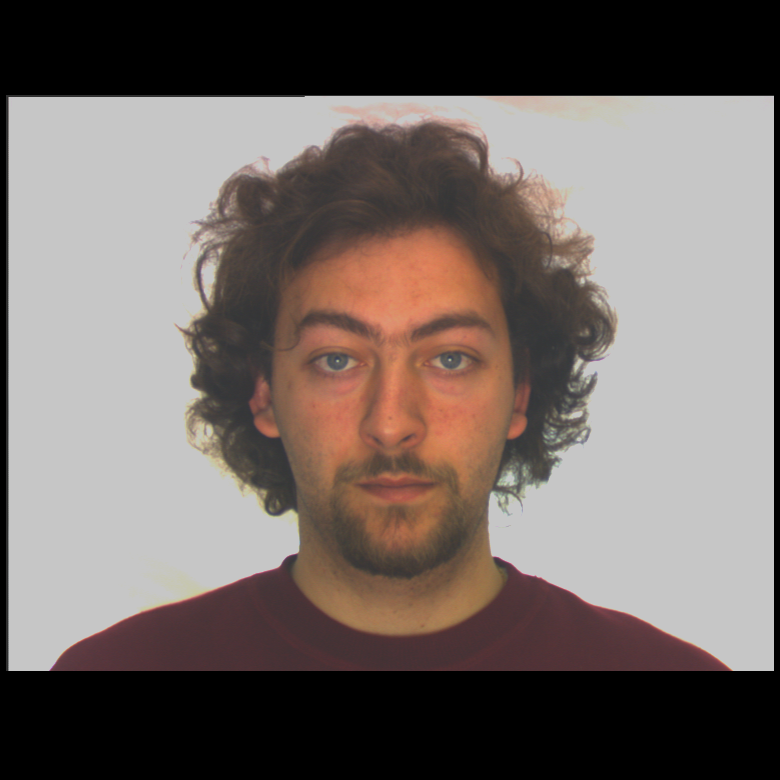
\includegraphics[width=0.23\linewidth]{images/washed_out/AR_m-048-1_C40.png}}
\hfill
\subfigure{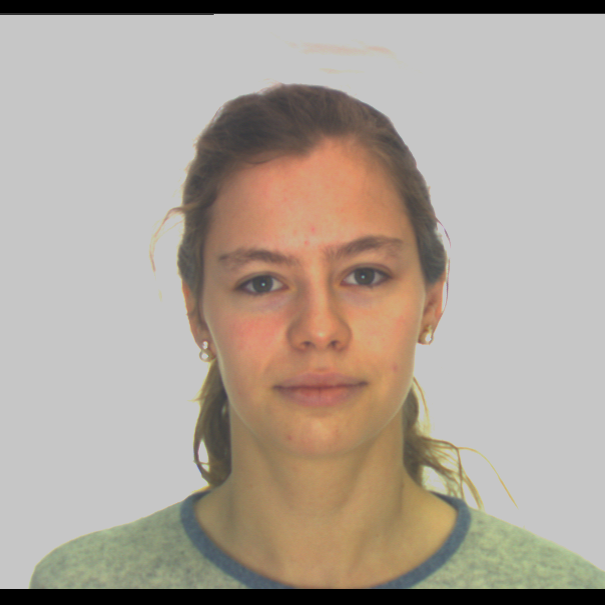
\includegraphics[width=0.23\linewidth]{images/washed_out/AR_w-018-1_C40.png}}
\hfill
\subfigure{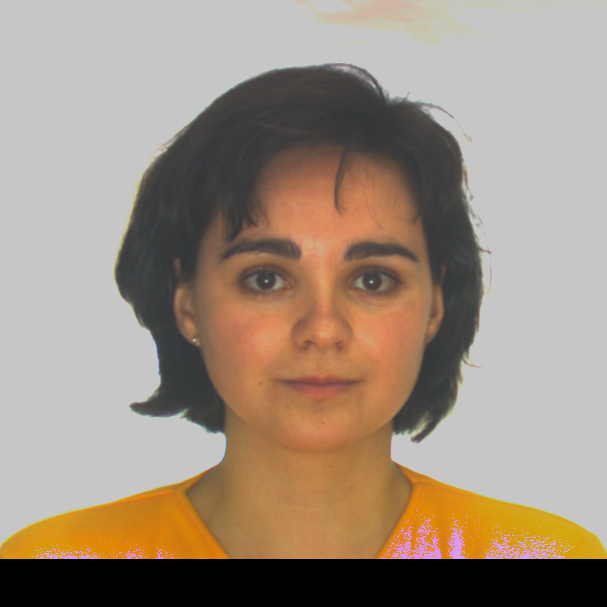
\includegraphics[width=0.23\linewidth]{images/washed_out/AR_w-054-1_C40.png}}
\caption{Example of preprocessed non-compliant images from the \washedout requirement. Source: own elaboration.}
\label{fig:washedout}
\end{figure}

\begin{figure}[t]
\centering
\subfigure[original image]{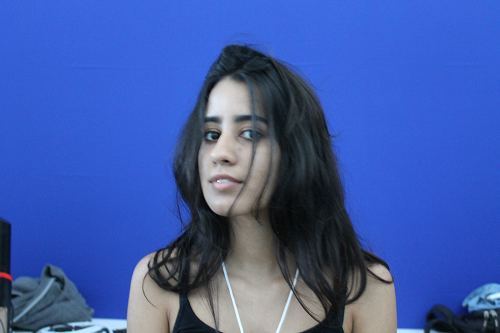
\includegraphics[height=1.5in]{images/varied_background/visio_icao_expotec_56.png}}
\hspace{0.5in}
\subfigure[preprocessed image]{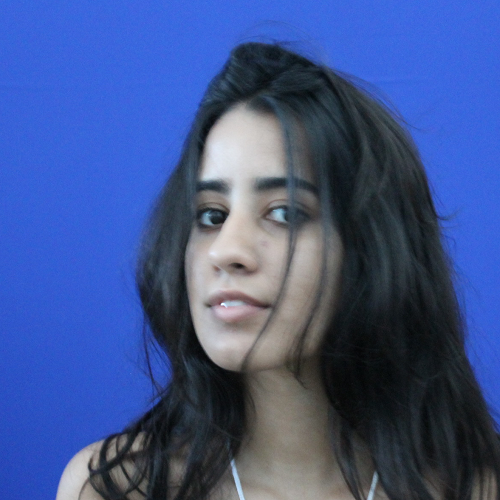
\includegraphics[height=1.5in]{images/varied_background/visio_icao_expotec_56_preprocessed.png}}
\caption{Example of a non-compliant image from the \variedbackground requirement before and after the preprocessing step. Source: own elaboration.}
\label{fig:variedbgd}
\end{figure}

\begin{figure}[t]
\centering
\subfigure[before resize (1715x1715)]{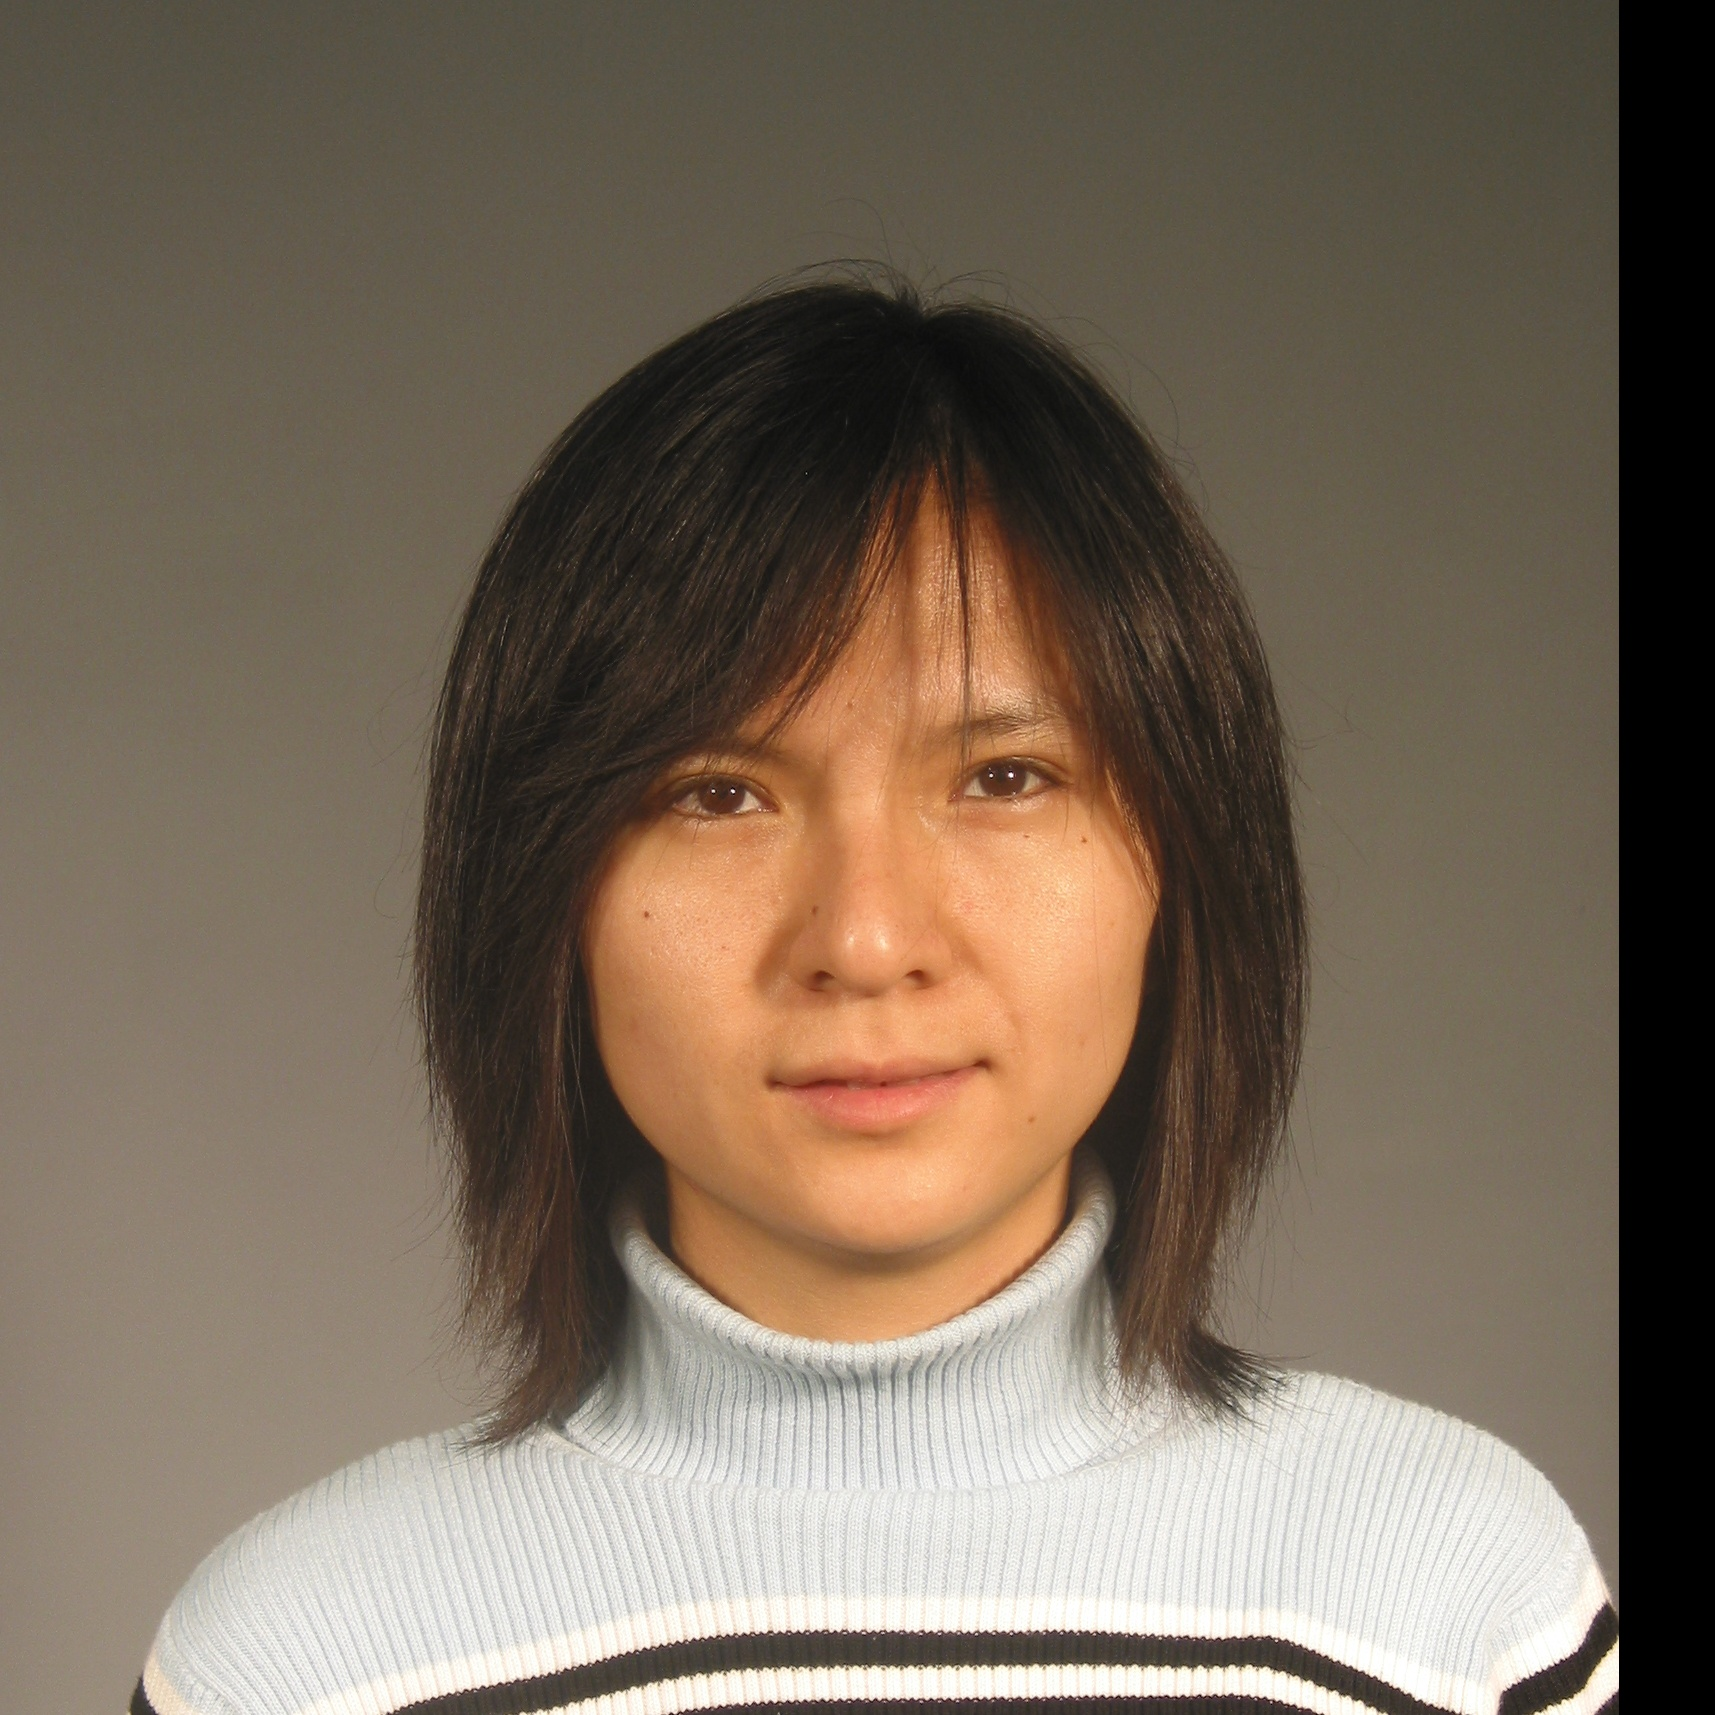
\includegraphics[height=2in]{images/hair_across_eyes/Fall2003_04853d17_preprocessed.jpg}}
\hspace{0.5in}
\subfigure[after resize (160x160)]{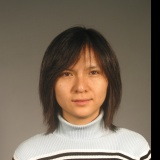
\includegraphics[height=2in]{images/hair_across_eyes/Fall2003_04853d17_resized.jpg}}
\caption{Example of a non-compliant image from the \hairacrosseyes requirement before and after the resizing operation performed by the preprocessing step. Source: own elaboration.}
\label{fig:hairacrosseyes}
\end{figure}

The \autoref{fig:eer_unbalancing} shows the \acs{eer} in both FICV datasets (as in \autoref{tab:icaonet-ficv}), but ordering the requirements by the proportion of non-compliant images in the ad-hoc dataset. Through the analysis of this graph, we can make some conclusions. First, as pointed before, the performance on both datasets is similar to each other. It reinforces the premise of FICV that the \ficvtest is a representative set of the \ficvofficial dataset (see section \ref{sec:fvcongoing}). Secondly, there is a moderate correlation between the EER and the degree of unbalancing in our dataset. According to Pearson's correlation, these coefficients are -0.47 and -0.45 for the \ficvtest and \ficvofficial datasets, respectively. In other words, if the proportion of non-compliant images increases, the \acs{eer} tends to decrease. However, it is important to notice that the fifth most unbalanced requirement (\veiloverface), with only 364 non-compliant images (or 6.31\%), is the one that achieved 0.0\% of \acs{eer} in both datasets. Also, these correlations become very weak and positives ($< +0.1$) when computed starting from the seventh most unbalanced requirement (\toodarklight, with 456 non-compliant images or 7.91\%).

\begin{figure}[ht]
\centering
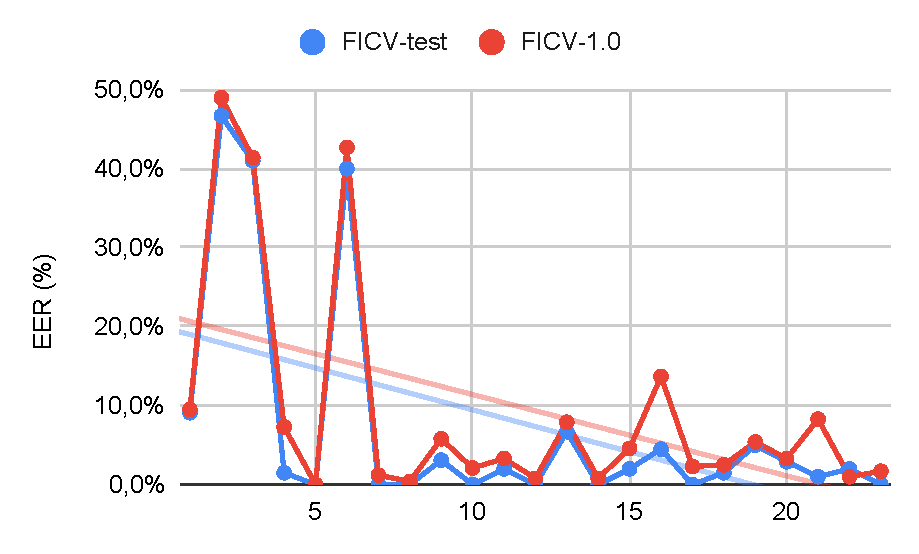
\includegraphics[width=0.8\linewidth]{images/graphs/eer_unbalancing.pdf}
\caption{EER by the proportion of non-compliant images for each requirement in ascending order. Source: own elaboration.}
\label{fig:eer_unbalancing}
\end{figure}

Regarding the eye location accuracy, the results in \acs{ficv} can be seen in \autoref{tab:eyes_ficv}. In both datasets of the competition, the results were close to the observed locally during training ($d_{eye} \in [0;0.1[ = 46.18\%$, see Section \ref{sec:eye_location_acc}). Even though $d_{eye} \in [0;0.1[$ is not as high as expected, we can notice that $d_{eye} \leq 0.2$ of \methodname is higher than $90\%$ in both official datasets. Hence, if we can improve the landmark detection of our method, acceptable levels of eye locations accuracy can be accomplished. Despite of it, significant results of tokenizable were achieved already.

% Please add the following required packages to your document preamble:
% \usepackage{booktabs}
% \usepackage{graphicx}
\begin{table}[tb]
\centering
\caption{Results of eye localization accuracy for \methodname in the official datasets of FICV competition.}
\label{tab:eyes_ficv}
\resizebox{\textwidth}{!}{%
\begin{tabular}{@{}rrrrrrr@{}}
\toprule
\textbf{} &
  \textbf{$d_{eye} \in [0;0.1[$} &
  \textbf{$d_{eye} \in [0.1;0.2[$} &
  \textbf{$d_{eye} \in [0.2;0.3[$} &
  \textbf{$d_{eye} \geq 0.3$} &
  \textbf{Rejected} &
  \textbf{Tokenizable} \\ \midrule
\ficvtest &
  43.59\% &
  46.80\% &
  4.80\% &
  4.80\% &
  0.00\% &
  88.97\% \\
\ficvofficial &
  42.68\% &
  48.24\% &
  5.46\% &
  3.62\% &
  0.00\% &
  89.19\% \\ \bottomrule
\end{tabular}%
}
\end{table}

\subsubsection{Analysis of the Worst Requirements}

% Trazer análise dos piores resultados para cá (linha 35: Three requirements had an \acs{eer} greater than 40\%) 
% e mencionar as tentativas de melhoria
% colocar um asterisco no resultado de Pixelation da tabela 6 com uma nota de rodapé, indicando que aquele resultado foi melhorado e citando esse seção

\subsection{Comparison Against Other Methods}

We start by comparing the results of \methodname with well-known architectures fine-tuned for \icao requirements. Because of the \acs{ficv} constraint for submission files (up to 50MB, see Section \ref{sec:fvcongoing}), only three architectures could be evaluated in the competition: MobileNet v1/v2 and NasNetMobile. As can be seen in \autoref{tab:comp_finetune}, \methodname outperforms the other architectures in almost all requirements (18 out of 23). There is a draw for \veiloverface, in which MobileNet v1/v2 and our method achieved 0\% of EER. Also, MobileNet v1 was able to achieve the best results in 3 other requirements (\pixelation, \hatcap, and \otherfacesortoys), while NasNet had the worst results within all methods compared. In addition, \methodname obtained the lowest results in terms of mean/median \acs{eer}, running time, and memory consumption. Finally, by these results, we can conclude the \acl{mtl} approach employed by the method proposed can perform better in practice than some networks fine-tuned for \icao.

A detailed analysis of the results shown in \autoref{tab:comp_finetune} can expose some interesting patterns. First, we can cite the eyes-related requirements. For \lookingaway, \eyesclosed, \redeyes, \darktintedlenses, \flashlenses, \framestooheavy, and \framecoveringeyes, our method achieved considerable improvements in terms of \acs{eer} (more than 50\% lower). In fact, the only requirement related to eyes that our method accomplished similar results with the other architectures was \hairacrosseyes. As mentioned before (see Section \ref{sec:ficv_results}), this results was probably influenced by our preprocessing step. We can also observe noticeable improvements for light-related requirements as \toodarklight, \shadowsbehindhead and \shadowsacrossface. Finally, when considering the highest unbalanced requirements, the proposed method also accomplished high \acs{eer} values for \inkmarked and \otherfacesortoys, but substantially lower values for \washedout and \framestooheavy.

% Please add the following required packages to your document preamble:
% \usepackage{graphicx}
\begin{table}[tb]
\centering
\caption{Comparison of the \methodname against fine-tuned versions of well-known architectures in \ficvofficial dataset.}
\label{tab:comp_finetune}
\resizebox{\textwidth}{!}{%
\begin{tabular}{clrrrr}
\hline
\textbf{Req. \#} &
  \textbf{Requirement description} &
  \multicolumn{1}{c}{\textbf{\begin{tabular}[c]{@{}c@{}}MobileNet\\ v1\end{tabular}}} &
  \multicolumn{1}{c}{\textbf{\begin{tabular}[c]{@{}c@{}}MobileNet\\ v2\end{tabular}}} &
  \multicolumn{1}{c}{\textbf{NasNet}} &
  \multicolumn{1}{c}{\textbf{\methodname}} \\ \hline
\textbf{08} & Blurred                           & 2.1           & \textbf{1.9} & 4.8   & 2.1           \\
\textbf{09} & Looking away                      & 17.3          & 26.3         & 23.1  & \textbf{5.4}  \\
\textbf{10} & Ink marked/creased                & 50            & 49.3         & 51.0  & \textbf{49.0} \\
\textbf{11} & Unnatural skin tone               & 18.5          & 19.0         & 24.0  & \textbf{1.7}  \\
\textbf{12} & Too dark/light                    & 7.7           & 7.1          & 6.7   & \textbf{1.2}  \\
\textbf{13} & Washed out                        & 15.6          & 12.3         & 23.7  & \textbf{7.3}  \\
\textbf{14} & Pixelation                        & \textbf{24.2} & 30.7         & 27.3  & 29.0          \\
\textbf{15} & Hair across eyes                  & 15.2          & 14.8         & 21.5  & \textbf{13.7} \\
\textbf{16} & Eyes closed                       & 9.2           & 14.8         & 24.2  & \textbf{0.8}  \\
\textbf{17} & Varied Background                 & 9.4           & 10.4         & 13.7  & \textbf{8.3}  \\
\textbf{18} & Roll/pitch/yaw                    & 10.6          & 9.6          & 24.5  & \textbf{4.6}  \\
\textbf{19} & Flash reflection on skin          & 8.3           & 6.7          & 12.9  & \textbf{1.0}  \\
\textbf{20} & Red eyes                          & 28.7          & 21.5         & 14.9  & \textbf{7.9}  \\
\textbf{21} & Shadows behind head               & 13.3          & 11.4         & 15.8  & \textbf{3.3}  \\
\textbf{22} & Shadows across face               & 12.1          & 12.1         & 12.7  & \textbf{3.3}  \\
\textbf{23} & Dark tinted lenses                & 1.0           & 1.5          & 1.2   & \textbf{0.4}  \\
\textbf{24} & Flash reflection on lenses        & 1.7           & 2.5          & 3.3   & \textbf{0.8}  \\
\textbf{25} & Frames too heavy                  & 50.0          & 45.3         & 35.1  & \textbf{9.5}  \\
\textbf{26} & Frame covering eyes               & 19.6          & 19.6         & 26.2  & \textbf{2.5}  \\
\textbf{27} & Hat/cap                           & \textbf{0.6}  & 1.9          & 1.0   & 5.8           \\
\textbf{28} & Veil over face                    & \textbf{0.0}  & \textbf{0.0} & 0.2   & \textbf{0.0}  \\
\textbf{29} & Mouth open                        & 11.7          & 11.7         & 17.7  & \textbf{2.3}  \\
\textbf{30} & Presence of other faces           & \textbf{36.7} & 45.5         & 48.4  & 41.4          \\ \hline
            & \multicolumn{1}{r}{mean (\%)}      & 15.8          & 16.4         & 18.9  & \textbf{8.8}  \\
            & \multicolumn{1}{r}{median (\%)}    & 12.1          & 12.1         & 17.7  & \textbf{3.3}  \\
            & \multicolumn{1}{r}{avg. time (s)} & 2.9           & 3.1          & 4.2   & \textbf{1.8}  \\
            & \multicolumn{1}{r}{max. time(s)}  & 3.4           & 4.2          & 5.2   & \textbf{3.3}  \\
            & \multicolumn{1}{r}{memory (MB)}   & 332.2         & 322.5        & 377.5 & \textbf{313} 
\end{tabular}%
}
\end{table}

Table \ref{tab:best-results} summarizes the best results by requirement among all the methods shown in Table \ref{tab:comp}. Also, it includes the results of \methodname for easy comparison. All methods were evaluated using the FICV competition benchmark tool and the official dataset (\ficvofficial). As can be seen, the proposed method has the best results in 9 out of 23 requirements of the \icao standard. Thus, the proposed method has the highest amount of best results in terms of requirements. We can also notice that \methodname has low rejection rates, with only four requirements rejecting at most 0.4\% of the evaluated images. Such rejections represent the false negatives from the face detector used to preprocess input images.

% Please add the following required packages to your document preamble:
% \usepackage[table,xcdraw]{xcolor}
% If you use beamer only pass "xcolor=table" option, i.e. \documentclass[xcolor=table]{beamer}
\begin{table}[!tb]
\centering
\caption{Comparison of the \methodname against the best results reported in the literature and by private SDK tools (see Table \ref{tab:comp}). All methods were evaluated by the benchmark tool of FICV using the \ficvofficial dataset.}
\label{tab:best-results}
\begin{tabular}{ccrrrr}
\hline
 & \multicolumn{3}{c}{\textbf{\begin{tabular}[c]{@{}c@{}}Best of Literature/\\ Commercial SDK\end{tabular}}} & \multicolumn{2}{c}{\textbf{ICAONet}} \\ \hline
\textbf{Req. \#} & Method & \multicolumn{1}{c}{EER} & \multicolumn{1}{c|}{{\color[HTML]{9B9B9B} Rej.}} & \multicolumn{1}{c}{EER} & \multicolumn{1}{c}{{\color[HTML]{9B9B9B} Rej.}} \\ \cline{2-6} 
\textbf{08} & BioPass Face & 1.60 & {\color[HTML]{9B9B9B} 3.30} & 2.10 & {\color[HTML]{9B9B9B} 0.60} \\
\textbf{09} & HMAX & 10.00 & {\color[HTML]{9B9B9B} 0.16} & \textbf{5.40} & {\color[HTML]{9B9B9B} 0.00} \\
\textbf{10} & BioLab & 3.40 & {\color[HTML]{9B9B9B} 1.20} & 49.00 & {\color[HTML]{9B9B9B} 0.00} \\
\textbf{11} & BioPass Face & 1.90 & {\color[HTML]{9B9B9B} 0.00} & \textbf{1.70} & {\color[HTML]{9B9B9B} 0.00} \\
\textbf{12} & id3 & 2.90 & {\color[HTML]{9B9B9B} 0.00} & \textbf{1.20} & {\color[HTML]{9B9B9B} 0.00} \\
\textbf{13} & BioPass Face & 0.00 & {\color[HTML]{9B9B9B} 0.00} & 7.30 & {\color[HTML]{9B9B9B} 0.00} \\
\textbf{14} & SDK 2 & 0.00 & {\color[HTML]{9B9B9B} 0.00} & 29.00 & {\color[HTML]{9B9B9B} 0.00} \\
\textbf{15} & Parente et al. & {\color[HTML]{333333} 11.90} & {\color[HTML]{9B9B9B} 3.40} & 13.70 & {\color[HTML]{9B9B9B} 0.40} \\
\textbf{16} & id3 & 0.20 & {\color[HTML]{9B9B9B} 1.00} & 0.80 & {\color[HTML]{9B9B9B} 0.00} \\
\textbf{17} & BioTest & 3.70 & {\color[HTML]{9B9B9B} 7.90} & 8.40 & {\color[HTML]{9B9B9B} 1.30} \\
\textbf{18} & id3 & 9.10 & {\color[HTML]{9B9B9B} 6.90} & \textbf{4.60} & {\color[HTML]{9B9B9B} 0.20} \\
\textbf{19} & BioLab & 0.60 & {\color[HTML]{9B9B9B} 0.00} & 1.00 & {\color[HTML]{9B9B9B} 0.00} \\
\textbf{20} & id3 & 1.00 & {\color[HTML]{9B9B9B} 2.00} & 8.20 & {\color[HTML]{9B9B9B} 1.50} \\
\textbf{21} & BioLab & 2.30 & {\color[HTML]{9B9B9B} 0.20} & 3.30 & {\color[HTML]{9B9B9B} 0.00} \\
\textbf{22} & Andrezza et al. & 7.70 & {\color[HTML]{9B9B9B} 2.50} & \textbf{3.30} & {\color[HTML]{9B9B9B} 0.20} \\
\textbf{23} & BioPass Face & 1.80 & {\color[HTML]{9B9B9B} 1.20} & \textbf{0.40} & {\color[HTML]{9B9B9B} 0.00} \\
\textbf{24} & BioLab & 2.10 & {\color[HTML]{9B9B9B} 0.00} & \textbf{0.80} & {\color[HTML]{9B9B9B} 0.00} \\
\textbf{25} & HMAX & 0.00 & {\color[HTML]{9B9B9B} 0.00} & 9.50 & {\color[HTML]{9B9B9B} 0.00} \\
\textbf{26} & HMAX & 0.00 & {\color[HTML]{9B9B9B} 0.10} & 2.30 & {\color[HTML]{9B9B9B} 0.60} \\
\textbf{27} & id3 & 6.80 & {\color[HTML]{9B9B9B} 0.80} & \textbf{5.70} & {\color[HTML]{9B9B9B} 0.20} \\
\textbf{28} & Parente et al. & 1.20 & {\color[HTML]{9B9B9B} 0.50} & \textbf{0.00} & {\color[HTML]{9B9B9B} 0.00} \\
\textbf{29} & id3 & 0.60 & {\color[HTML]{9B9B9B} 0.40} & 2.30 & {\color[HTML]{9B9B9B} 0.00} \\
\textbf{30} & BioPass Face & 1.20 & {\color[HTML]{9B9B9B} 2.70} & 41.40 & {\color[HTML]{9B9B9B} 0.00} \\ \hline
\multicolumn{4}{r}{\textbf{mean (\%)}} & 8.80 & 0.22 \\
\multicolumn{4}{r}{\textbf{median (\%)}} & 3.30 & 0.00 \\
\multicolumn{4}{r}{\textbf{avg. time (s)}} & \multicolumn{2}{c}{2.7} \\
\multicolumn{4}{r}{\textbf{max. time (s)}} & \multicolumn{2}{c}{3.4} \\
\multicolumn{4}{r}{\textbf{memory (MB)}} & \multicolumn{2}{c}{306.1}
\end{tabular}
\end{table}

There are four methods with public results published in the \fvcongoing: BioPass Face \citep{fvcVsoft}, BioTest \citep{fvcBioTest}, id3 \citep{fvcICAOCompliance}, and ICAOSDK \citep{fvcSeamfix}. In comparison to them, we have the best results in 11 out of all 23 requirements. Therefore, the \methodname is also the method with the highest amount of best results in terms of requirements in the FICV competition. Additionally, the proposed method has the second-best Median EER (3.3\%).

In terms of performance, the \methodname takes on average 1.8 seconds per image according to the official benchmark results on the FICV competition of the \fvcongoing website. In comparison with methods that evaluate all requirements, the proposed method is the fastest. However, according to our benchmarks, almost 90\% of the \methodname running time is dominated by the face detector (1.6s on average), which is a preprocessing step. On the other hand, the architecture of the proposed network takes only 0.15s of this total time. Furthermore, since the FICV competition runs the benchmarks in CPU-only computers, our network could be even faster by using a GPU. In the future, we intend to change our face detector to a faster alternative so that our total time in CPU will be reduced even more.

To improve these results, two distinct approaches can be followed. First, our dataset quality can be improved by increasing (i) the number of images and (ii) the variability of patterns of some requirements (like hat/cap). Thereby, the network can learn more effective descriptors and decrease our EER in these requirements. Secondly, we may change the network or try other loss functions. For instance, we can test loss functions designed for multi-label classification problems, like the Contrastive Loss \citep{khosla2020supervised}.

With respect to eye location accuracy, \autoref{tab:comp_eyes} compares the \methodname with the other methods published in the \acs{ficv} competition. Despite \methodname has the worst performance for $d_{eye} \in [0;0.1[$ ($42.68\%$), as discussed before, our $d_{eye} \leq 0.2$ is greater than 90\%. Thus, if we improve our landmark prediction, we can achieve performance results comparable to \biopass and id3 methods. Moreover, it is important to highlight that \methodname is the only method that does not reject images. Finally, the landmarks detected by our method are already able to allow the tokenization of almost 90\% of the input images, being better than \biotest algorithm.

We believe the most effective way to improve our landmark predictions is by improving our dataset. First, the amount of samples must be increased to follow other landmark datasets with hundreds of thousands images. Furthermore, the variation of landmarks is an important factor as well. It includes, for example, more face positions with a higher range of head rotations in all axis (which can not be achieved by classic image augmentation techniques). Lastly, we could also try other custom loss functions specially designed for landmark localization.

% Please add the following required packages to your document preamble:
% \usepackage{booktabs}
% \usepackage{graphicx}
\begin{table}[tb]
\centering
\caption{Results of eye localization accuracy for the methods with published results in the FICV competition.}
\label{tab:comp_eyes}
\resizebox{\textwidth}{!}{%
\begin{tabular}{@{}rrrrrrr@{}}
\toprule
\textbf{} &
  \textbf{$d_{eye} \in [0;0.1[$} &
  \textbf{$d_{eye} \in [0.1;0.2[$} &
  \textbf{$d_{eye} \in [0.2;0.3[$} &
  \textbf{$d_{eye} \geq 0.3$} &
  \textbf{Rejected} &
  \textbf{Tokenizable} \\ \midrule
\biopass    & 94.46\% &  2.00\% & 1.49\% & 0.65\% & 1.41\%  & 92.86\% \\
id3         & 95.46\% &  2.11\% & 0.73\% & 0.38\% & 1.32\%  & 95.03\% \\
\biotest    & 77.08\% &  5.08\% & 0.89\% & 2.73\% & 14.22\% & 78.22\% \\
\methodname & 42.68\% & 48.24\% & 5.38\% & 3.41\% &  0.30\% & 89.05\% \\ \bottomrule
\end{tabular}%
}
\end{table}

\subsection{Network Visualization} \label{sec:netviz}

In addition to the performance results already presented, we decided to apply different techniques to understand the network outputs. First, we analyzed the embeddings learned by the network using algorithms for dimensionality reduction. Secondly, we applied network visualization techniques to understand which image regions are the most relevant to each requirement. More details can be found in the following paragraphs.

A visualization of the embeddings learned by \methodname is shown in the 3D plots of Figure \ref{fig:embviz}. The embedding dimension was reduced to 3 dimensions and visualized via the PCA and t-SNE methods using TensorBoard\footnote{https://www.tensorflow.org/tensorboard}. Each point in the plot is represented by a face image from the dataset. Although the figure shows only three dimensions, it is possible to observe that some dimensions are related to particular ICAO requirements. For example, in the figure related to PCA, we can observe that images with \variedbackground, \unnaturalskintone, and \veiloverface are closer to each other in a certain degree. On the other hand, in t-SNE, we can notice that the clusters related to such requirements are more well defined, especially for \variedbackground and \veiloverface requirements. Moreover, in both figures, we can see the intersection between some regions. For instance, images with unnatural skin tone and veil over face tend to belong to both clusters. Such information is relevant to the multi-task classification branch of the \methodname architecture. 

\begin{figure}[ht]
\centering
\subfigure[PCA]{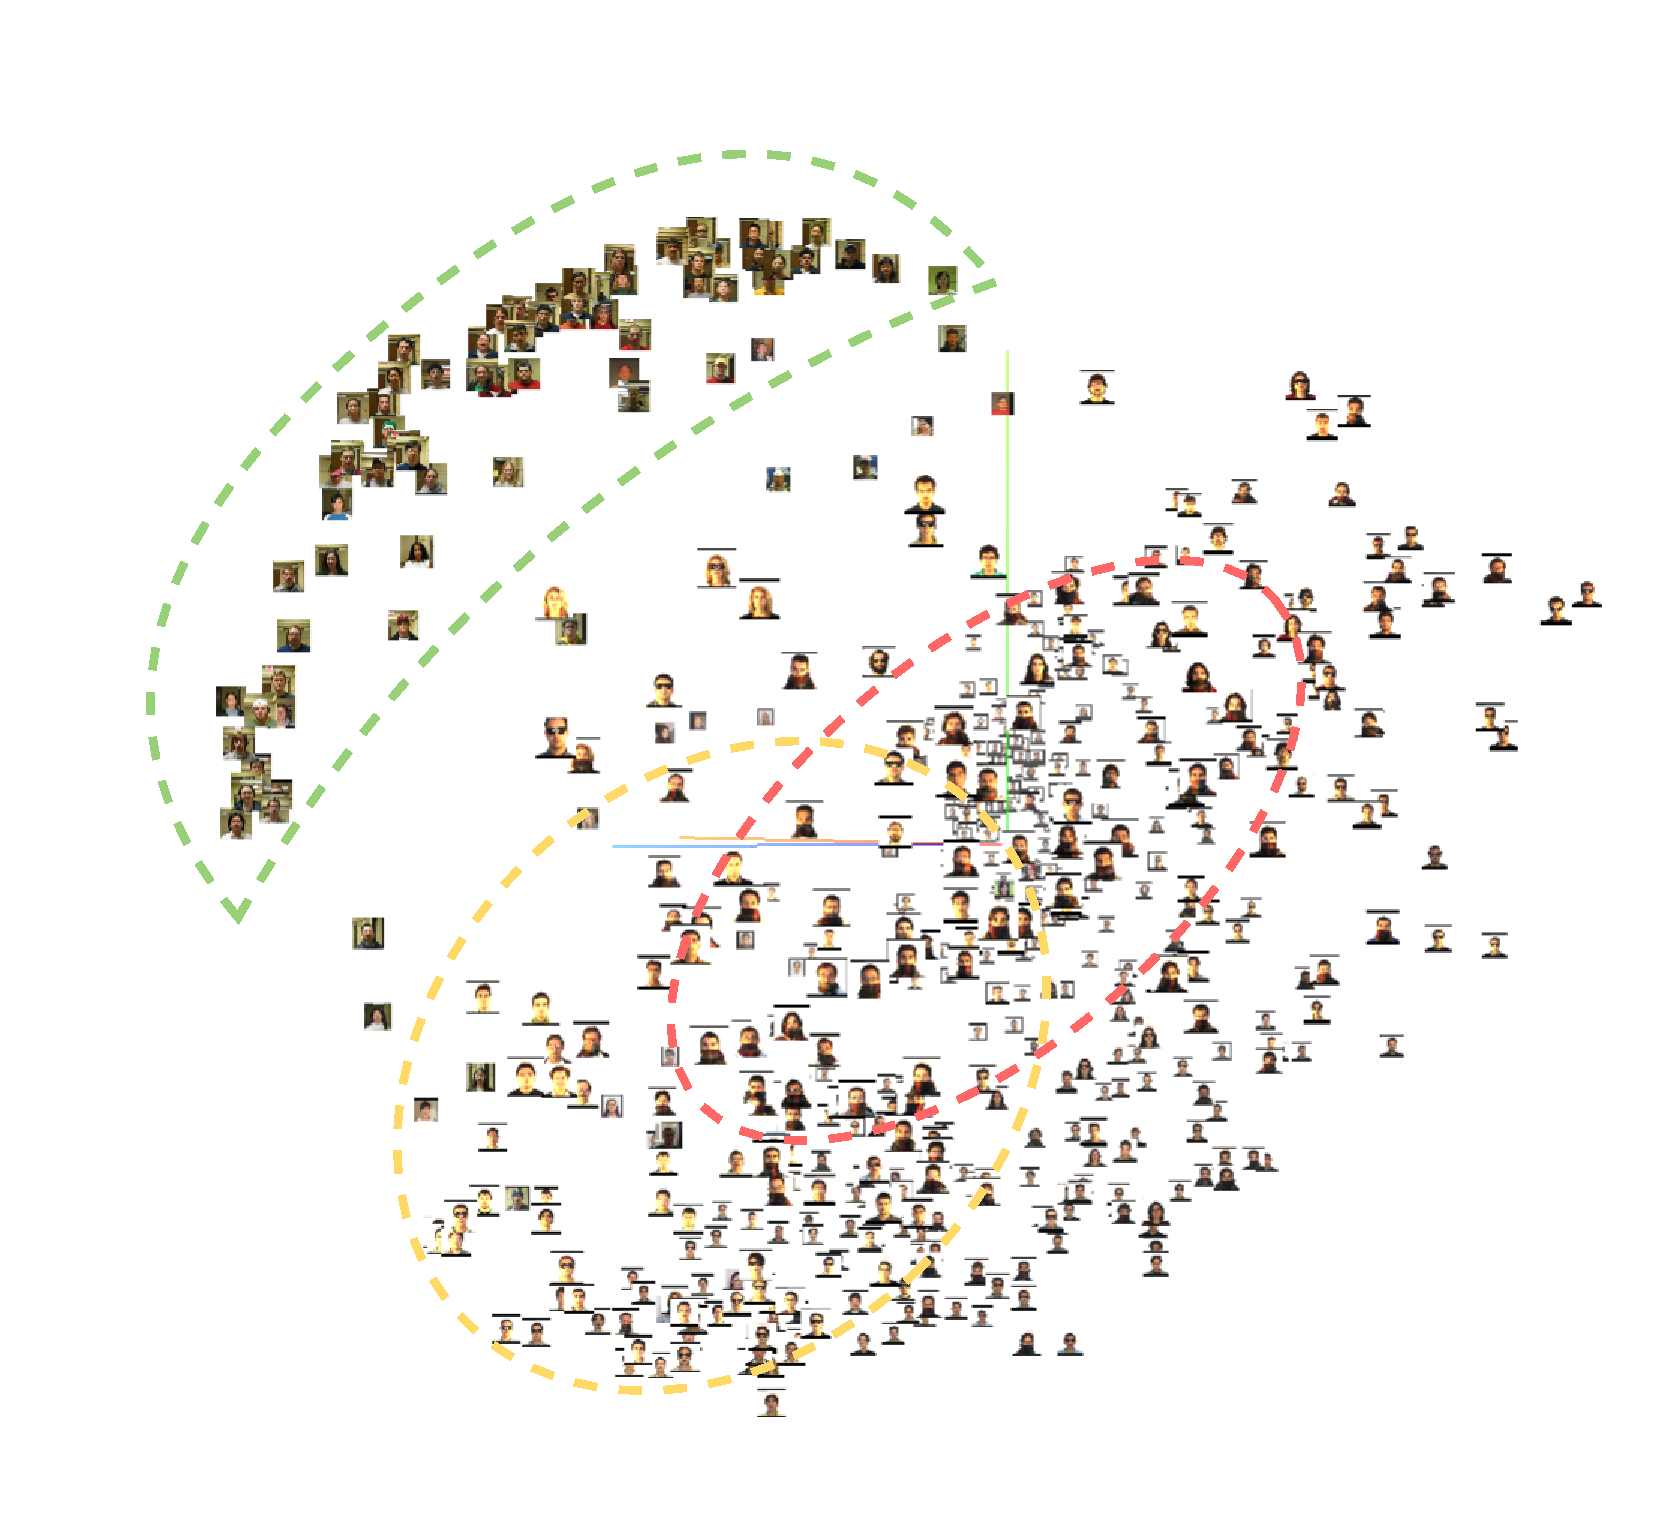
\includegraphics[width=0.75\linewidth]{images/pca.pdf}}
\subfigure[t-SNE]{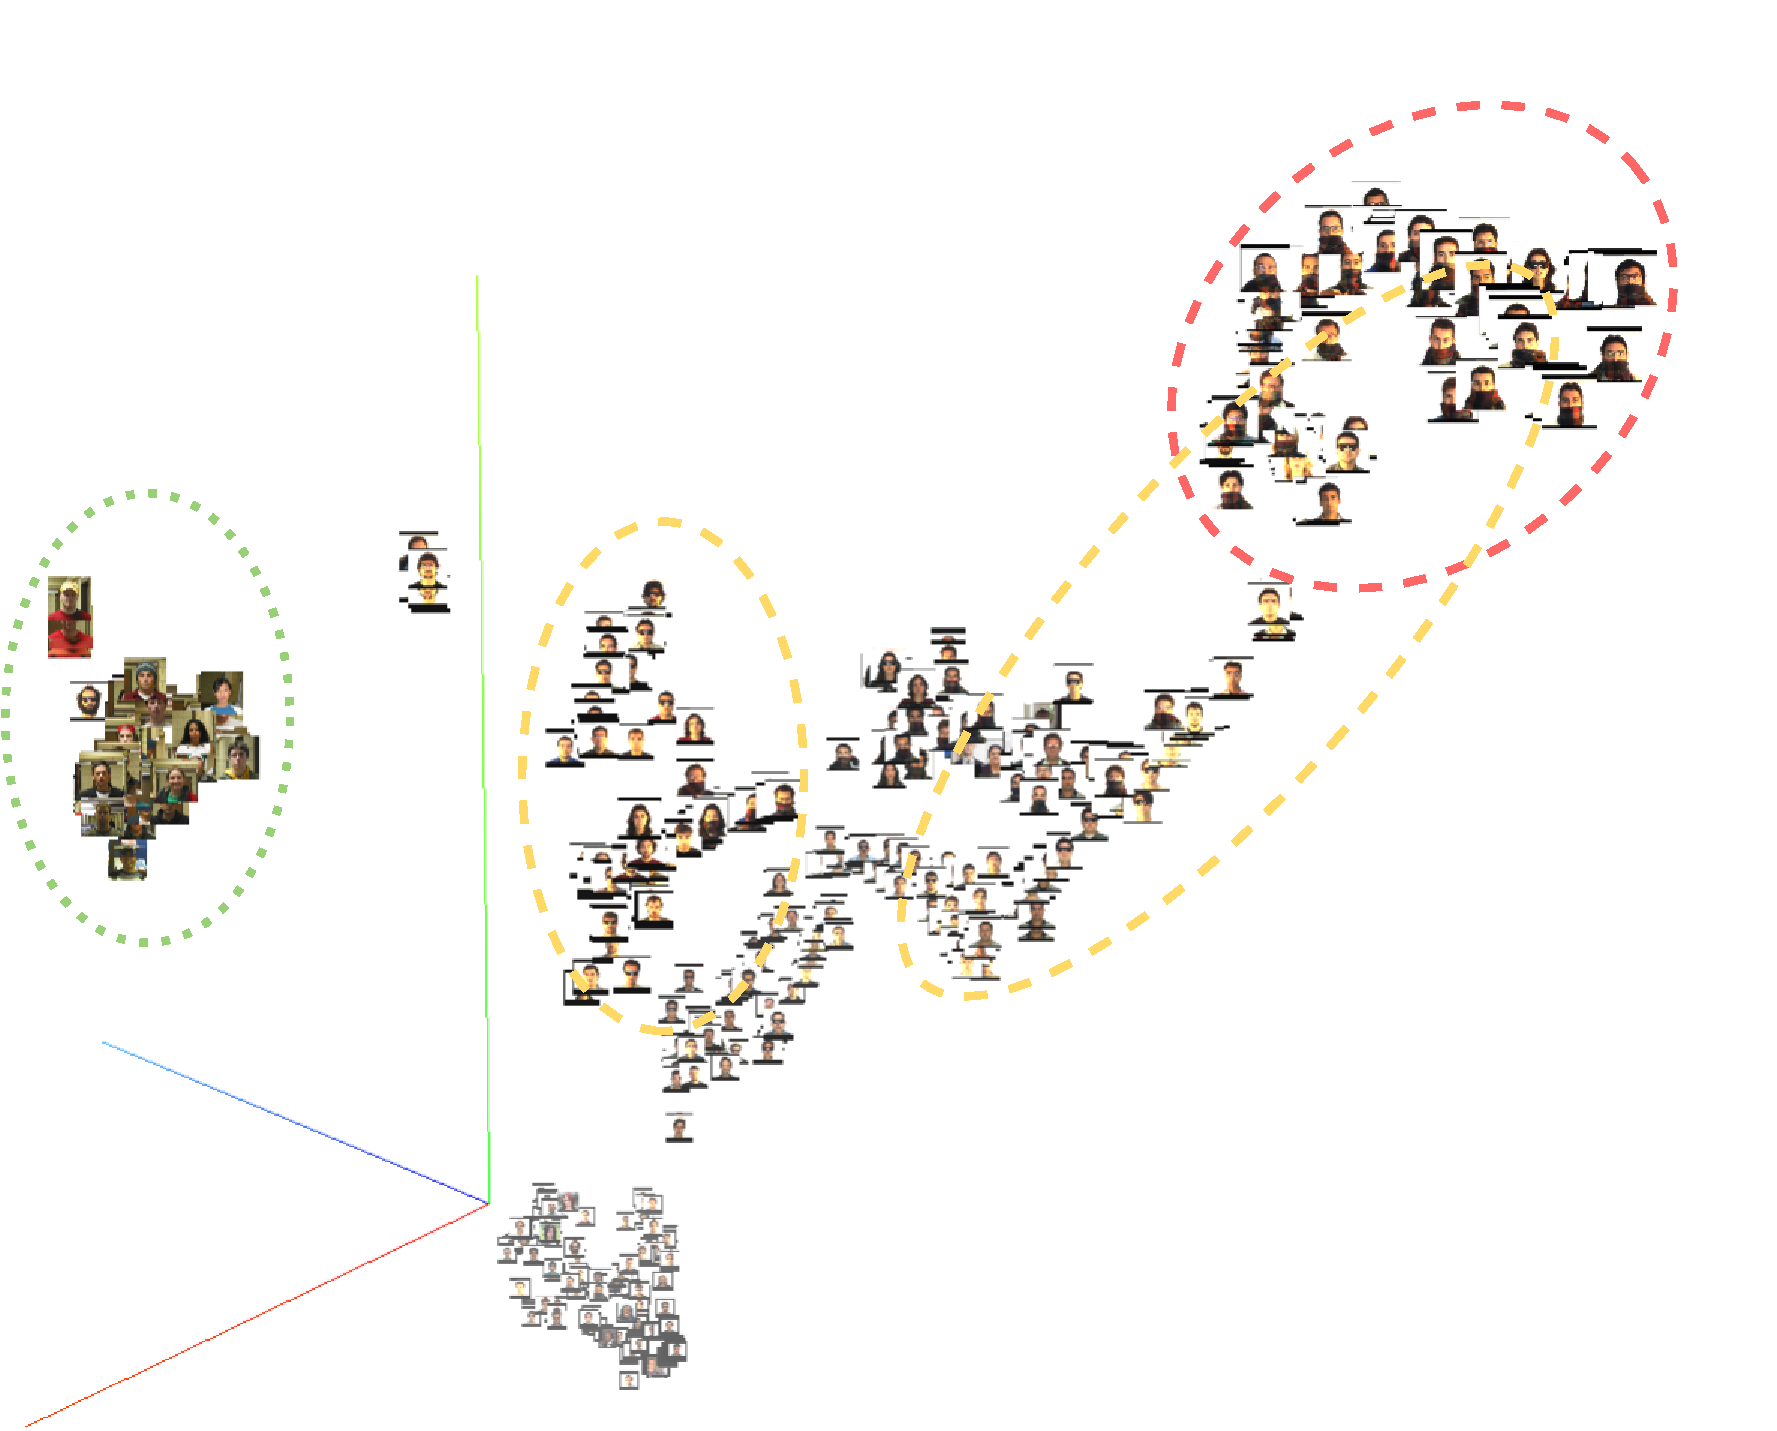
\includegraphics[width=0.75\linewidth]{images/tsne.pdf}}    
\caption{Visualization of the embeddings learned by \methodname. Original embeddings dimensions were reduced to 3D using (a) PCA and (b) t-SNE. In both visualizations, we highlight the regions of \variedbackground (green), \unnaturalskintone (yellow), and \veiloverface (red) requirements. Source: own elaboration.}
\label{fig:embviz}
\end{figure}

Figure \ref{fig:shap} contains a visual representation of input images with local region contributions associated with each pose and photograph requirements. The SHAP method was used to create that visualization. The figure provides evidence that the network learned useful representations for most of the requirements. In the fully compliant images (first three rows), the classification output is usually increased by the image regions related to that requirement. For example, in the eye-region dependent requirements (09, 15, 16, 20, 23, 24, and 26), the output is mainly influenced by regions closer to the eyes. Similar behaviors can be observed in requirements related to the mouth (28 and 29), skin (11, 19, 22), and the image aspect (08, 12, 13). 

However, we can notice the network was not able to learn relevant patterns in some requirements like \inkmarked, \pixelation, \framestooheavy, \hatcap, and \otherfacesortoys. For requirements 10, 25, and 30, we believe the low amount of non-compliant images was the most crucial factor in contributing to the worst results of the proposed architecture, found in Table \ref{tab:req-dist}. In the case of \pixelation, a possible cause for the high EER (42.7\%) could be the image resizing step applied in the input images. Finally, the random patterns in \hatcap may show that the variability of head props in our dataset must be insufficient to distinguish them from other patterns. 

\begin{landscape}
\begin{figure*}[ht]
\centering
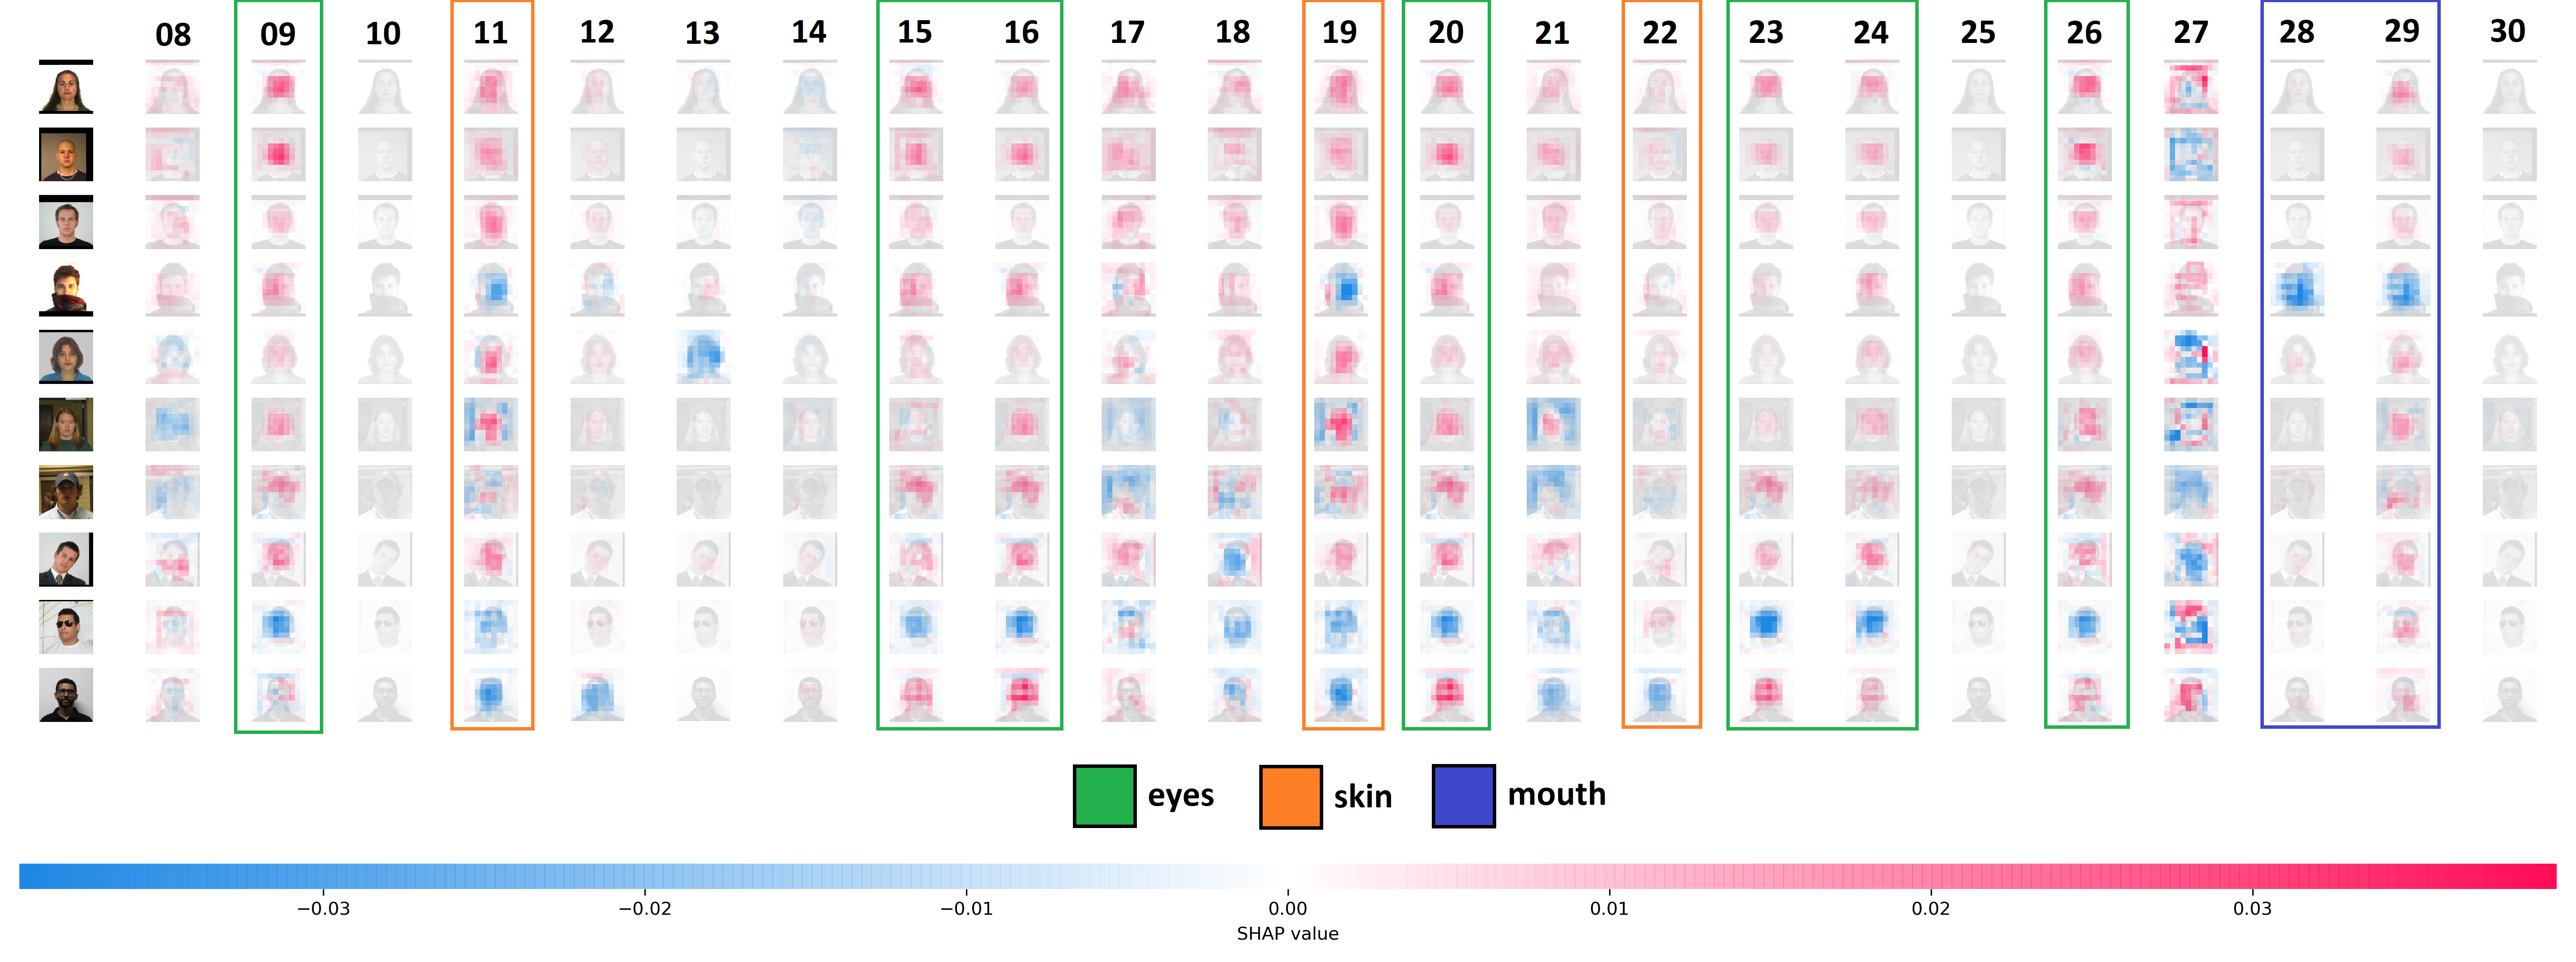
\includegraphics[width=\linewidth]{images/shap.png}
\caption{Visual explanation of \methodname's output using SHAP. The rows represent input images, and the columns denote the requirements from the \icao standard. The first three images are fully compliant, while the remaining images have at least one non-compliant requirement. According to the SHAP values, each pixel contributes negatively (blue), positively (red), or has a low contribution (white) to the network's output. Some requirements related to eyes, skin, and mouth are highlighted for convenience. Source: own elaboration.}
\label{fig:shap}
\end{figure*}
\end{landscape}

\section{Concluding Remarks}

This thesis presented a deep learning-based method developed to evaluate photographic requirements and eye location accuracy of \icao standard, called \methodname. Our method extends undercomplete Convolutional Autoencoders with supervised branches that performs multi-label classification and landmark regression in a collaborative fashion with unsupervised learning. The architecture has three main components: (i) an encoder to encode the input image into a proper 256-D representation shared by (ii) an unsupervised branch to reconstruct the input image; and (iii) supervised branches to assess the requirements as a multi-label problem, determine the eye-center positions as a regression problem, and classify the specific \pixelation requirement as a binary classification task.

We can consider that \methodname presented valuable advances in its research field. First, compared to other encoder-focused architectures available in the literature, the proposed method does not require pre-training and is easy to scale. Secondly, \acl{mtl} was leveraged with different learning techniques (supervised and unsupervised) and tasks (regression and binary/multi-label classification). Regarding Representation Learning, the proposed architecture also employs both generative and discriminative approaches. Therefore, the method learned a functional representation built from related tasks to predict different outputs. Finally, \methodname is the first and only open-source research that evaluates all 23 photographic requirements with considerably low memory consumption and running time.

We evaluated our method using a small amount of unbalanced but stratified data. It comprises a subset of the \ficvtest dataset in conjunction with an \adhoc dataset built especially for ICAO requirements. The network was trained from scratch, and a custom loss function was used in the network optimization process. This function balances the tasks solved by the method, i.e., image reconstruction, landmark localization, and requirements assessment. Additionally, the training was monitored to preserve the model with the highest F-Beta score.

Individually, the \methodname was able to achieve significant results. In training, most of the metrics evaluated in the validation set had a score greater than 90\%. Through the analysis of these metrics, we were able to notice some patterns in the method predictions. For example, it is better to predict the positive class, but the \aclp{fp} are more troublesome than \aclp{fn}. Additionally, in the \acs{ficv} competition, the method presented a substantial performance in most requirements. Nevertheless, unacceptable performance in terms of \acs{eer} ($> 40\%$) were obtained for two requirements and the eye location accuracy was below expectations. Both results will require further work for improvement.

Compared to other methods evaluated by the \acs{ficv} benchmark, the \methodname was able to achieve state-of-art results in 9 out of 23 requirements and a global median EER of 3.3\%. Therefore, the proposed work has the highest amount of best results in a single method compared to all the works presented in the literature or private SDK tools. In terms of EER, the \methodname has the second-best median EER compared to methods that evaluate all requirements. Furthermore, the proposed method is also among the fastest methods to evaluate all requirements on the CPU, taking only 2.7s to evaluate an input image in average. However, our running time still has a spot for improvement since it is highly influenced by the face detector used for preprocessing. The architecture proposed by itself takes only 0.15s to run in the CPU.

We believe that our method was able to outperform the others for the following reasons. First, by using \acs{mtl}, the model can exploit similarities and dependencies between tasks and learn a useful set of features shared among tasks. The features learned from one task can be beneficial for related tasks, particularly when the tasks have overlapping characteristics. This is the case with the \icao standard. Furthermore, \acs{mtl} is known to handle imbalanced and limited data (like the dataset used in this thesis). Thus, we avoided the creation of a model biased to the majority class, which is also enforced by the metrics and regularization techniques applied during training.

Regarding our research question presented in Chapter \ref{sec:introduction}, we can conclude that it has been answered. In terms of efficiency, as cited previously, the proposed method is among the fastest, even without post optimization. In addition, according to the official FICV benchmark, the method was lightweight, consuming approximately 300 MB of memory. On the other hand, although \methodname was not able to achieve state-of-the-art results for all 23 requirements, we noticed that Deep \acl{mtl} can be an alternative capable of achieving low error rates. Furthermore, by applying the recommendations for future work cited below, the proposed method will likely improve the results.

As future works, we intend to concentrate efforts on three different aspects to improve the results:

\begin{itemize}
\item \textbf{Dataset}: the dataset quality can be improved by increasing (i) the number of images and (ii) the variability of patterns of some requirements (like hat/cap). Thereby, the network can learn more effective descriptors and decrease the EER in these requirements. The most unbalanced requirements may require special attention, and probably more images must be gathered. Furthermore, the dataset labels may be revised to fix possible labeling errors.

\item \textbf{Preprocessing}: as discussed in Chapter \ref{sec:results}, the preprocessing step may have been responsible for some of the errors. First, we can replace the current face detector with a faster and more reliable approach like \cite{faceboxes}. It can help to decrease the detection time (approximately 90\% of total running time) and the Rejection Rates (0.4\% max). Moreover, we must improve the input image provided to the network. For some images, the cropping and resizing steps remove or generate artifacts that can harm network learning. See Figures \ref{fig:variedbgd} and \ref{fig:hairacrosseyes} of Section \ref{sec:ficv_results} for further details. Thus, we need to find a better way to preprocess the input image as a whole without injuring the trade-off between speed and accurate results.

\item \textbf{Method}: some elements of the network can also be considered. It includes, but is not limited to, the architecture and the loss function. For example, the Capsule Neural Networks (CapsNets), proposed by \cite{sabour2017dynamic}, may help the method create hierarchical representation and capture the spatial relationships between different parts of the input image. Also, the Vision Transformers \citep{dosovitskiy2020image} can be used to capture global context information, leading to a better understanding of the image as a whole and avoiding image resizing. Recent techniques like Self-Supervised Learning \citep{doersch2017multi} may also be considered, specially for their ability to reduce annotation costs and handling noisy data. Finally, we intend to test other losses functions specially designed for the multi-label classification task. For instance, the Contrastive Loss \citep{khosla2020supervised}, designed for few-shot learning scenarios, encourages the model to learn to differentiate between similar and dissimilar pairs of data.
\end{itemize}

Finally, the present work won an award and was published in a journal, as follows:

\begin{itemize}
\item \textbf{AI Awards (2\textsuperscript{nd} place)} \citep{aiaward}: The AI Awards is a national award for Artificial Intelligence in Brazil. It is considered the highest award of the Brazilian academy for innovative postgraduate projects involving Artificial Intelligence.

\item \bibentry{icaonet}
\end{itemize}

%%%%%%%%%%%%%%%%%%%%%%%%%%%%% Referências %%%%%%%%%%%%%%%%%%%%%%%%%%%%%
\renewcommand{\refname}{\centering REFERENCES}
\small
\bibliographystyle{apalike}
\bibliography{7_referencias.bib}
%%%%%%%%%%%%%%%%%%%%%%%%%%%%%%%%%%%%%%%%%%%%%%%%%%%%%%%%%%%%%%%%%%%%%%%

\end{document}